\chapter{The Monophoton Analysis}
\label{chap:analysis}

The main event.

\section{Event Selection}
\label{sec:event_selection}

%%% need to make a second pass to change language from paper version

The integrated luminosity of the analyzed data sample is $(35.9\pm0.9)$\fbinv~\cite{CMS:2017sdi}. 
The data sample is collected with a single-photon trigger that requires at least one photon candidate with $\pt > 165\GeV$. 
The photon candidate must have $H/E < 0.1$ to discriminate against jets, where $H/E$ is the ratio of HCAL to ECAL energy deposits in the central calorimeter tower corresponding to the candidate.
The photon energy reconstructed at the HLT is less precise relative to that derived later in the offline reconstruction. 
Therefore, the thresholds in the trigger on both $H/E$ and \ETg, are less restrictive than their offline counterparts.  
The trigger efficiency is measured to be about 98\% for events passing the analysis selection with $\ETg > 175\GeV$.

From the recorded data, events are selected by requiring $\met > 170\GeV$ and at least one photon with $\ETg > 175\GeV$ in the fiducial region of the ECAL barrel ($\abs{\eta} < 1.44$) passing the selected presented in Section~\ref{sec:photons}. 

Events with a high-\pt\ photon and large \met\ are subjected to further requirements to suppress SM background processes that feature a genuine high-energy photon, but not a significant amount of \met.
One such SM process is \gj, where an apparent large \met\ is often the result of a mismeasured jet energy.
In contrast to signal processes, \met is typically smaller than \ETg\ in these events, so requiring the ratio of \ETg\ to \met to be less than 1.4 rejects this background effectively with little effect on signal efficiency. 
Events are also rejected if the minimum opening angle between \ptvecmiss\ and the directions of the four highest \pt\ jets, \minDphiMETj, is less than 0.5. 
Only jets with $\PT > 30\GeV$ and $\abs{\eta} < 5$ are considered in the \minDphiMETj\ calculation. 
In the \gj\ process, rare pathological mismeasurement of \ETg\ can also lead to large \met. 
For this reason, the candidate photon \ptvec\ and \ptvecmiss\ must be separated by more than 0.5 radians. 
Another SM process to be rejected is \wlng, for which events are vetoed if they contain an electron or a muon with $\pt > 10\GeV$ that is separated from the photon by $\dR > 0.5$.
Furthermore, using features described in Section~\ref{sec:beam_halo}, the signal region is split into two parts according to $\phi$ to constrain the beam halo normalization. 
The region defined by $\abs{\sin(\phi)} < \sin(0.5)$ is called the horizontal region, and its complement in $\phi$ is called the vertical region.

The residual contributions from the \wlng\ process, where the lepton could not be identified or was out of the detector acceptance, are modeled by fitting to observed data, as described in Section~\ref{sec:irreducible}. 
The same method is employed to model the contribution from the \zinvg\ process to the signal region. 
This method utilizes control regions where one or two leptons (electrons or muons) are identified in addition to the photon, as defined in the following.

The single-electron (single-muon) control region is defined by a requirement of exactly one electron (muon) with $\pt > 30\GeV$ and $\abs{\eta} < 2.5\,(2.4)$ in addition to a photon requirement that is identical to the one for the signal region. 
To suppress the contributions from large-\met\ processes other than \wlng, the transverse mass $\mt = \sqrt{\smash[b]{2\met\PT^{\ell}[1-\cos\Delta\phi(\ptvecmiss,\ptvefg
c^{\ell})]}}$ must be less than $160\GeV$.
Additionally, for the single-electron control region, \met\ must be greater than 50\GeV\ to limit the contribution from the \gj\ process, where a jet is misidentified as an electron. 
Finally, the recoil vector $\vec{U} = \ptvecmiss + \ptvec^{\ell}$, which serves as this region's analogue for \ptvecmiss\ in the signal region, must satisfy identical requirements to those for the \ptvecmiss\ in the signal region.

The dielectron (dimuon) control region is defined by exactly two electrons (muons) in addition to the photon, with $60 < m_{\ell\ell} < 120\GeV$, where $m_{\ell\ell}$ is the invariant mass of the dilepton system. 
The recoil vector of this region is $\vec{U} = \ptvecmiss + \sum\ptvec^{\ell}$ and must satisfy identical requirements to those for the \ptvecmiss\ in the signal region.

\section{Irreducible backgrounds}
\label{sec:irreducible}

\begin{figure}[htbp]
  \centering
    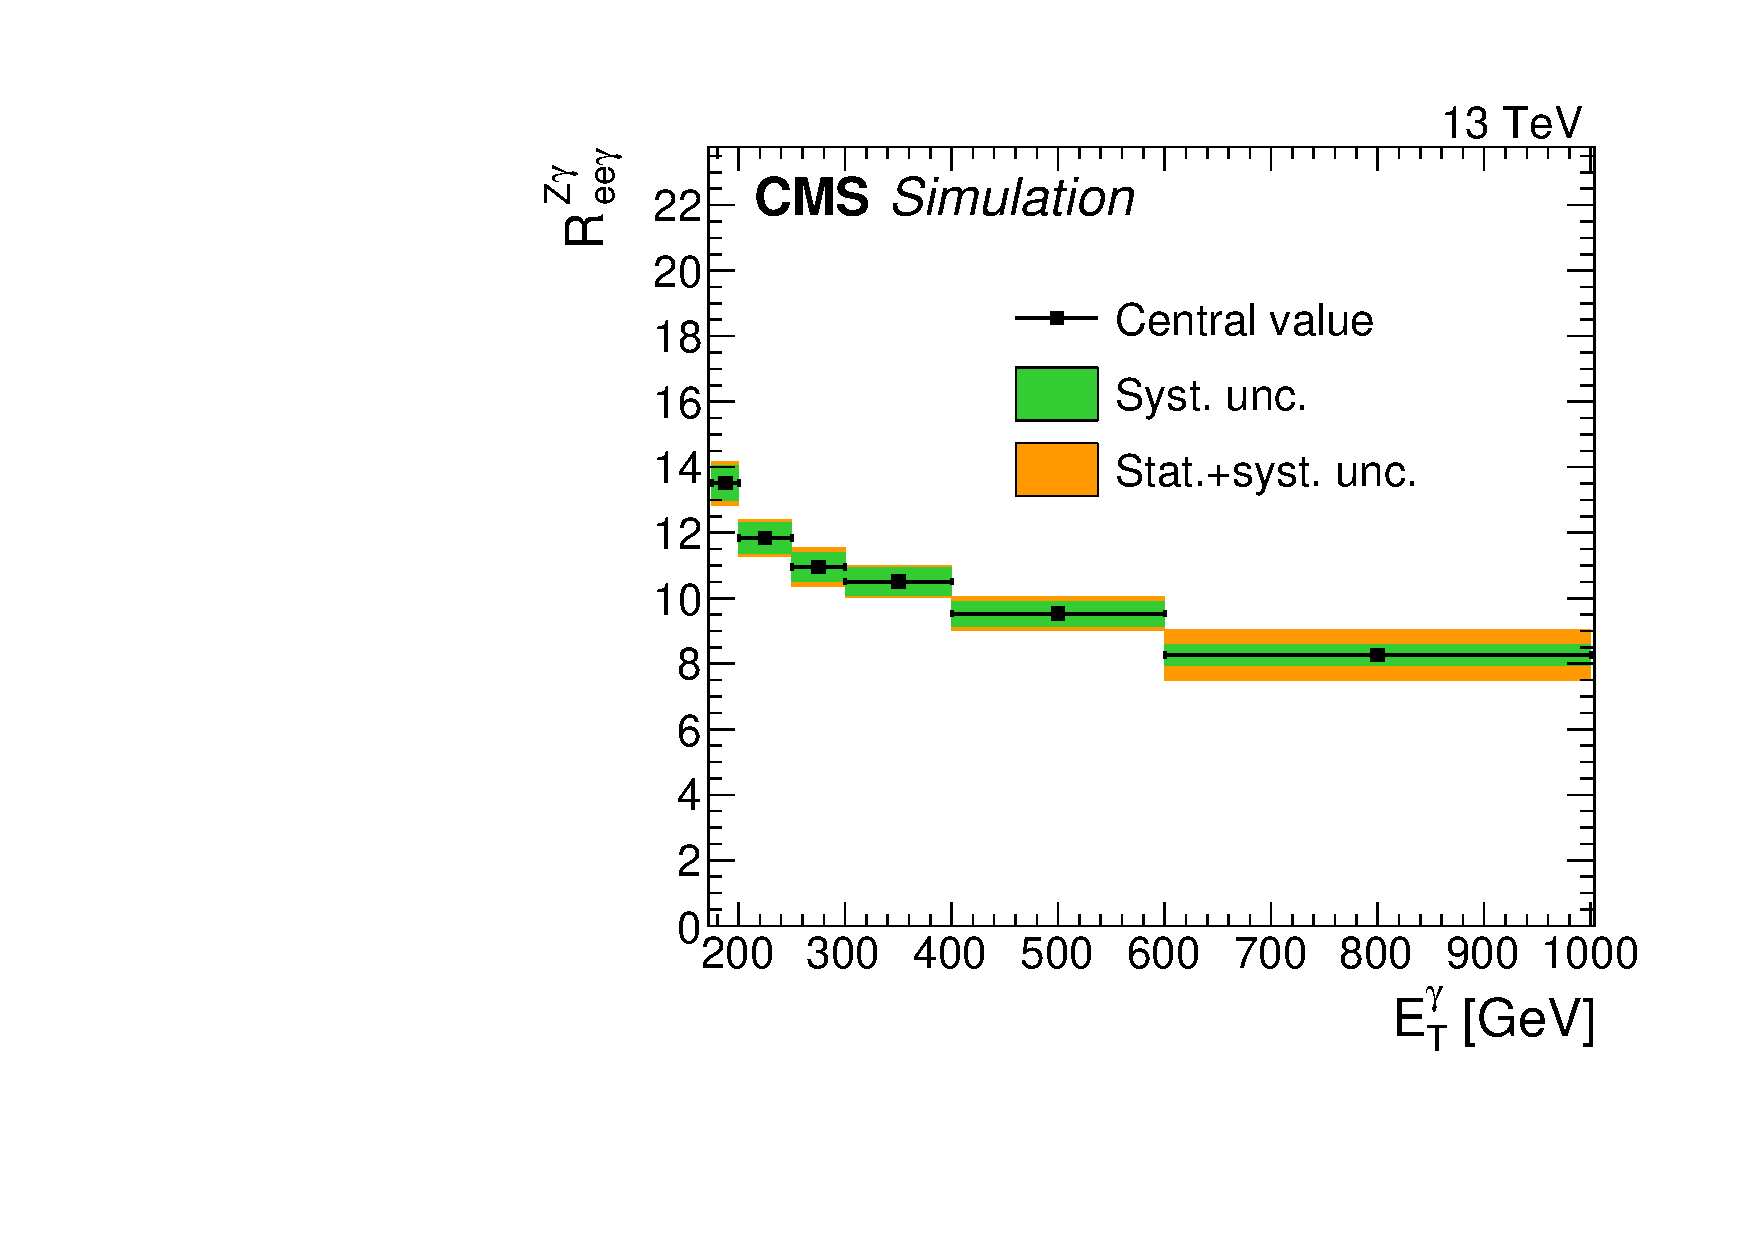
\includegraphics[width=0.49\textwidth]{Analysis/Figures/RZee.pdf}
    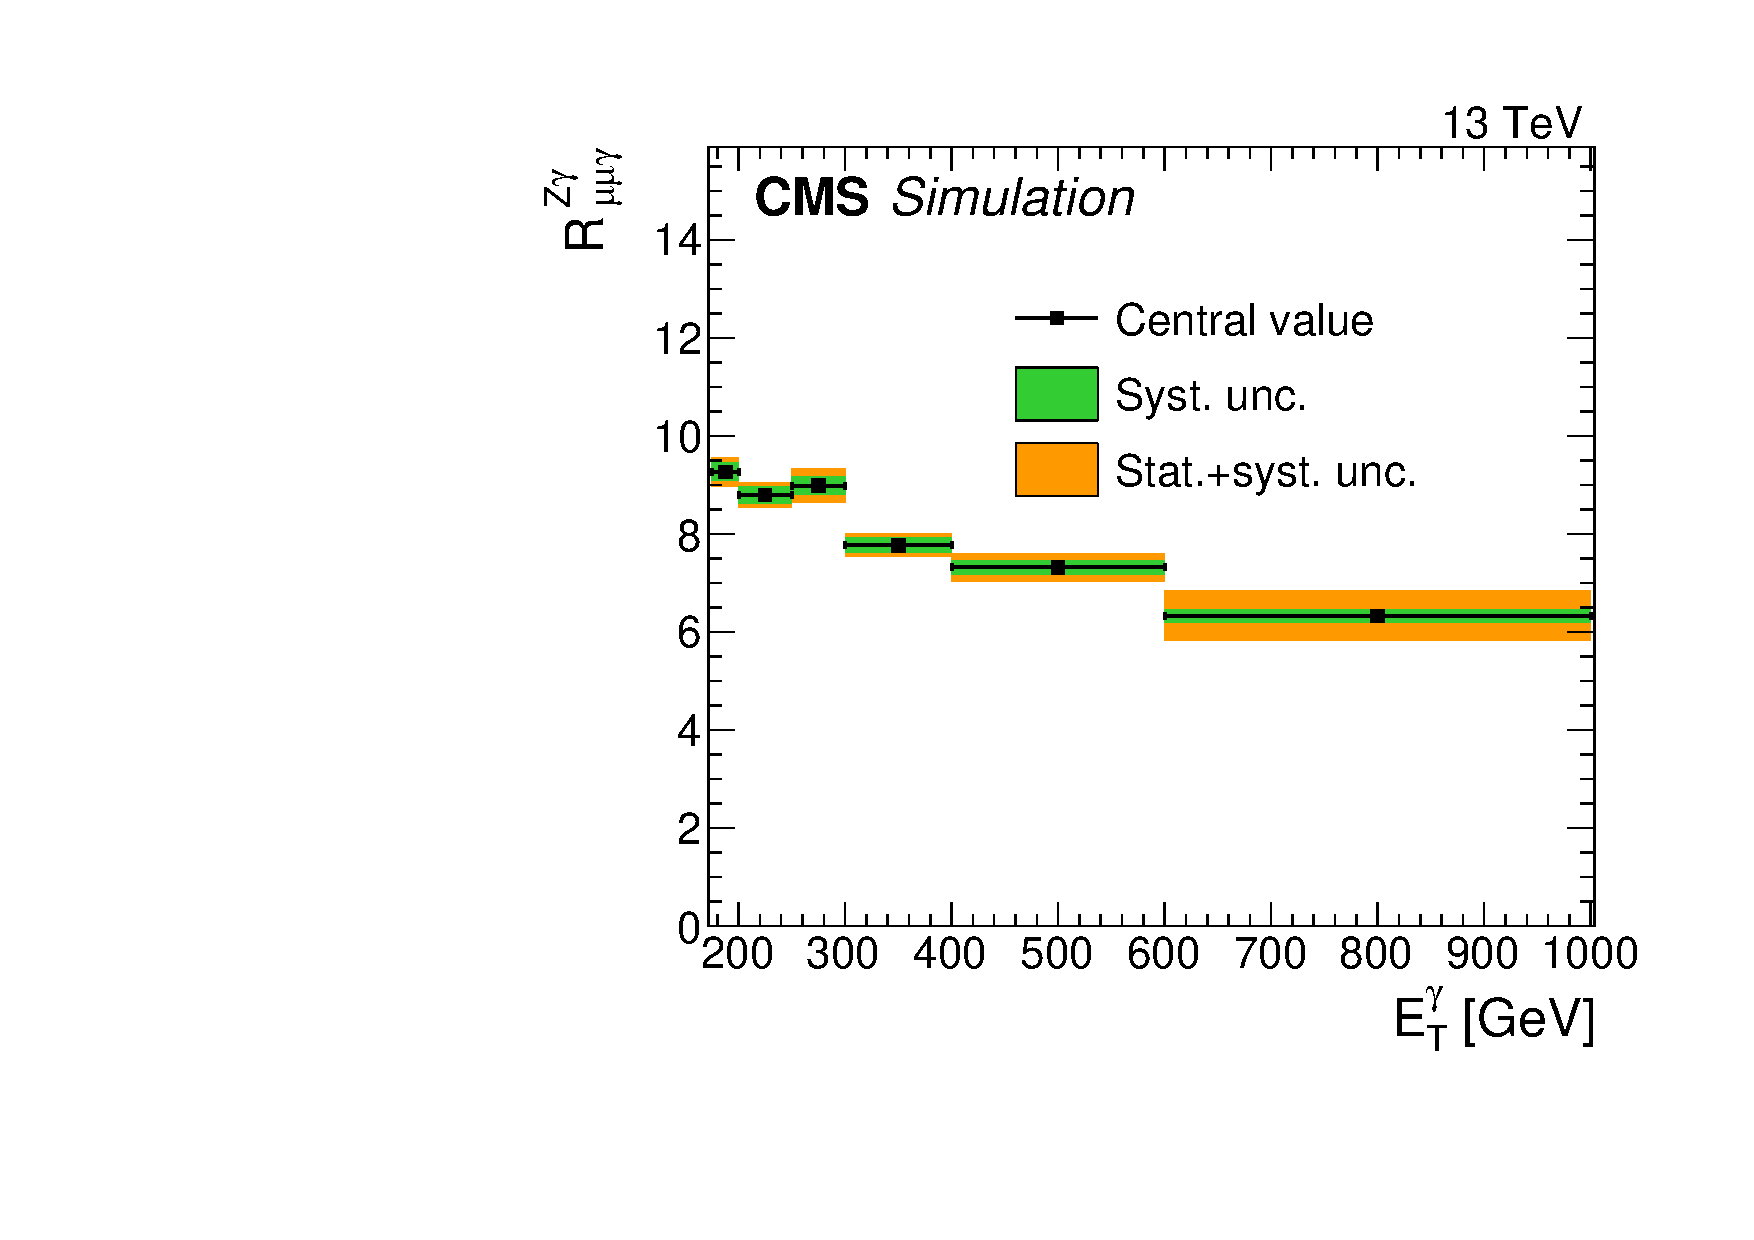
\includegraphics[width=0.49\textwidth]{Analysis/Figures/RZmm.pdf}
    \caption{
      Transfer factors \RZee\ (left) and \RZmm\ (right). 
      The uncertainty bands in green (inner) and orange (outer) show the systematic uncertainty, and the combination of systematic and statistical uncertainty arising from limited MC sample size, respectively. 
      The systematic uncertainties considered are the uncertainties in the data-to-simulation correction factors $\rho$ for the lepton identification efficiencies.
    }
    \label{fig:tf_z}
\end{figure}

Using the transfer factor \RZll, the total estimated event yield \Tll\ in each dilepton control region in the $i^\mathrm{th}$ bin of the \ETg\ distribution can be expressed as
\begin{equation}
  \Tll[,i] = \frac{\NZg[i]}{\RZll[,i]} + b_{\ell\ell\Pgg,i},
\end{equation}
where \NZg\ is the number of \zinvg\ events in the combined signal regions and $b_{\ell\ell\Pgg}$ is the predicted contribution from other background sources in the dilepton control region, namely \ttg, VV\Pgg, and misidentified hadrons. 
The subscript $i$ indicates that the quantities are evaluated in bin $i$ of the \ETg\ distribution.

\begin{figure}[htbp]
  \centering
    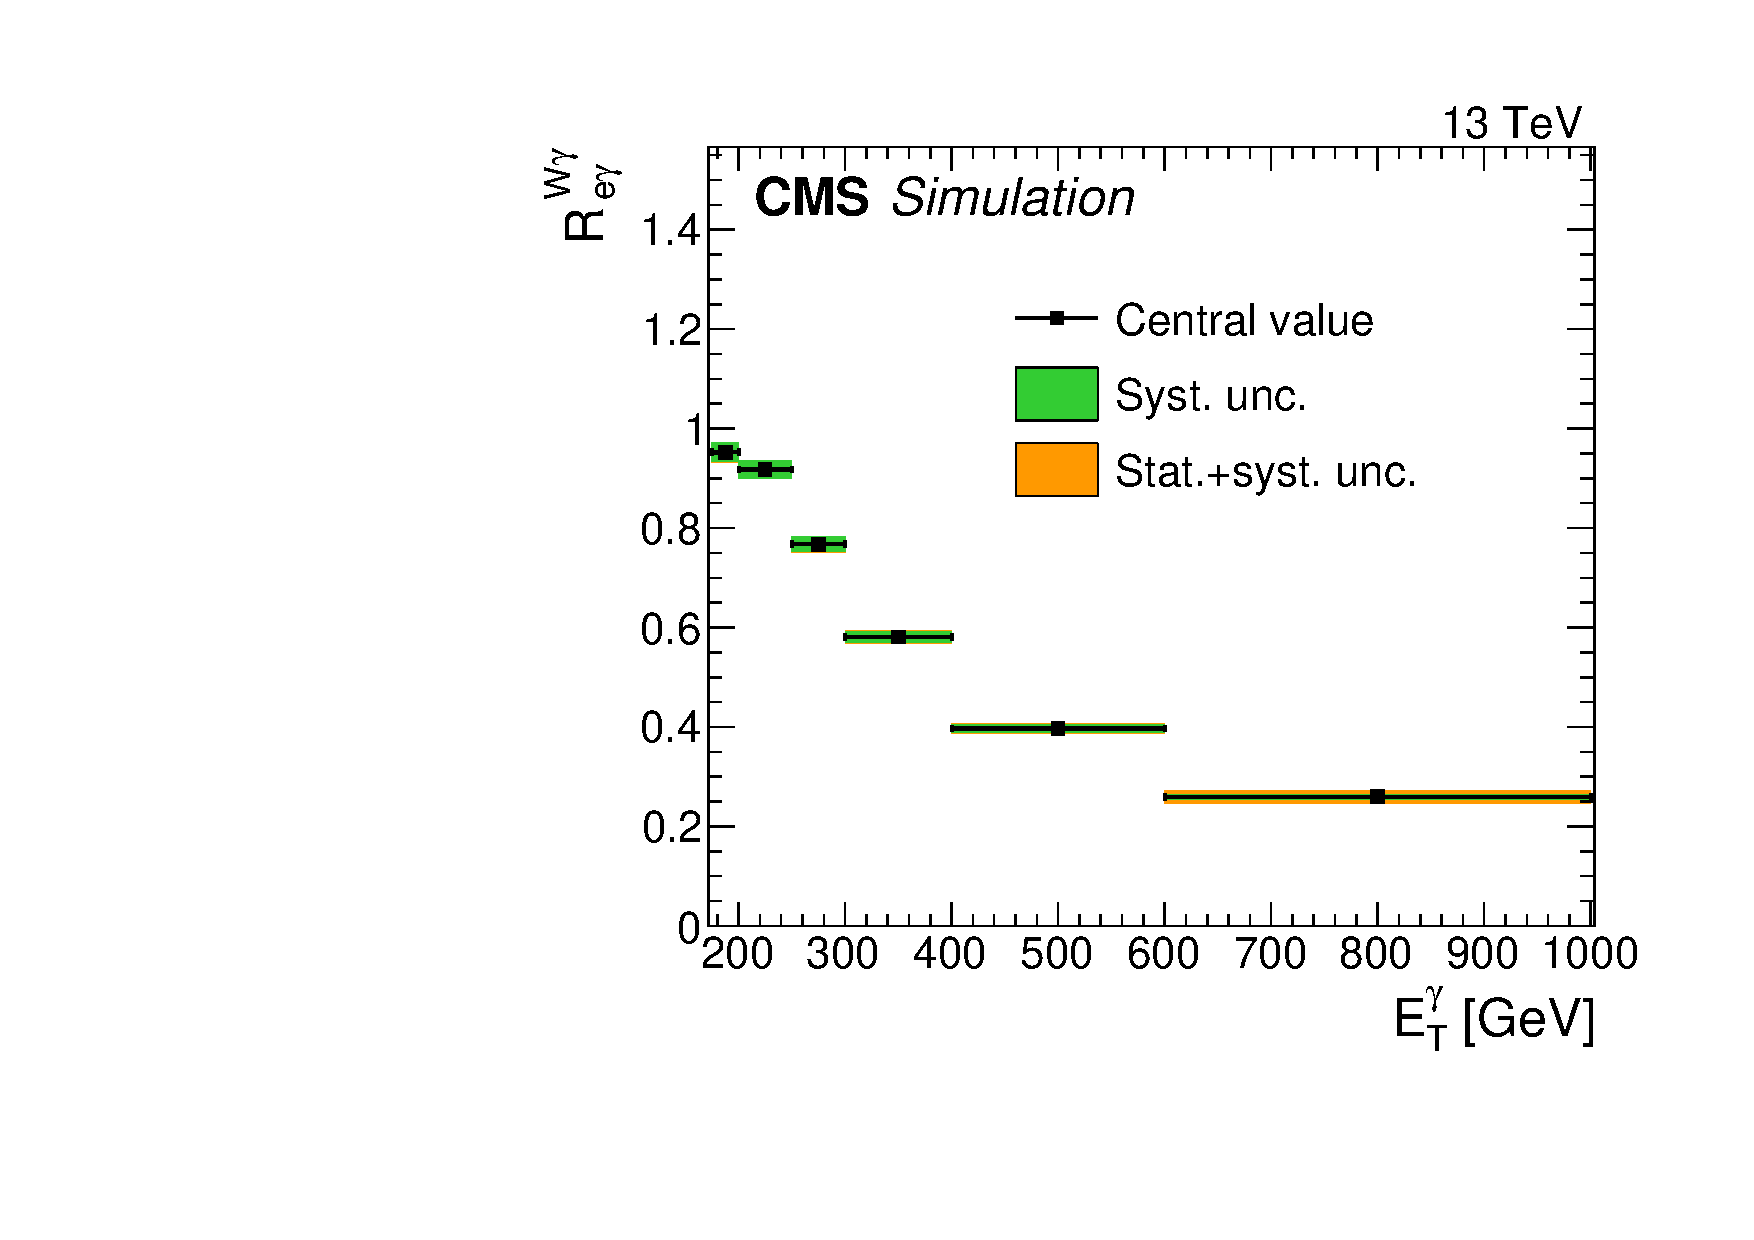
\includegraphics[width=0.49\textwidth]{Analysis/Figures/RWe.pdf}
    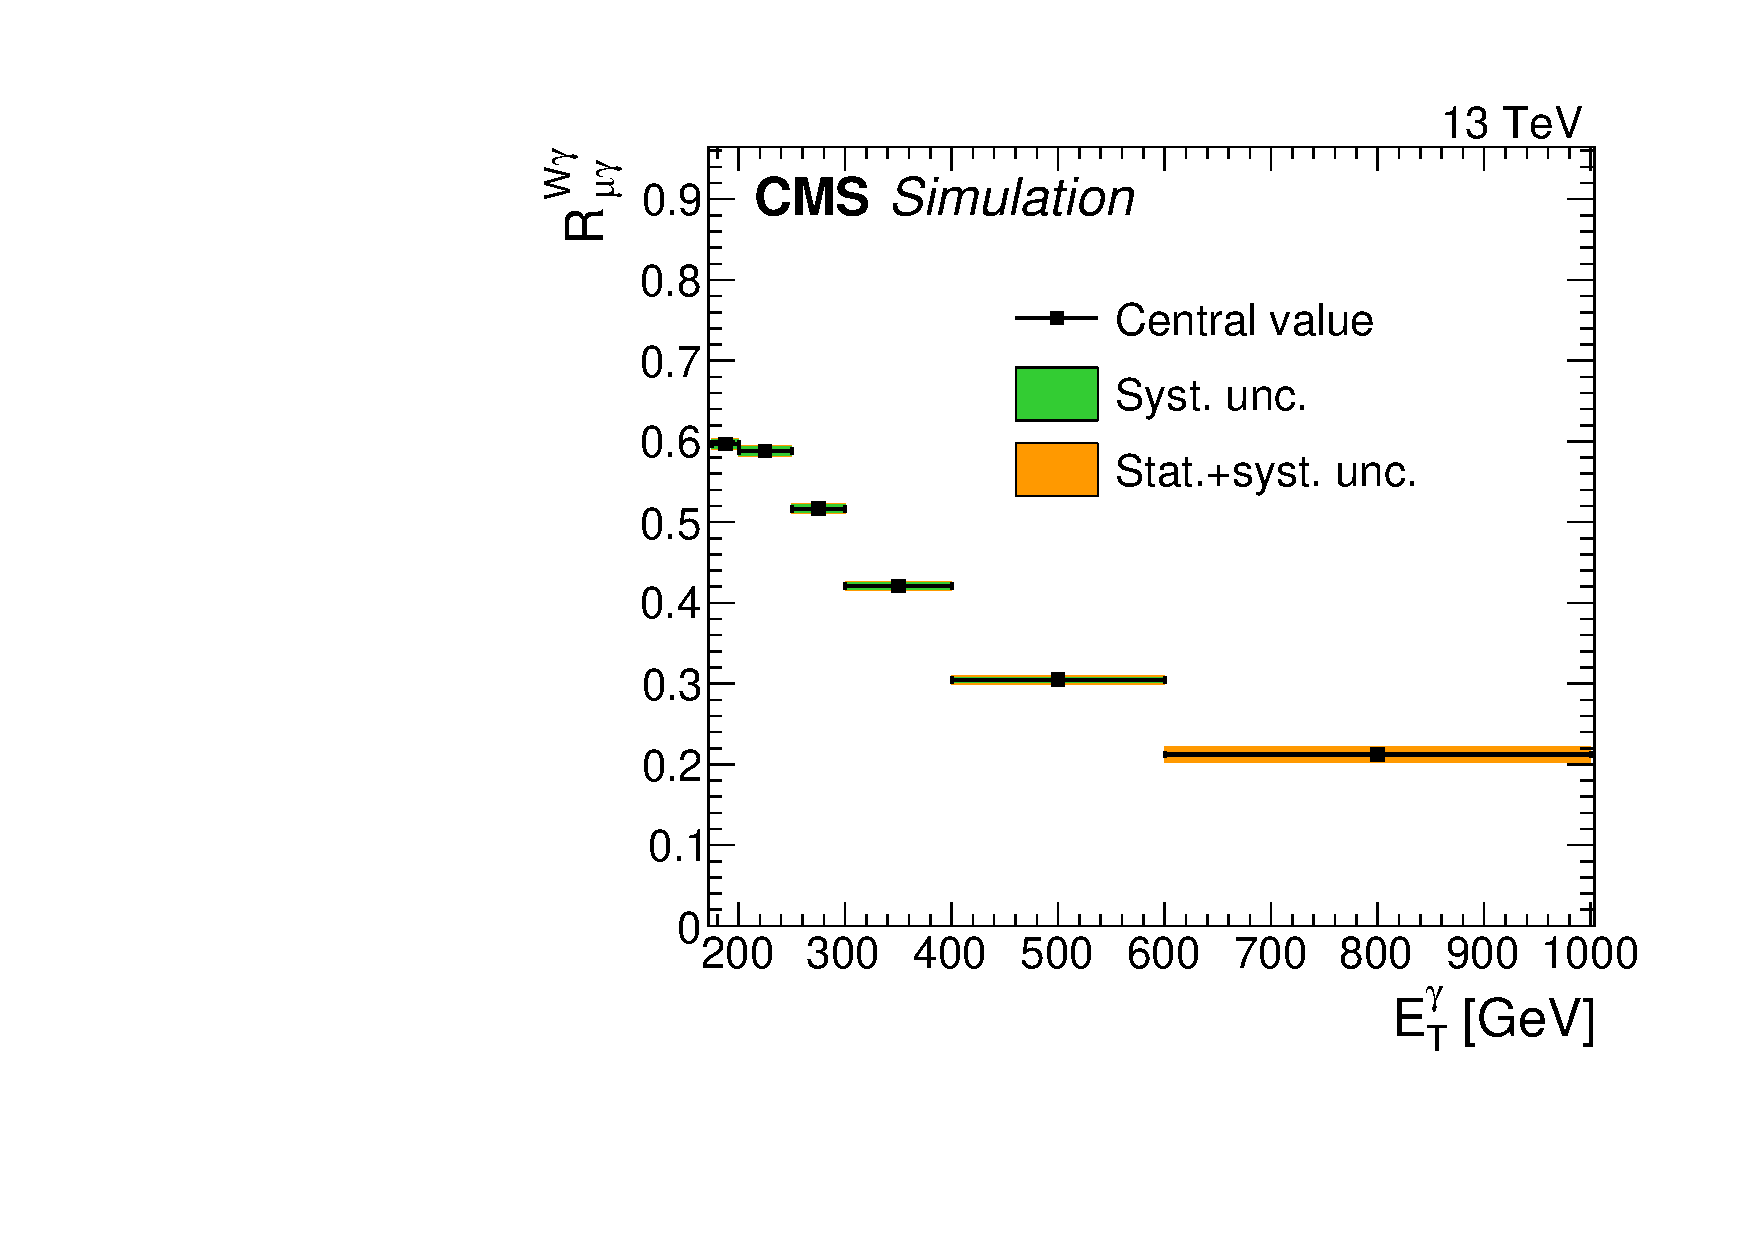
\includegraphics[width=0.49\textwidth]{Analysis/Figures/RWm.pdf}
    \caption{
      Transfer factors \RWe\ (left) and \RWm\ (right). 
      The uncertainty bands in green (inner) and orange (outer) show the systematic uncertainty, and the combination of systematic and statistical uncertainty arising from limited MC sample size, respectively. 
      The systematic uncertainties considered are the uncertainties in the data-to-simulation correction factors $\rho$ for the lepton identification efficiencies.
    }
    \label{fig:tf_w}
\end{figure}

\begin{figure}[htbp]
  \centering
    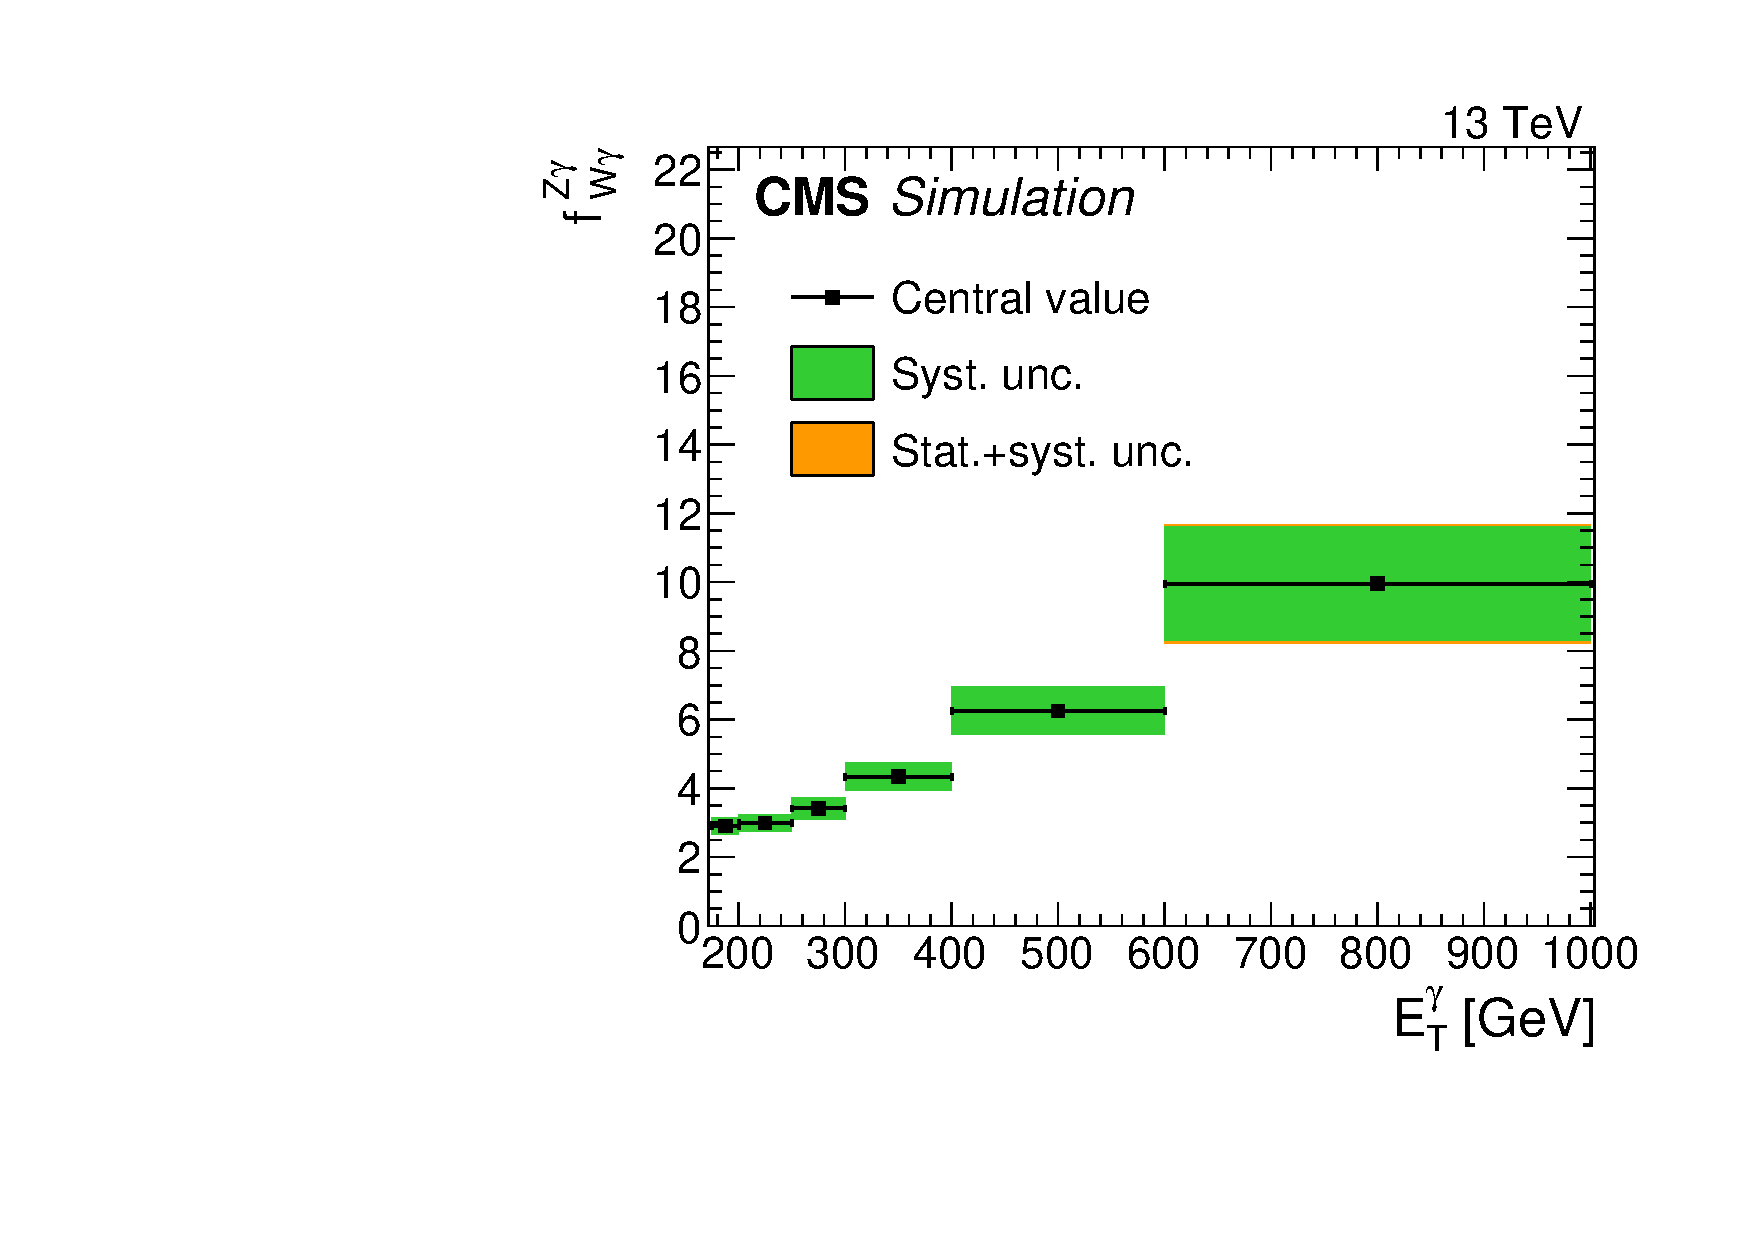
\includegraphics[width=0.49\textwidth]{Analysis/Figures/fZW.pdf}
    \caption{
      Transfer factor \fZW. 
      The uncertainty bands in green (inner) and orange (outer) show the systematic uncertainty, and the combination of systematic and statistical uncertainty arising from limited MC sample size, respectively. 
      The systematic uncertainties considered are the uncertainties from higher-order theoretical corrections.
    }
    \label{fig:tf_wz}
\end{figure}

Using \RWl\ and \fZW, the total estimated event yield \Tl\ in each single-lepton control region in the $i^\mathrm{th}$ bin of the \ETg\ distribution can be expressed as
\begin{equation}
  \Tl[,i] = \frac{\NZg[i]}{\RWl[,i]\fZW[,i]} + b_{\ell\Pgg,i},
\end{equation}
where $b_{\ell\Pgg}$ is the predicted contribution from other background sources in the single-lepton regions, namely misidentified electrons and hadrons and other minor SM processes.

\subsection{Higher-order corrections to \vg\ differential cross sections}
\label{sec:theory_uncertainties}

\begin{figure}[htbp]
  \centering
  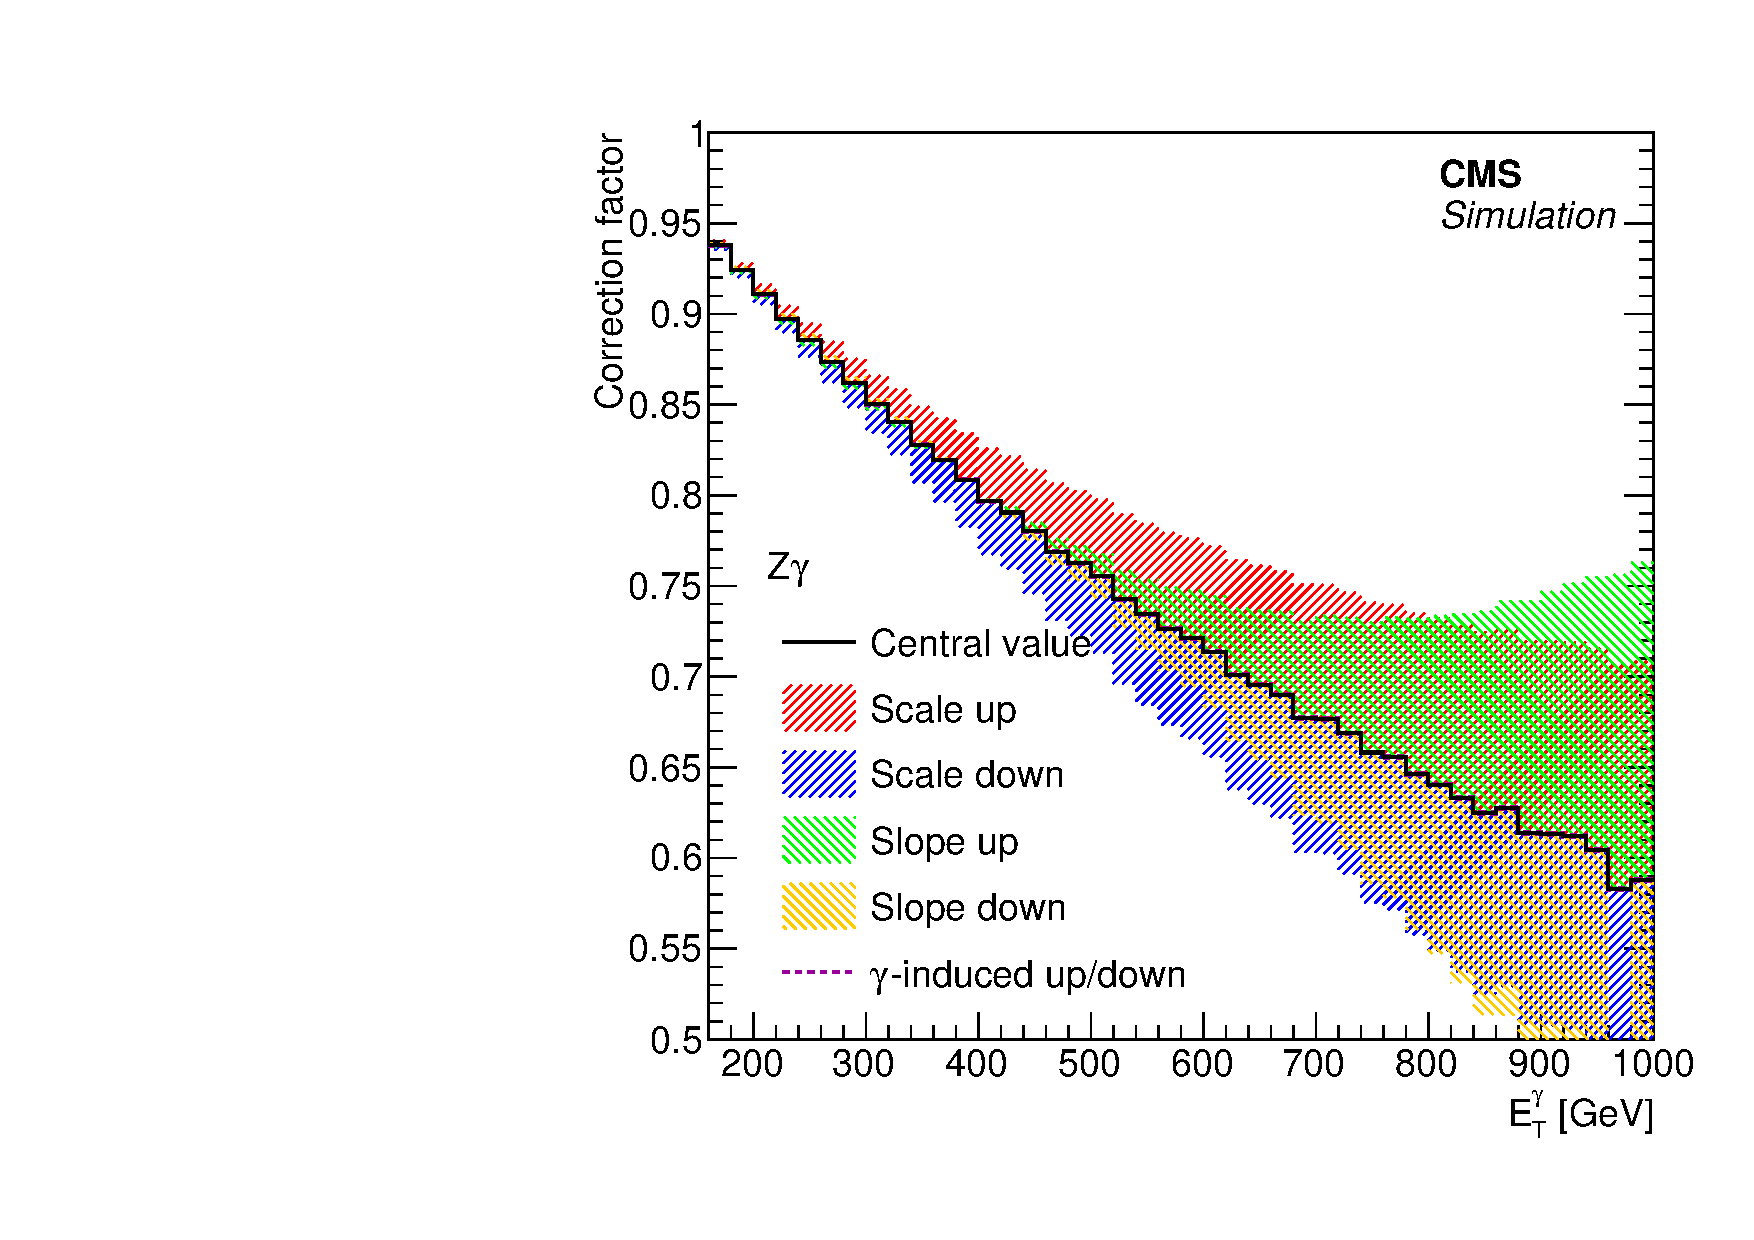
\includegraphics[width=0.48\linewidth]{Analysis/Figures/ewkcorr_zg.pdf} \\
  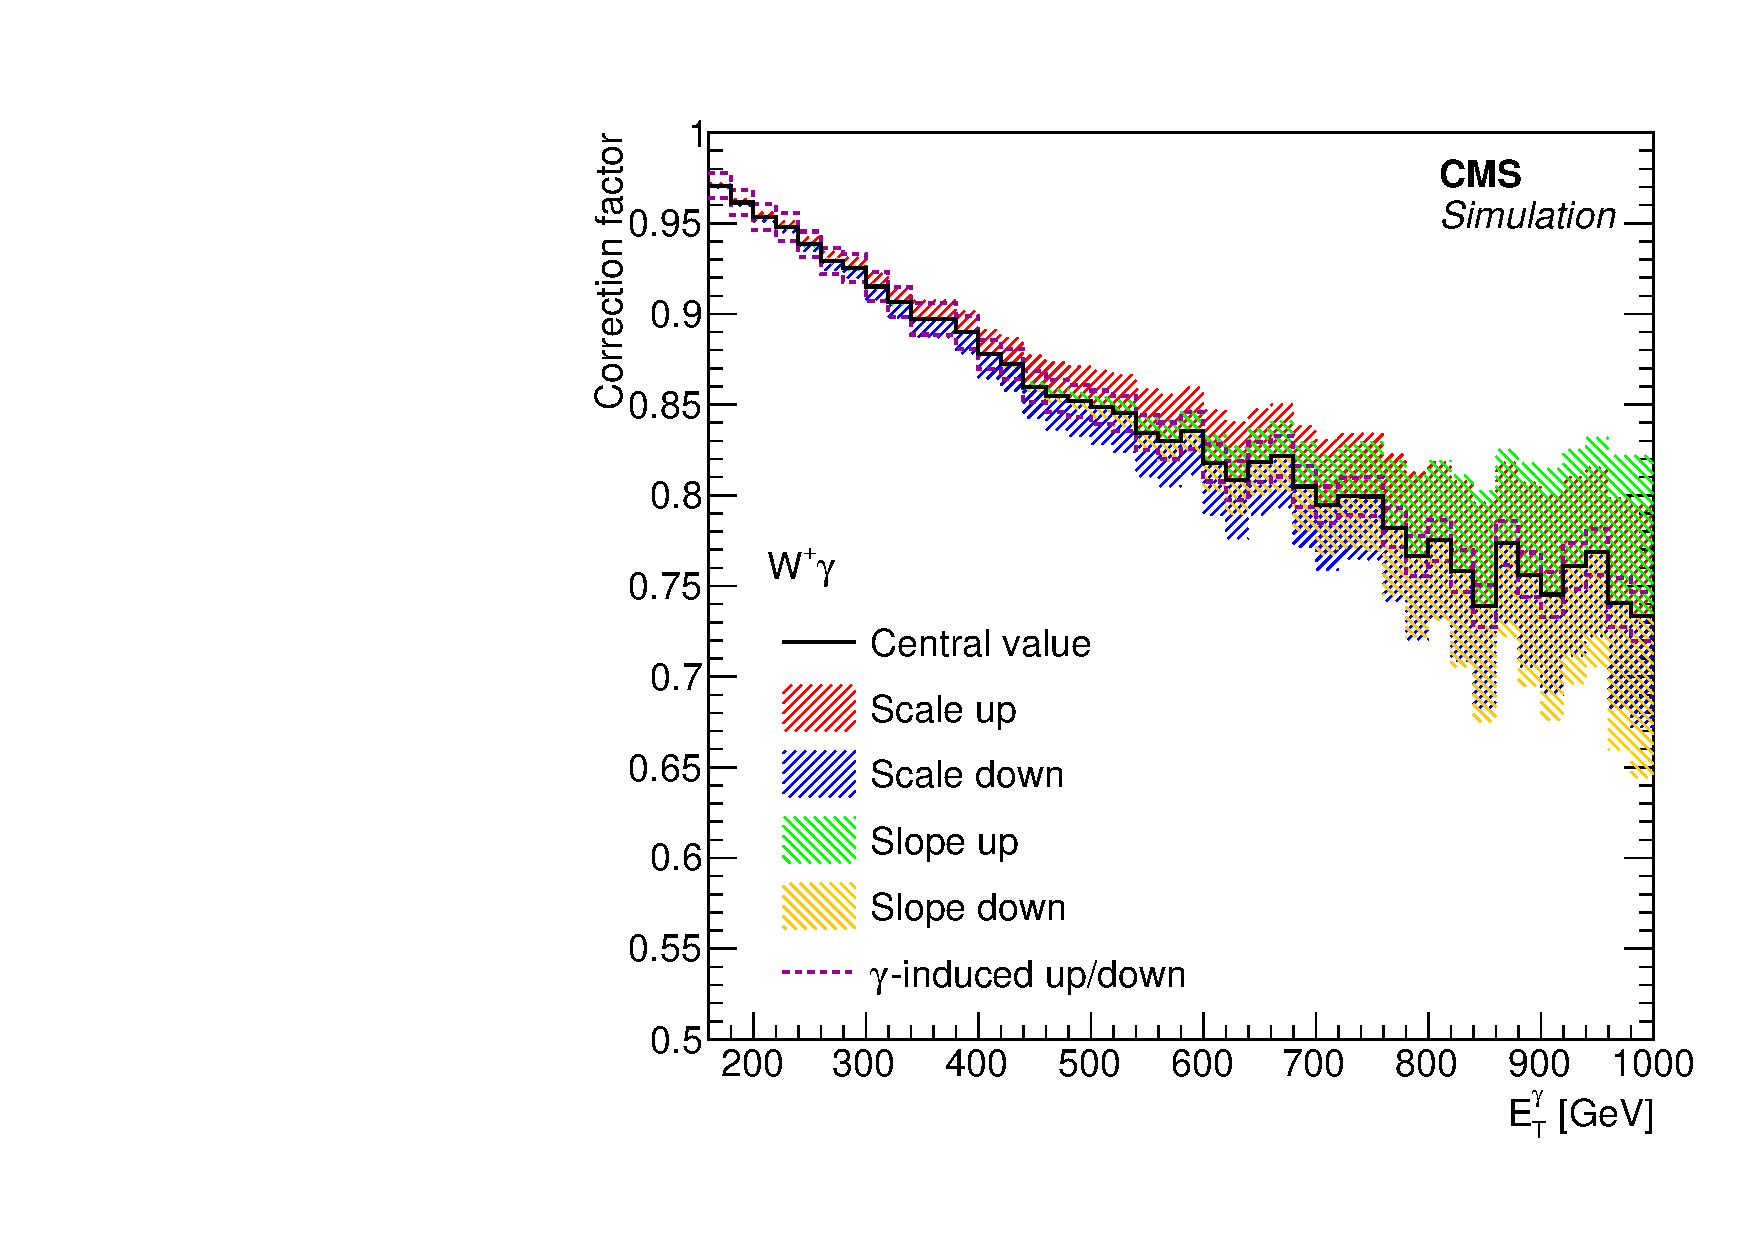
\includegraphics[width=0.48\linewidth]{Analysis/Figures/ewkcorr_wgplus.pdf}
  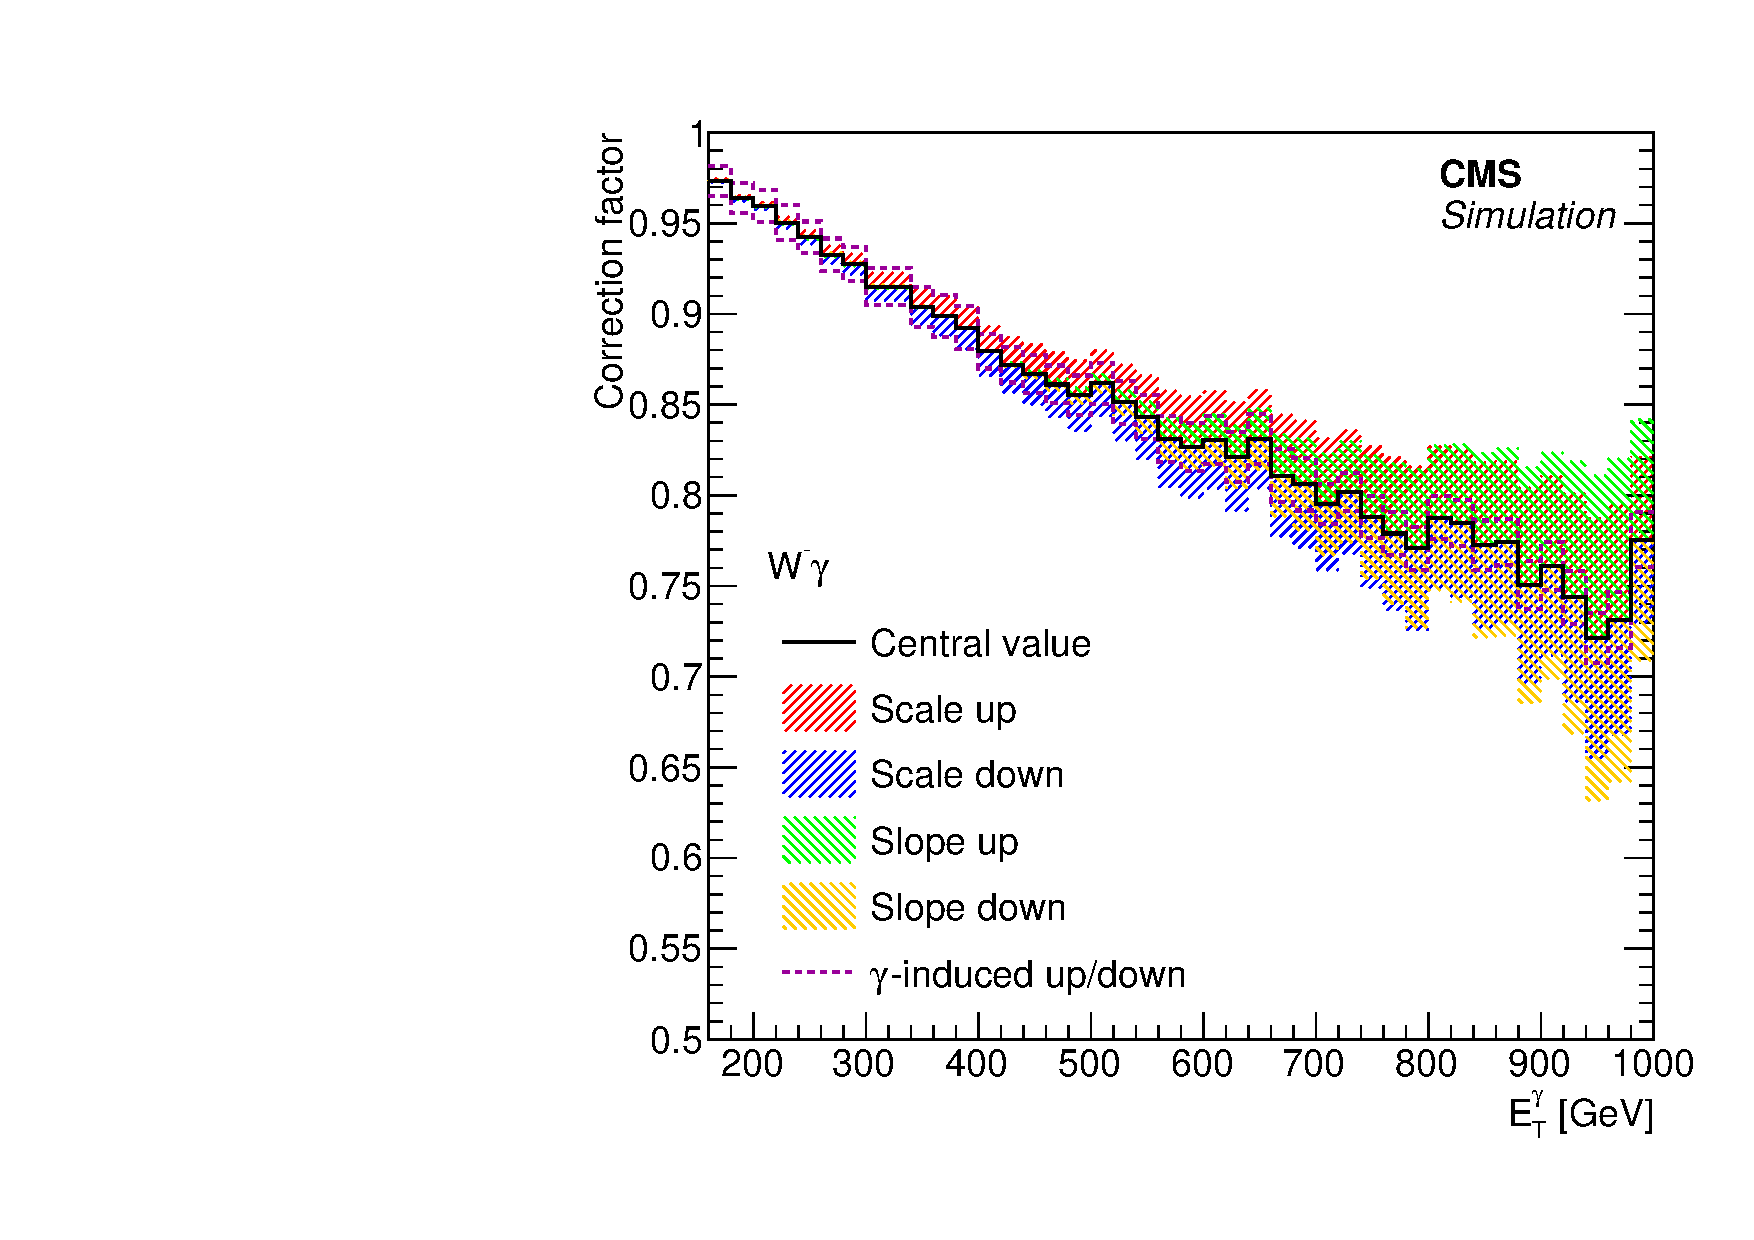
\includegraphics[width=0.48\linewidth]{Analysis/Figures/ewkcorr_wgminus.pdf}
  \caption{
    Electroweak NLO cross section corrections as a function of photon \pt\ for \zinvg\ (top), $\PW^{+}+\Pgg$ (bottom left), and $\PW^{-}+\Pgg$ (bottom right) processes, overlaid with uncertainty bands. 
    See text for descriptions of the individual components of the uncertainty.
    The uncertainty due to \Pgg-induced production is negligible in \zinvg\ production.
  }
  \label{fig:ewk_correction}
\end{figure}

We apply the correction factors shown in Fig.~\ref{fig:ewk_correction}, which are combinations of Sudakov suppression factors and photon-induced enhancements, and are provided by the authors of Ref.~\cite{Denner:2015fca} in addition to the NNLO QCD correction.

\begin{figure}[htbp]
  \centering
    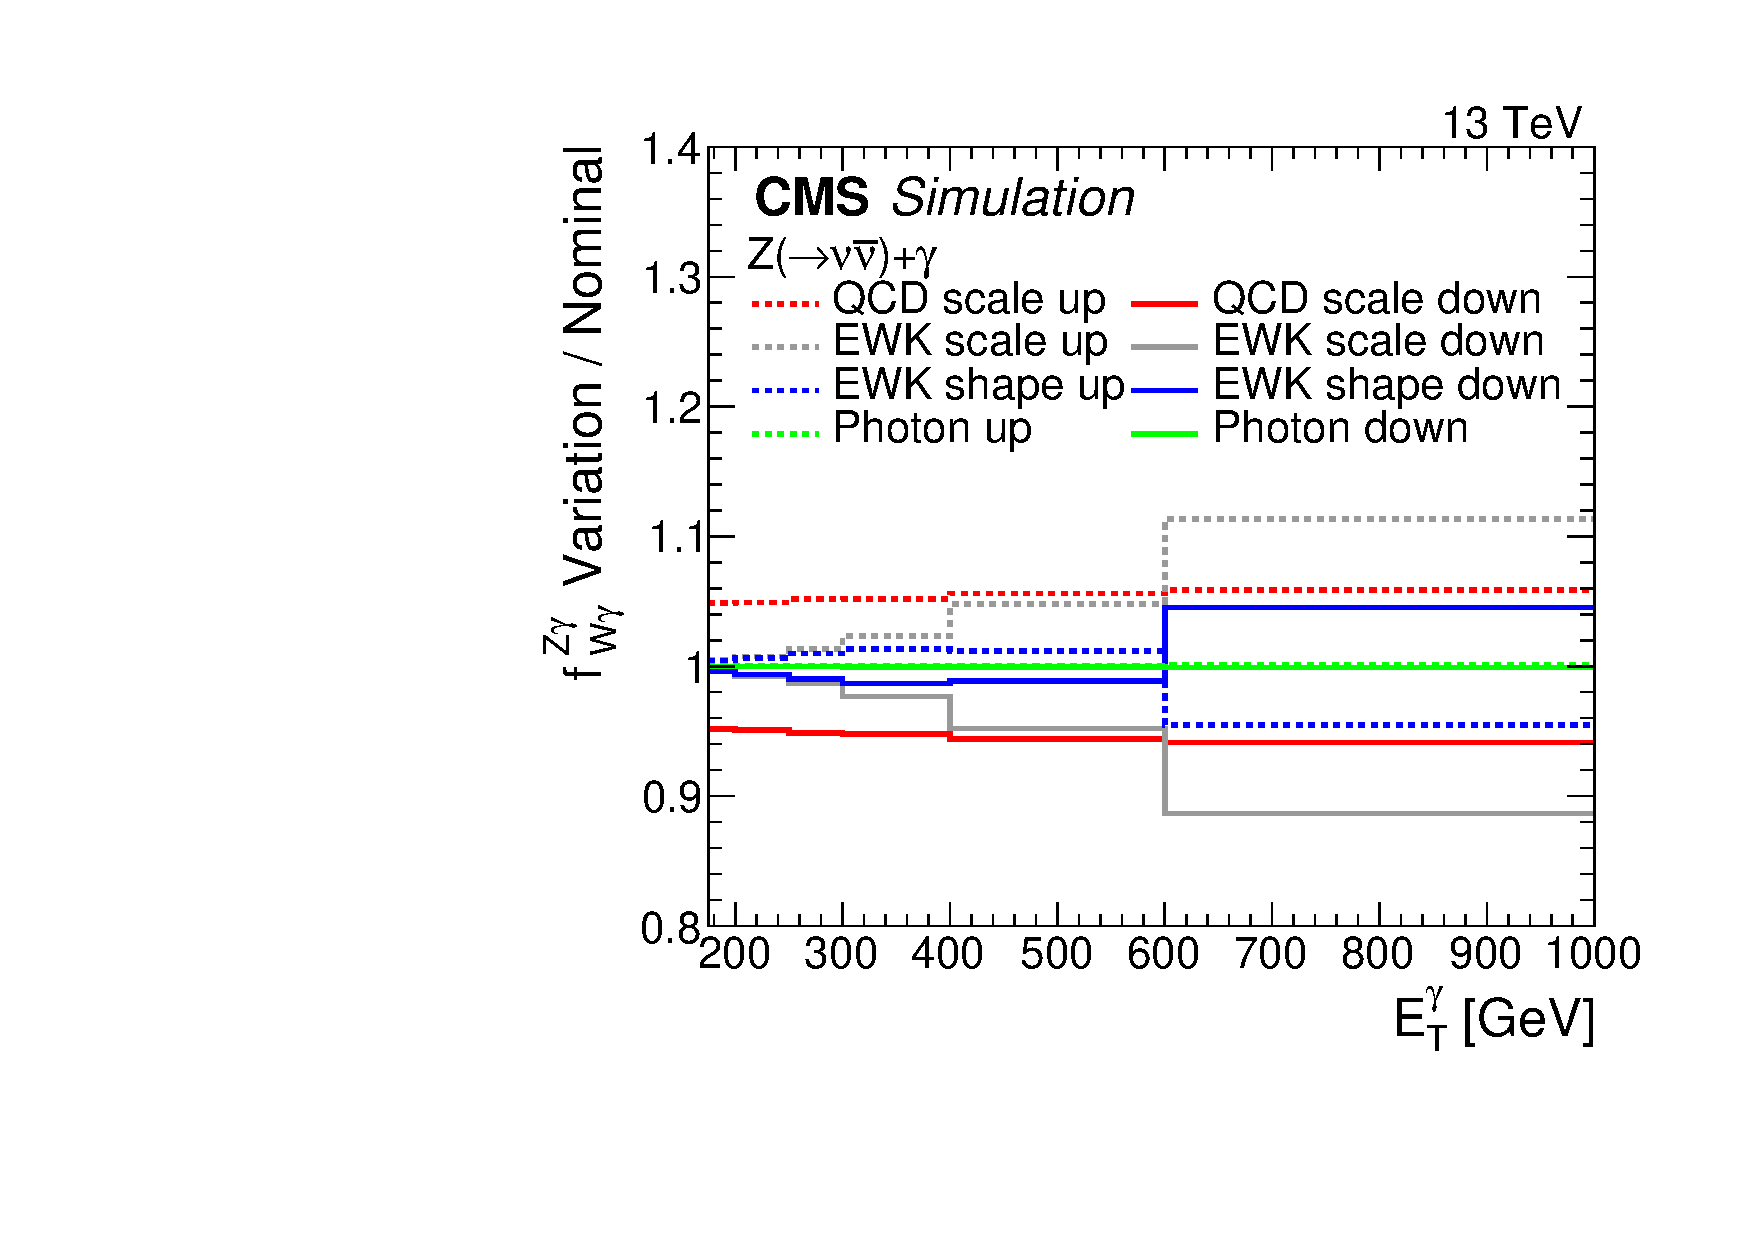
\includegraphics[width=0.45\textwidth]{Analysis/Figures/tf_syst_zg.pdf}
    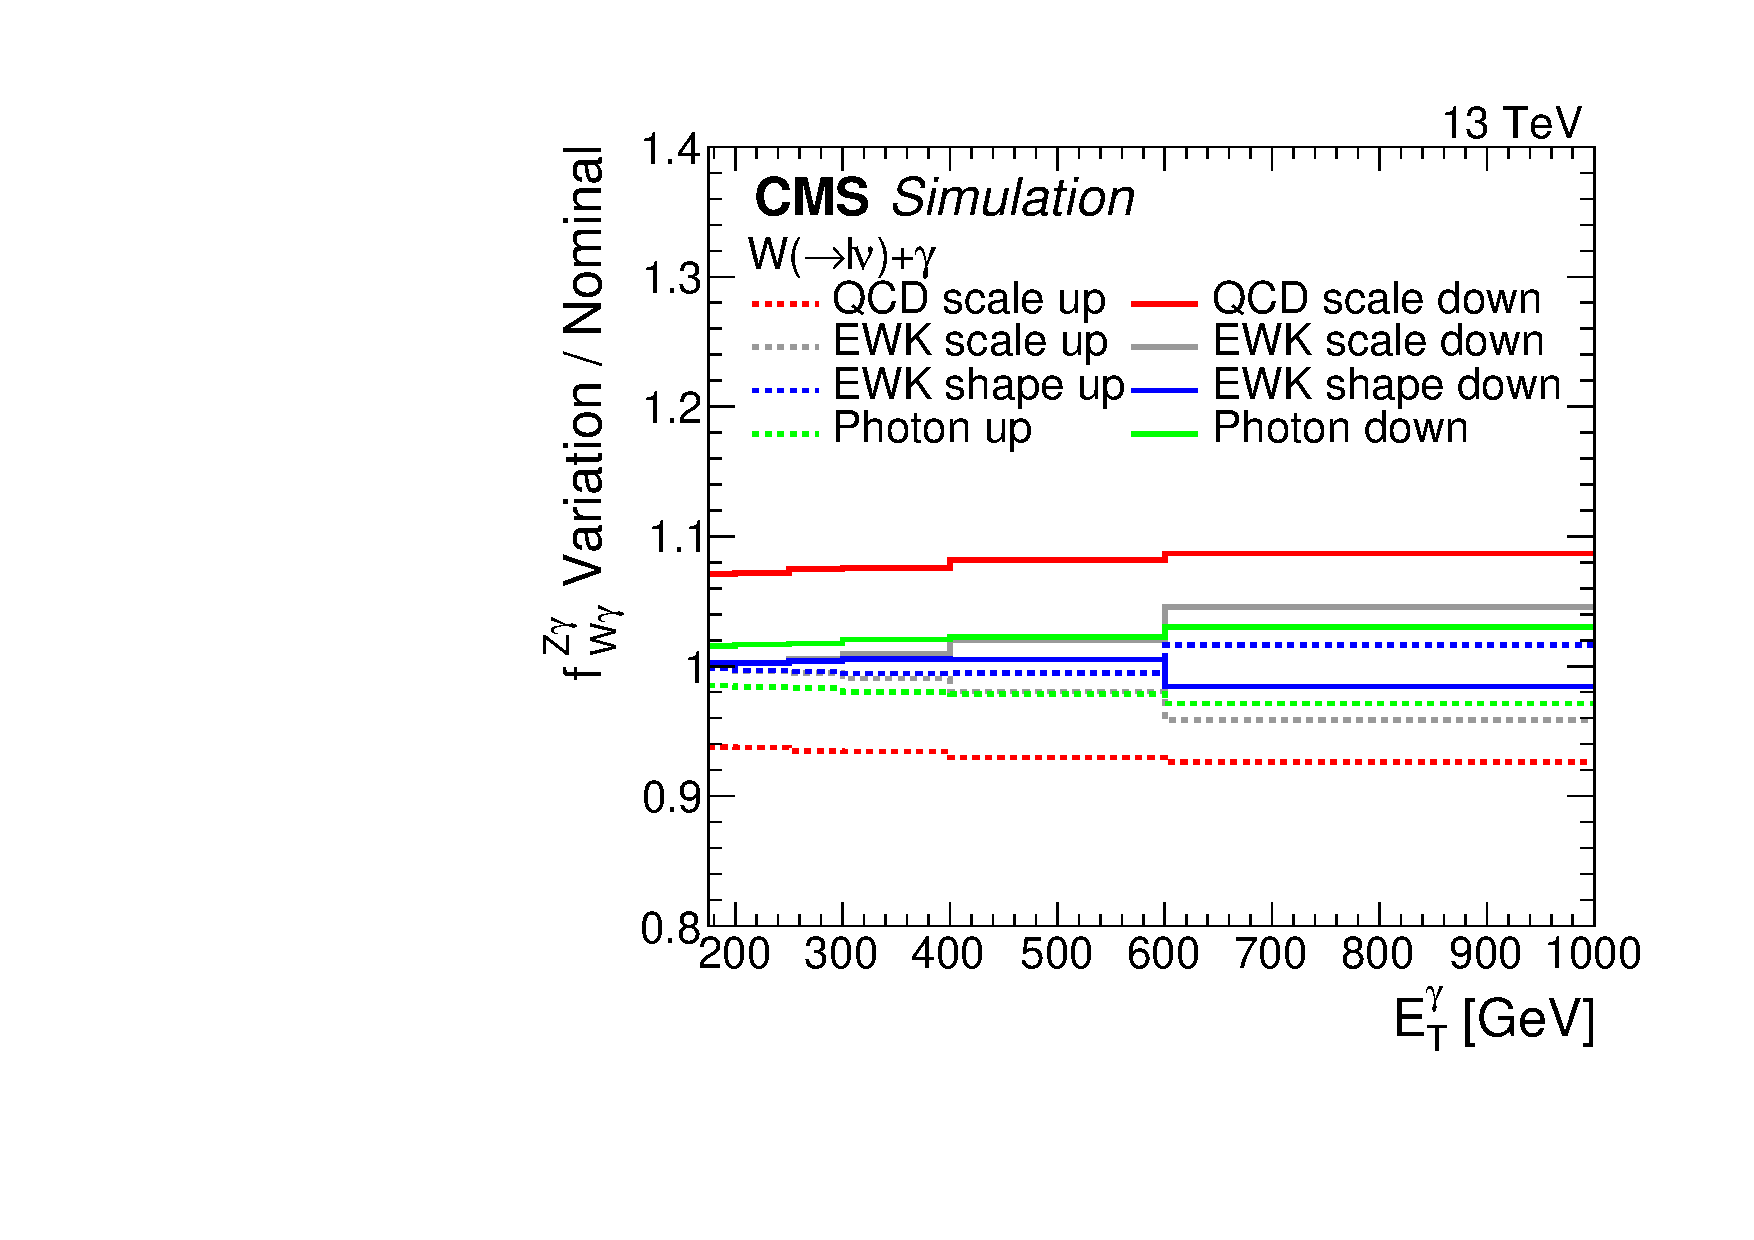
\includegraphics[width=0.45\textwidth]{Analysis/Figures/tf_syst_wg.pdf}
    \caption{
      Systematic uncertainty in the transfer factors for \zinvg\ (left) and \wlng\ (right). The last bin includes all events with $\ETg > 1000\GeV$.
    }
    \label{fig:tf_syst}
\end{figure}

Figure~\ref{fig:tf_syst} shows the effect of systematic uncertainty in the ratio between the \zinvg\ and \wlng\ processes with respect to nominal value for \PZ\Pgg\ and \PW\Pgg\ respectively.

\section{Misidentified electrons}
\label{sec:efake}

An electron can be misidentified as a photon if the association of tracks or track seeds to the supercluster in ECAL fails in the reconstruction step. 
The production of a single \PW\ boson decaying to an electron and a neutrino is a high-rate process, and it mimicks the photon plus \met\ signature if the electron is misidentified.

The rate at which this misidentification occurs is proportional to the inefficiency $1 - \epsilon_{\Pe}^{\text{track}}$ of the tracking, defined over the electrons passing the photon identification criteria described in Sec.~\ref{sec:photons} except the electron veto. 
This partial identification is denoted as \Pe\Pgg\ ID in the following.  
If one assumes that the kinematic and other critical properties of the electron plus \met\ events are unaffected by the electron misidentification, it is possible to model the electron misidentification background by taking a proxy sample with well-identified electrons and scaling this sample by $R_{\Pe} = (1 - \epsilon_{\Pe}^{\text{track}}) / \epsilon_{\Pe}^{\text{track}}$.

The ``tag-and-probe'' method described in Section~\ref{subsec:idsf} with appropriate changes is used to measure the efficiency corresponding to the factor $R_{\Pe}$ in data.

The first such change is that the sample is split into \Pe\Pgg\ and \Pe\Pe\ categories depending on whether the probe passes or fails the electron veto requirement. 
Probes in both categories must also pass the \Pe\Pgg\ ID.
Denoting the area of the peak in each cateogry  $N_{\Pe\Pgg}$ and $N_{\Pe\Pe}$, respectively, the ratio $N_{\Pe\Pgg} / N_{\Pe\Pe}$ is equal to $R_{\Pe}$ up to minor systematic corrections.

The second such change is in the background model used in the TP fits. 
The backgrounds to the \Pe\Pgg\ fit consist of processes with actual electron and photon in the final state, such as \PW\Pgg\ and \Zee\ with a hard radiation off one of the electrons.
Because of this, we scale the mass distrubition of the $\Pgm+\Pgg$ sample by the ratio of electron-probe to muon-probe events taken from MC to account for the different rates of FSR and bremsstrahlung between muons and electrons.
As an alternative template to assess the systematic effect introduced by the choice of the background template, the unscaled mass distribution is also tested.

Figure~\ref{fig:efake_fits} shows the six fits performed on \Pe\Pe\ and \Pe\Pgg\ in bins of probe $\pt$, from which the $R_{\Pe}$ factor used for the estimation of the electron misidentification background is derived. 

%%% these fils have charged PF veto included, need to swap out
\begin{figure}[htbp]
  \begin{center}
    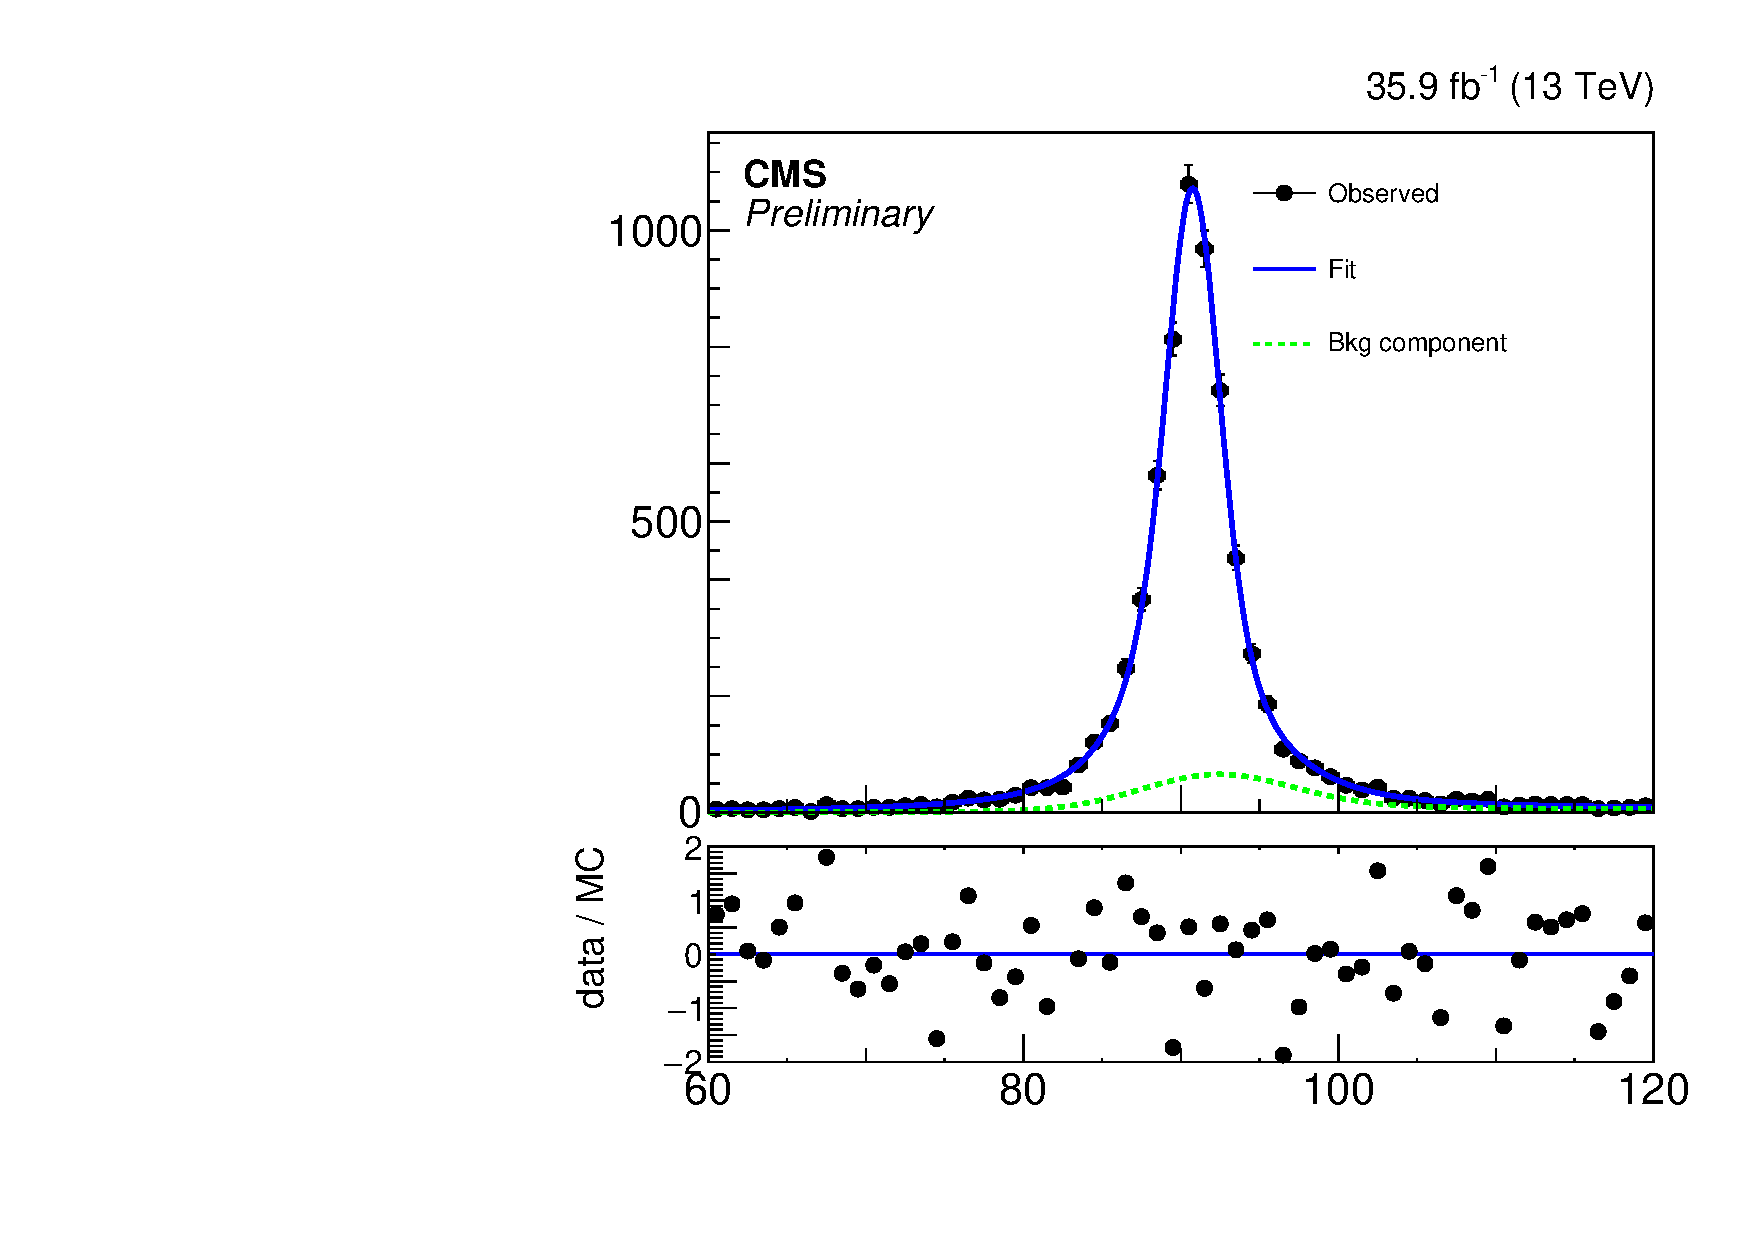
\includegraphics[width=0.48\linewidth]{Analysis/Figures/fit_data_ee_pt_175_200.pdf}
    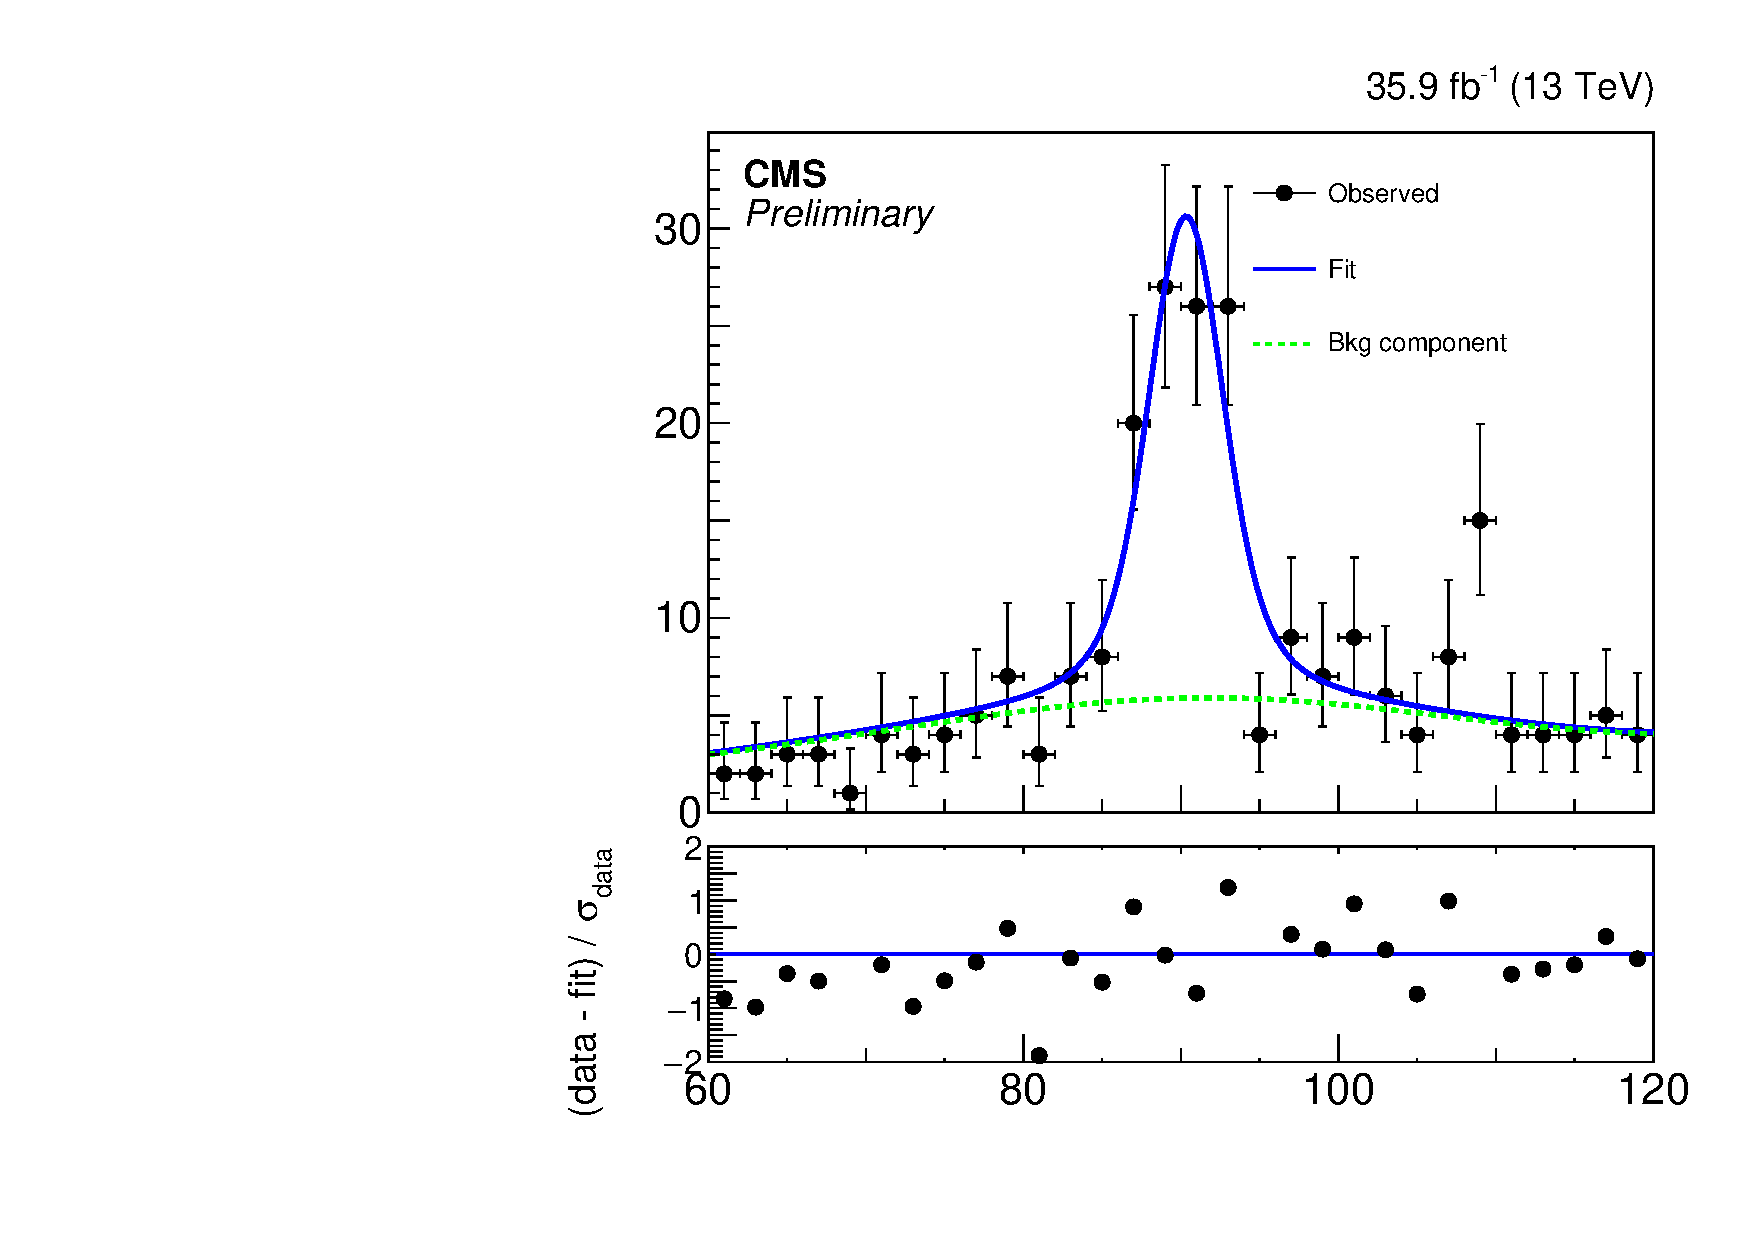
\includegraphics[width=0.48\linewidth]{Analysis/Figures/fit_data_eg_pt_175_200.pdf}
    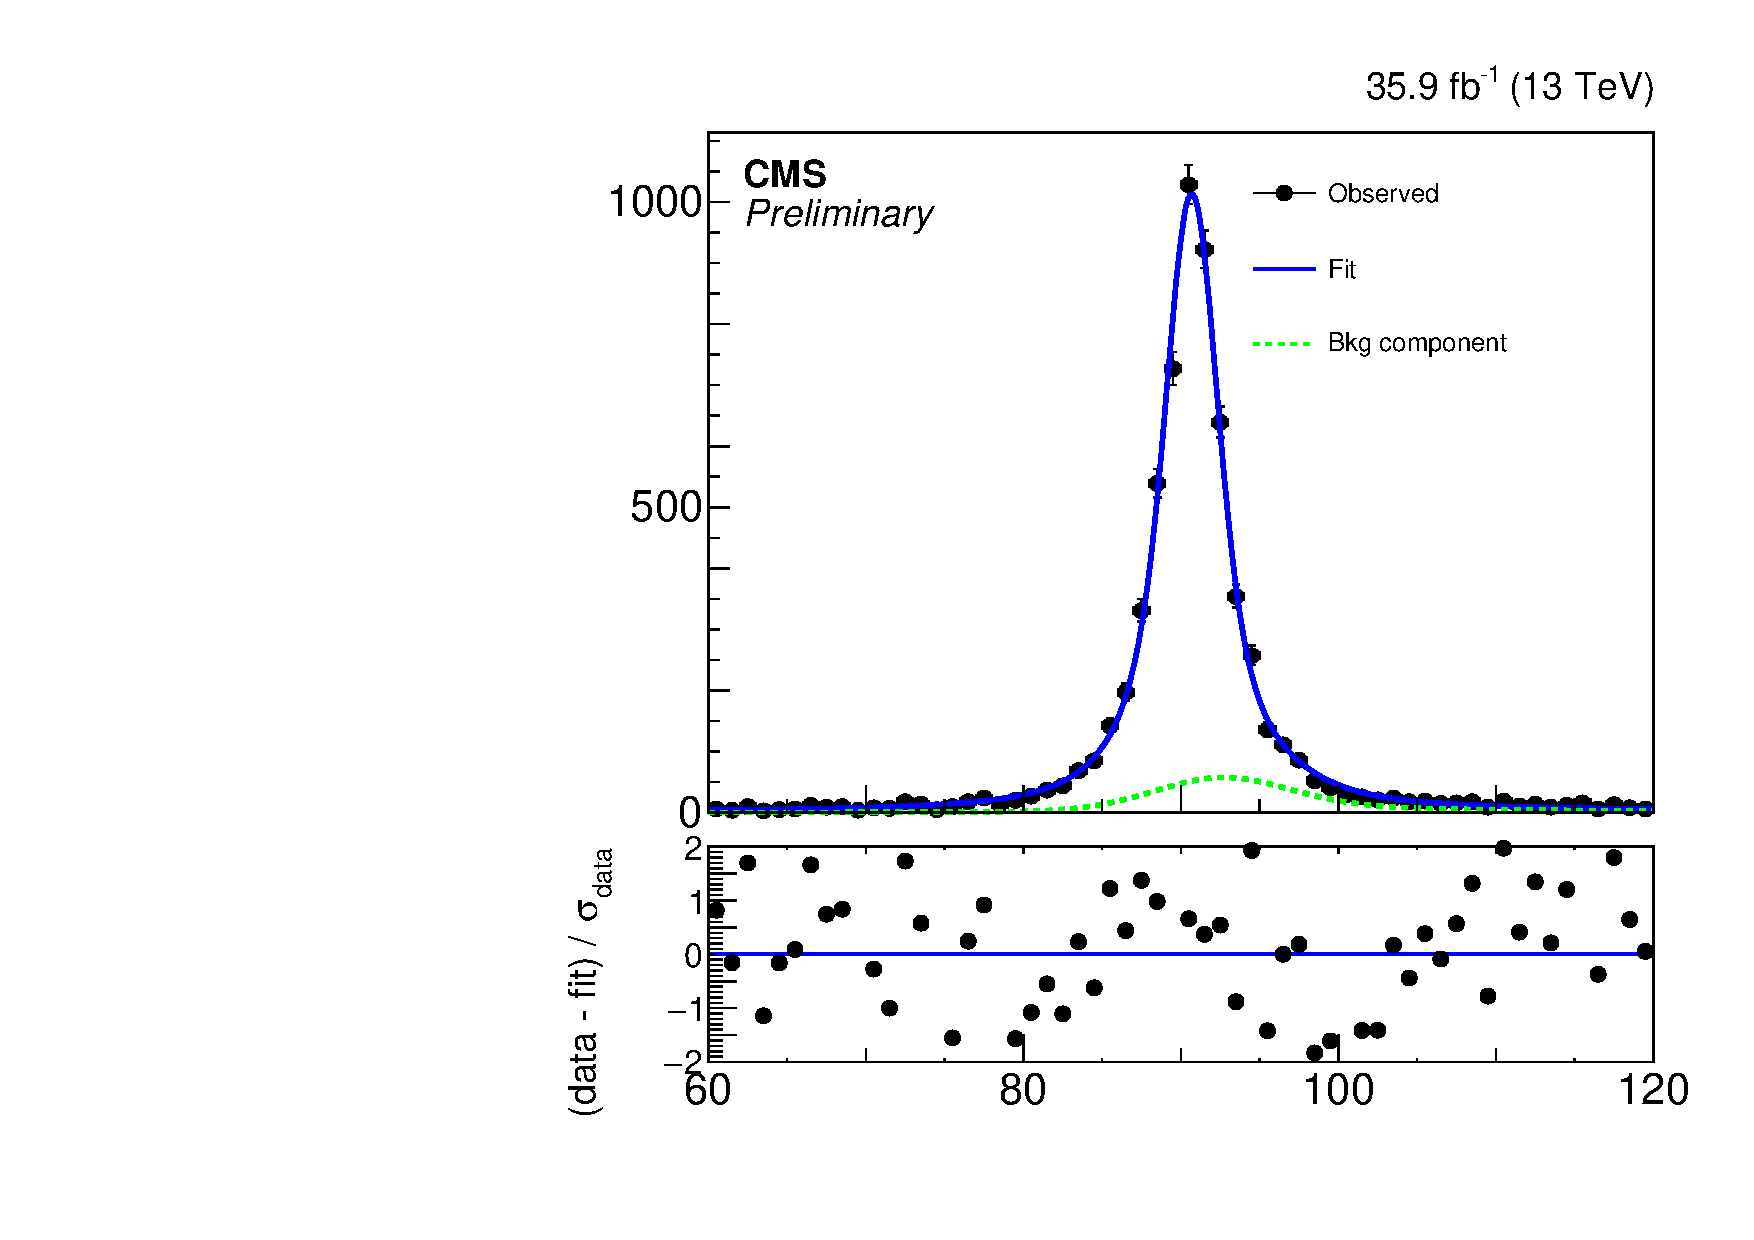
\includegraphics[width=0.48\linewidth]{Analysis/Figures/fit_data_ee_pt_200_250.pdf}
    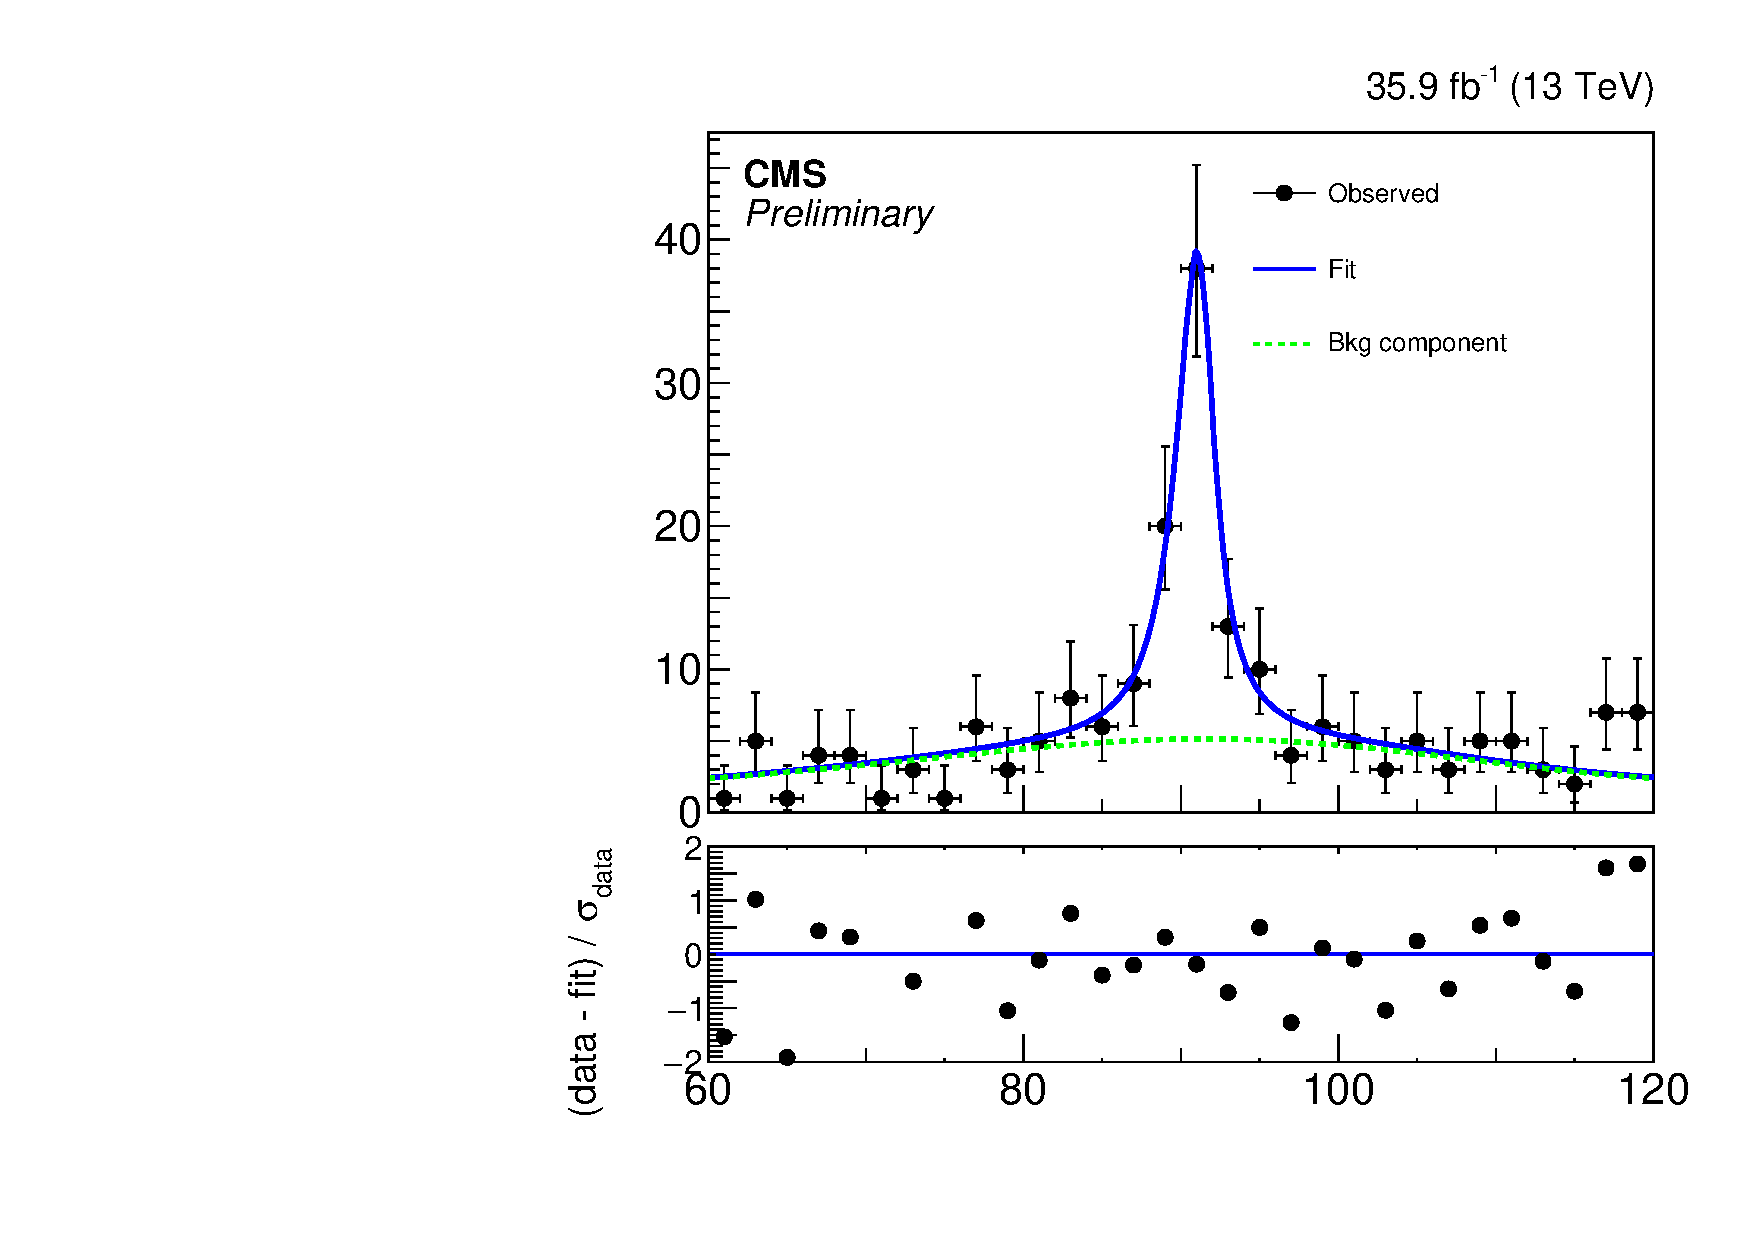
\includegraphics[width=0.48\linewidth]{Analysis/Figures/fit_data_eg_pt_200_250.pdf}
    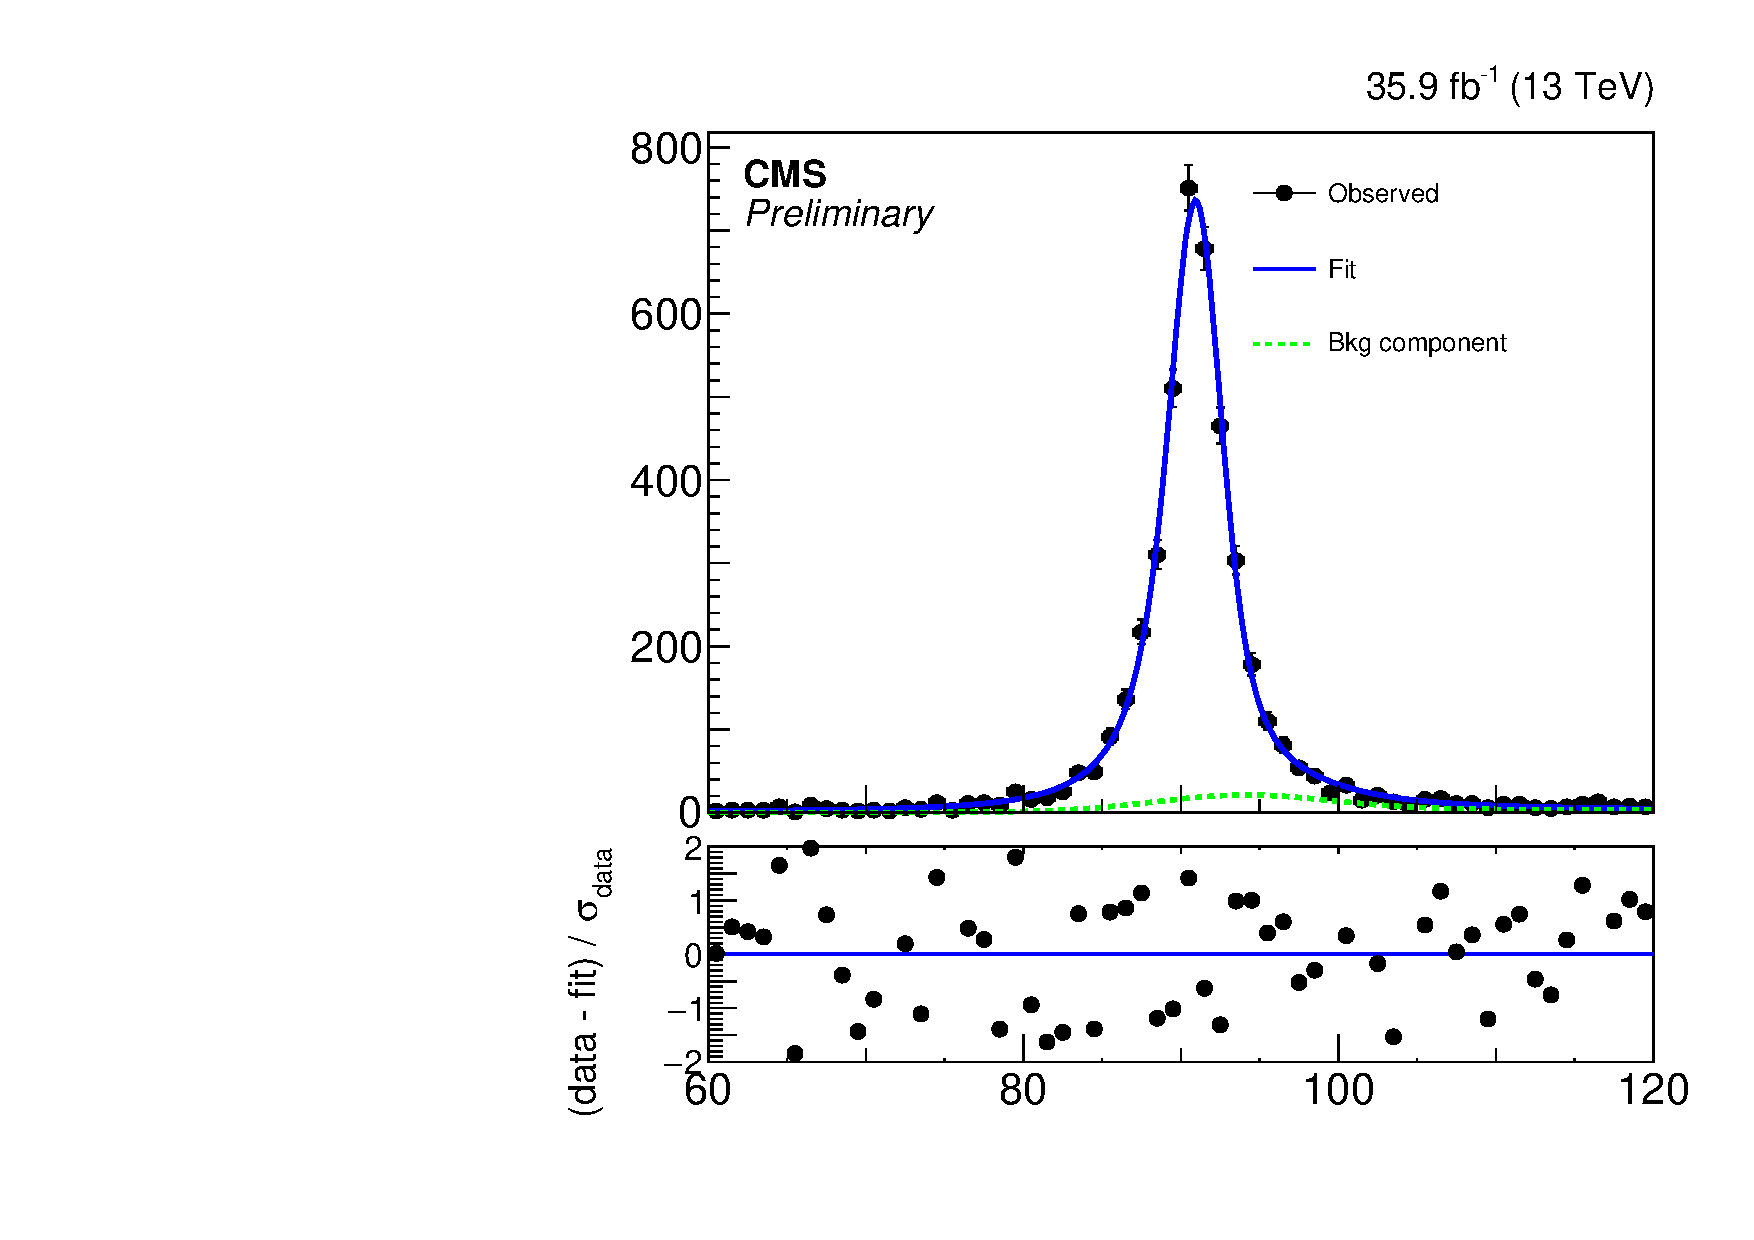
\includegraphics[width=0.48\linewidth]{Analysis/Figures/fit_data_ee_pt_250_6500.pdf}
    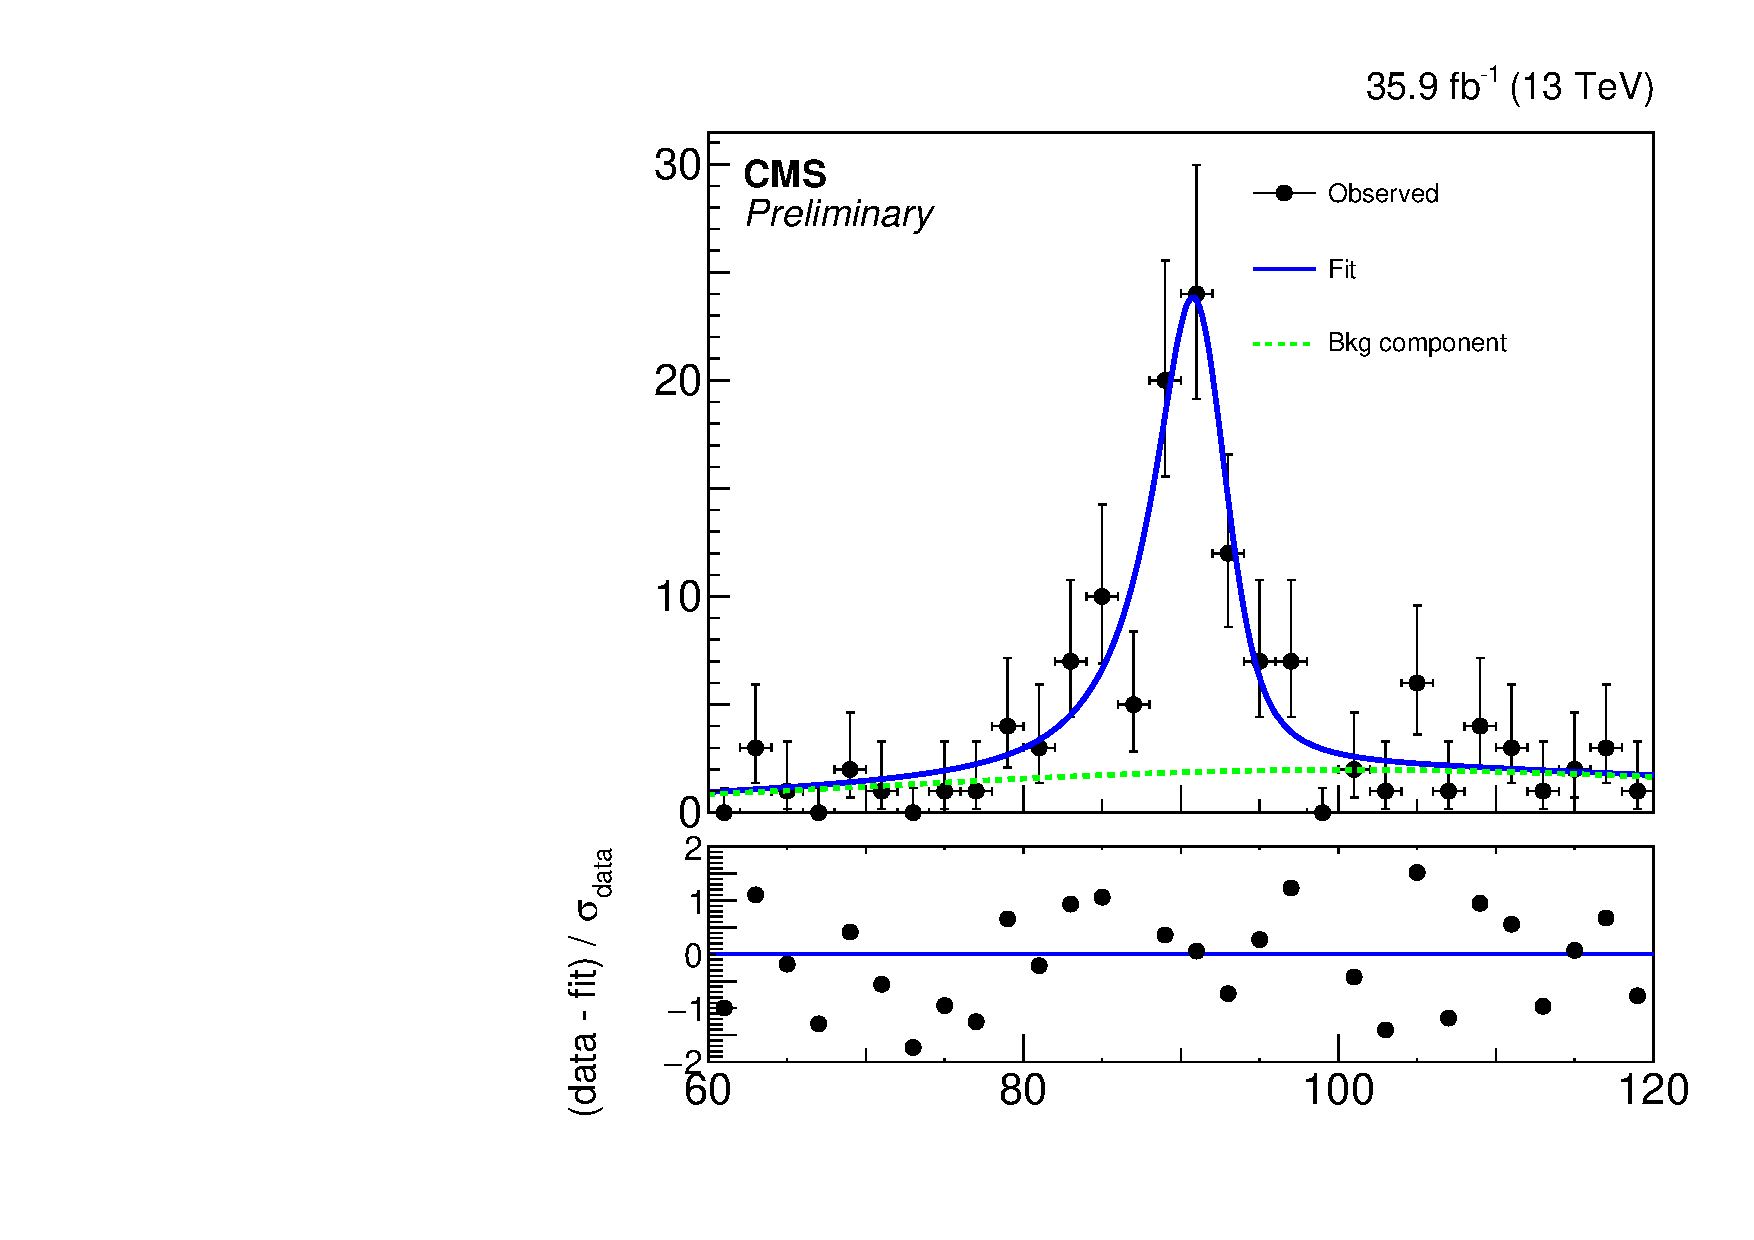
\includegraphics[width=0.48\linewidth]{Analysis/Figures/fit_data_eg_pt_250_6500.pdf}
    \caption{
      Fits to the mass distributions for \Pe\Pe\ (left) and \Pe\Pgg\ (right) selections, in bins of probe $\pt$: $175 < \pt < 200\GeV$ (top), $200 < \pt < 250\GeV$ (middle), $\pt > 250\GeV$ (bottom). 
      The blue solid line represents the full fit model, and the green dashed line its background component.
    }
    \label{fig:efake_fits}
  \end{center}
\end{figure}

The proxy sample for the background estimation is obtained by identical event selection as that described in Sec.~\ref{sec:event_selection}, but with the pixel-seed veto inverted on the photon candidate object.

%%% Systematic uncertainties in this method to estimate the electron misidentification background can be categorized to those related to the TP fit (described in Section~\ref{subsec:idsf}) and those related to the applicability of the $R_{\Pe}$ factor.

Figure~\ref{fig:efake_frate} shows the derived $R_{\Pe}$ factor as a function of \ETg. 
The electron proxy sample is reweighted by $R_{\Pe}$ depending on the \pt\ of the electron object.

%%% this file has charged PF veto included, need to swap out
\begin{figure}[htbp]
  \begin{center}
    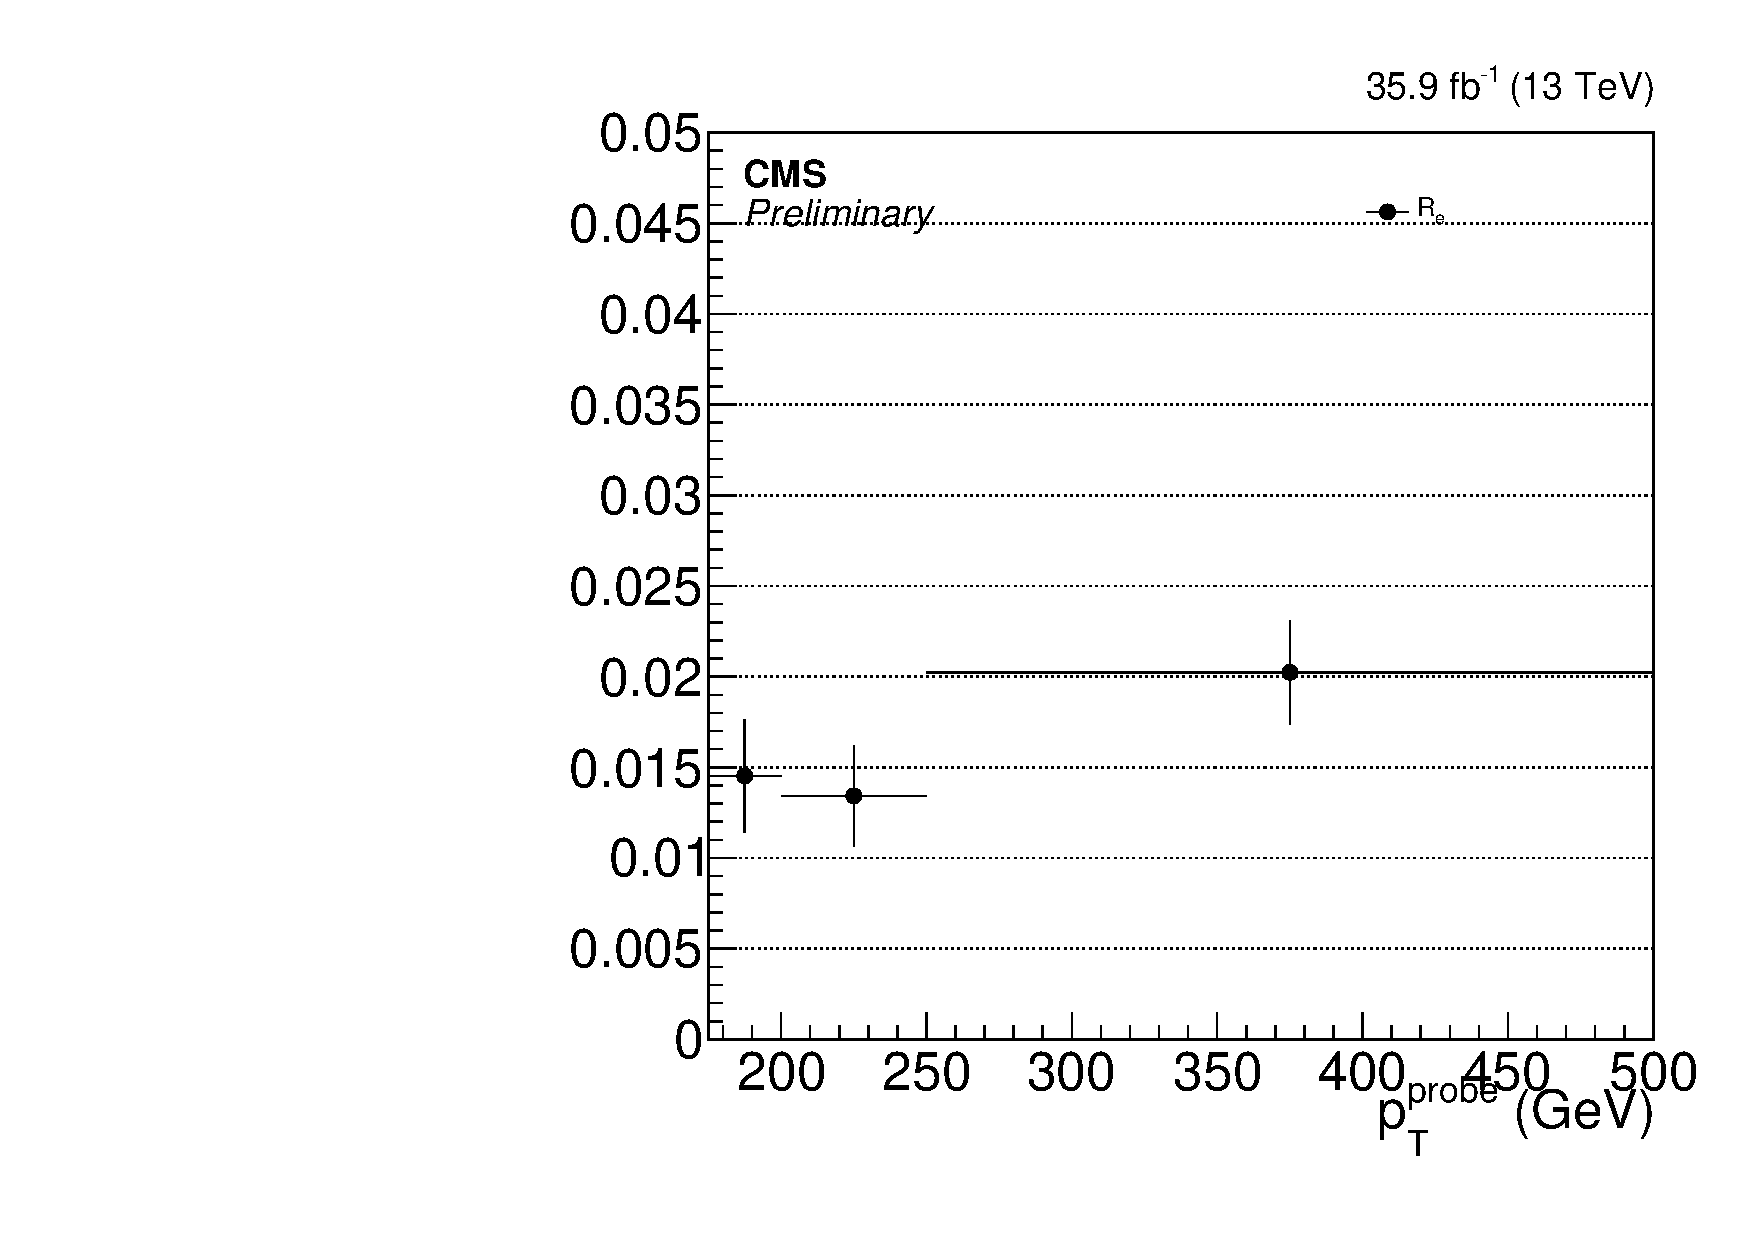
\includegraphics[width=0.48\linewidth]{Analysis/Figures/frate_data_ptalt.pdf} 
    \caption{
      Electron to photon fake rate $R_{\Pe}$.
    }
    \label{fig:efake_frate}
  \end{center}
\end{figure}

\section{Misidentified hadrons}
\label{sec:hfake}

The estimation of hadron misidentification background proceeds in multiple steps. 
First, the fraction of hadronic objects within a pool of photon candidate objects in the photon plus jet control region is measured. 
This measurement is described in detail in Section~\ref{subsec:pvsf}.
Figure~\ref{fig:impurity-compsb} and Table~\ref{tab:hfake-impurity-systs} show the final impurity and associated uncertainties as a function of \pt. 

\begin{table}[htbp]
  \centering
  \begin{tabular}{ |c|c|c c c c| }
% \hline
% \multicolumn{6}{ |c| }{Impurity (\%) for barrel medium-pixel-monoph photons in data} \\
\hline
\pt & Nominal & \multicolumn{4}{ |c| }{Sources of Systematic Uncertainty} \\
 (GeV) & & Sideband & CH Iso Shape & Signal Shape & Bgkd. Stats \\
\hline
 (175, 200)  & $4.31 \pm 0.21$ & 0.09 & 0.18 & 0.05 & 0.04 \\
 (200, 250)  & $3.39 \pm 0.17$ & 0.01 & 0.16 & 0.06 & 0.03 \\
 (250, 300)  & $2.44 \pm 0.22$ & 0.14 & 0.16 & 0.06 & 0.05 \\
 (300, 350)  & $1.99 \pm 0.23$ & 0.12 & 0.16 & 0.07 & 0.08 \\
 (350, 400)  & $1.43 \pm 0.28$ & 0.23 & 0.11 & 0.05 & 0.10 \\
 (400, $\infty$)  & $0.63 \pm 0.30$ & 0.27 & 0.09 & 0.05 & 0.05 \\
\hline
\end{tabular}

  \caption{Impurities for photons as a function of \pt.}
  \label{tab:hfake-impurity-systs}
\end{table}

\begin{figure}[htbp]
  \centering
  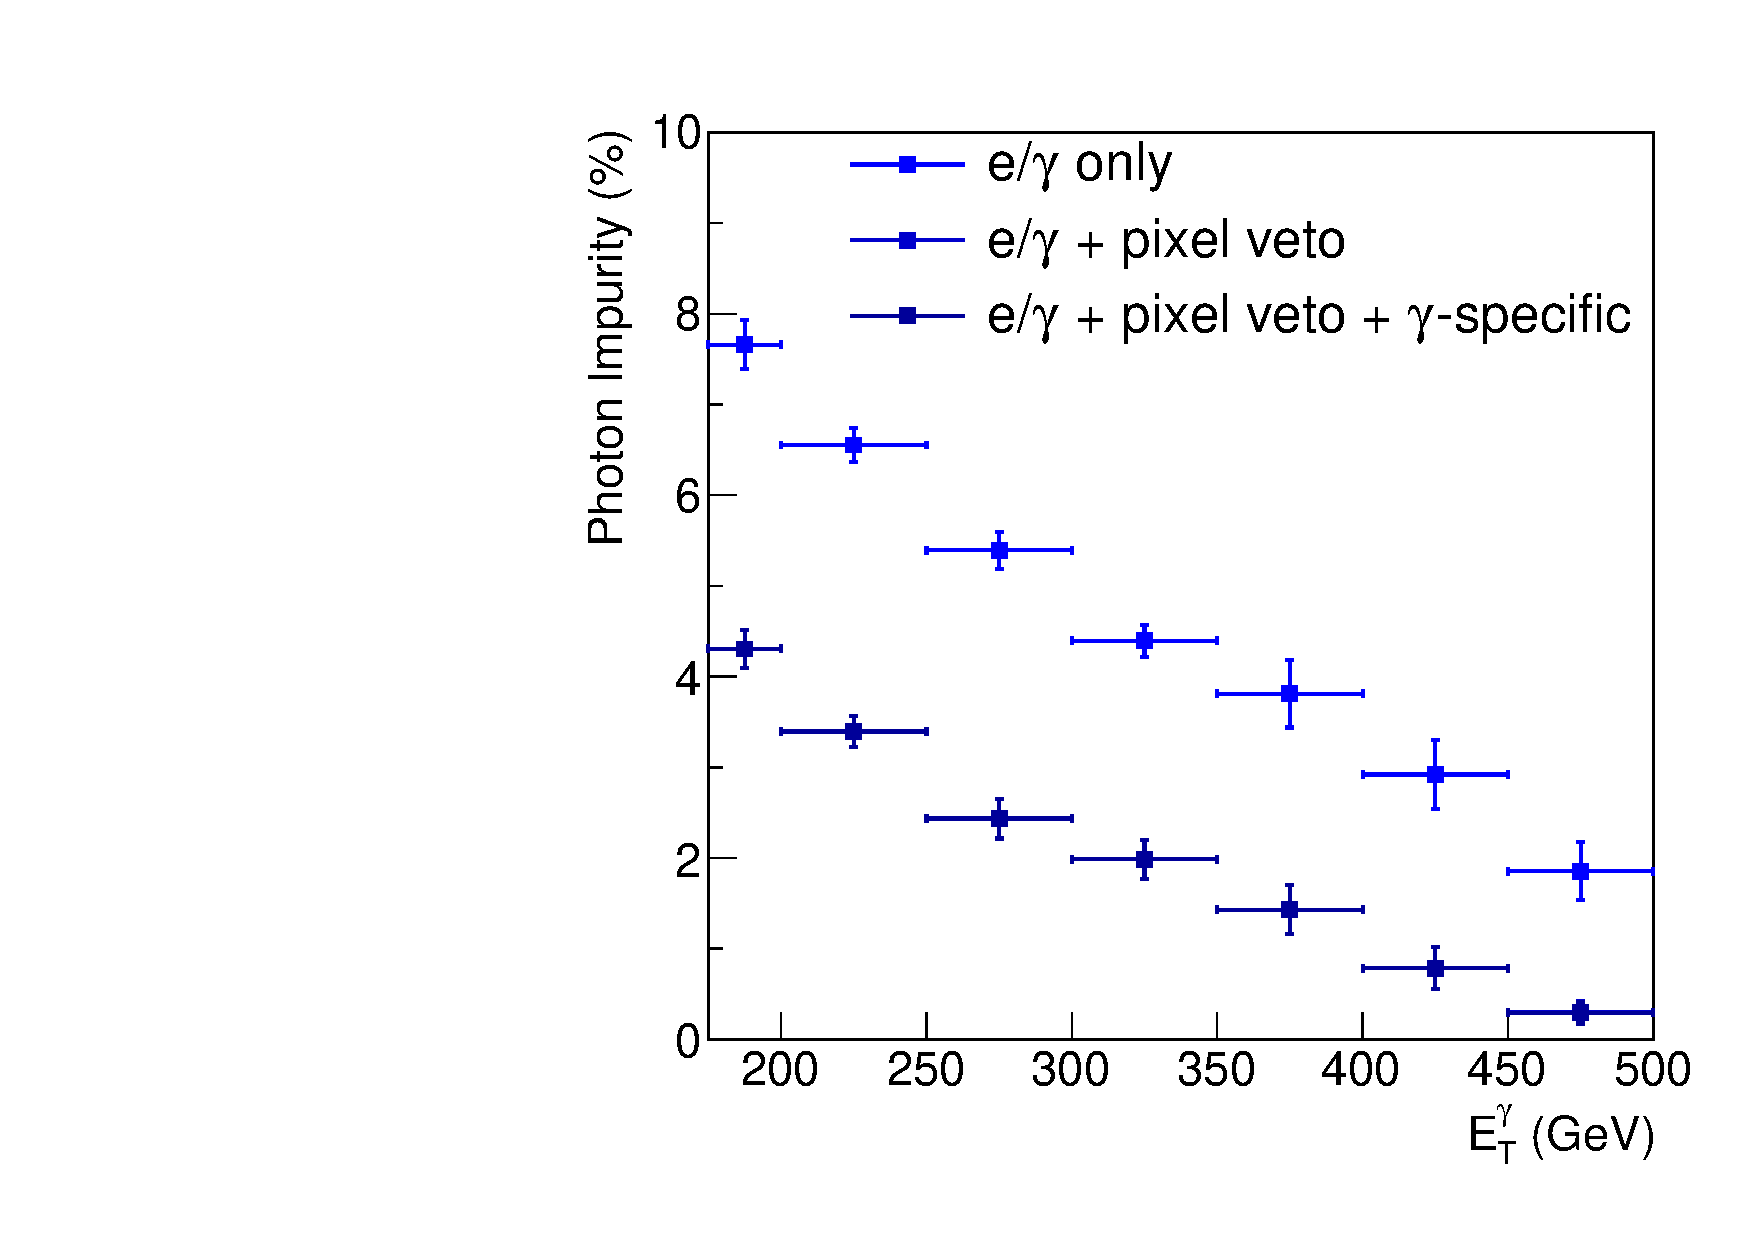
\includegraphics[width=0.45\linewidth]{Analysis/Figures/hfake/plot_impurity_barrel_medium.pdf}
    \caption{
    Impurities for photons as a function of \pt. 
    The different bands show the effects of adding different stages of the full ID, starting with the baseline ID and isolation and successively adding the pixel seed veto.
  }
  \label{fig:impurity-compsb}
\end{figure}

Following this measurement, another control sample is formed where the photon in the photon plus jet sample is replaced by a hadronic proxy object. 
The hadronic proxy object is a reconstructed photon object which pass the photon ID described in Section~\ref{sec:photons} with the execption of failing at least one of the following cuts: 
\begin{itemize}
\item $\sieie < 0.01022$
\item PF Charged Hadron isolation $< 0.441$ GeV .
\end{itemize}
Additionally, we apply a $\met < 60$ GeV cut to make this region orthogonal to the signal region of the analysis.
  
The hadronic transfer factor $R_{h}$, which measures the rate at which hadronic proxy objects result in hadrons that are misidentified as candidate photons, is obtained by dividing the estimated number of misidentified hadrons in the photon plus jet sample by the number of events in the hadron proxy + jet control region as a function of \pt. 
Figure~\ref{fig:hadronTFactor} shows the transfer factor $R_{h}$ along with the various distributions used for its derivation.

\begin{figure}[htbp]
  \begin{center}
    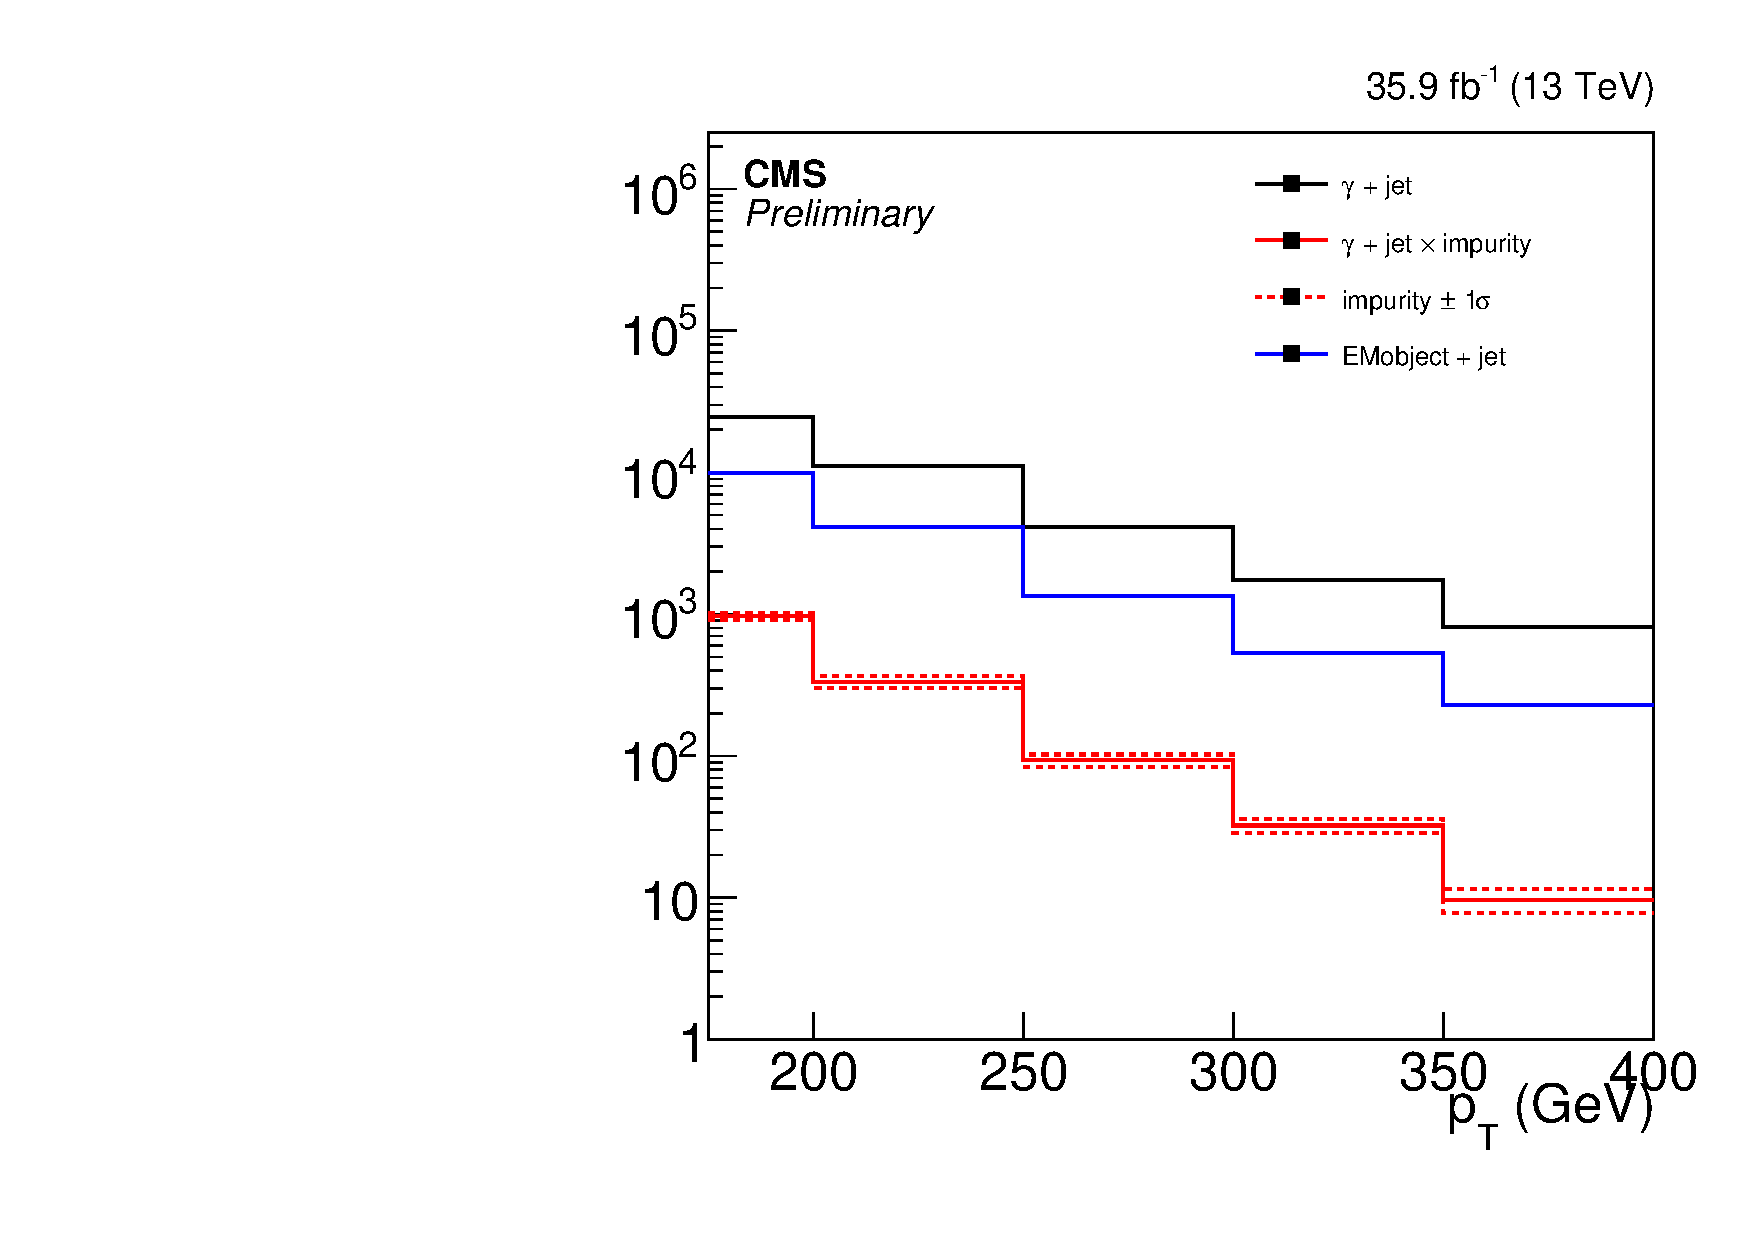
\includegraphics[width=0.45\linewidth]{Analysis/Figures/hfake/distributionsNom.pdf}
    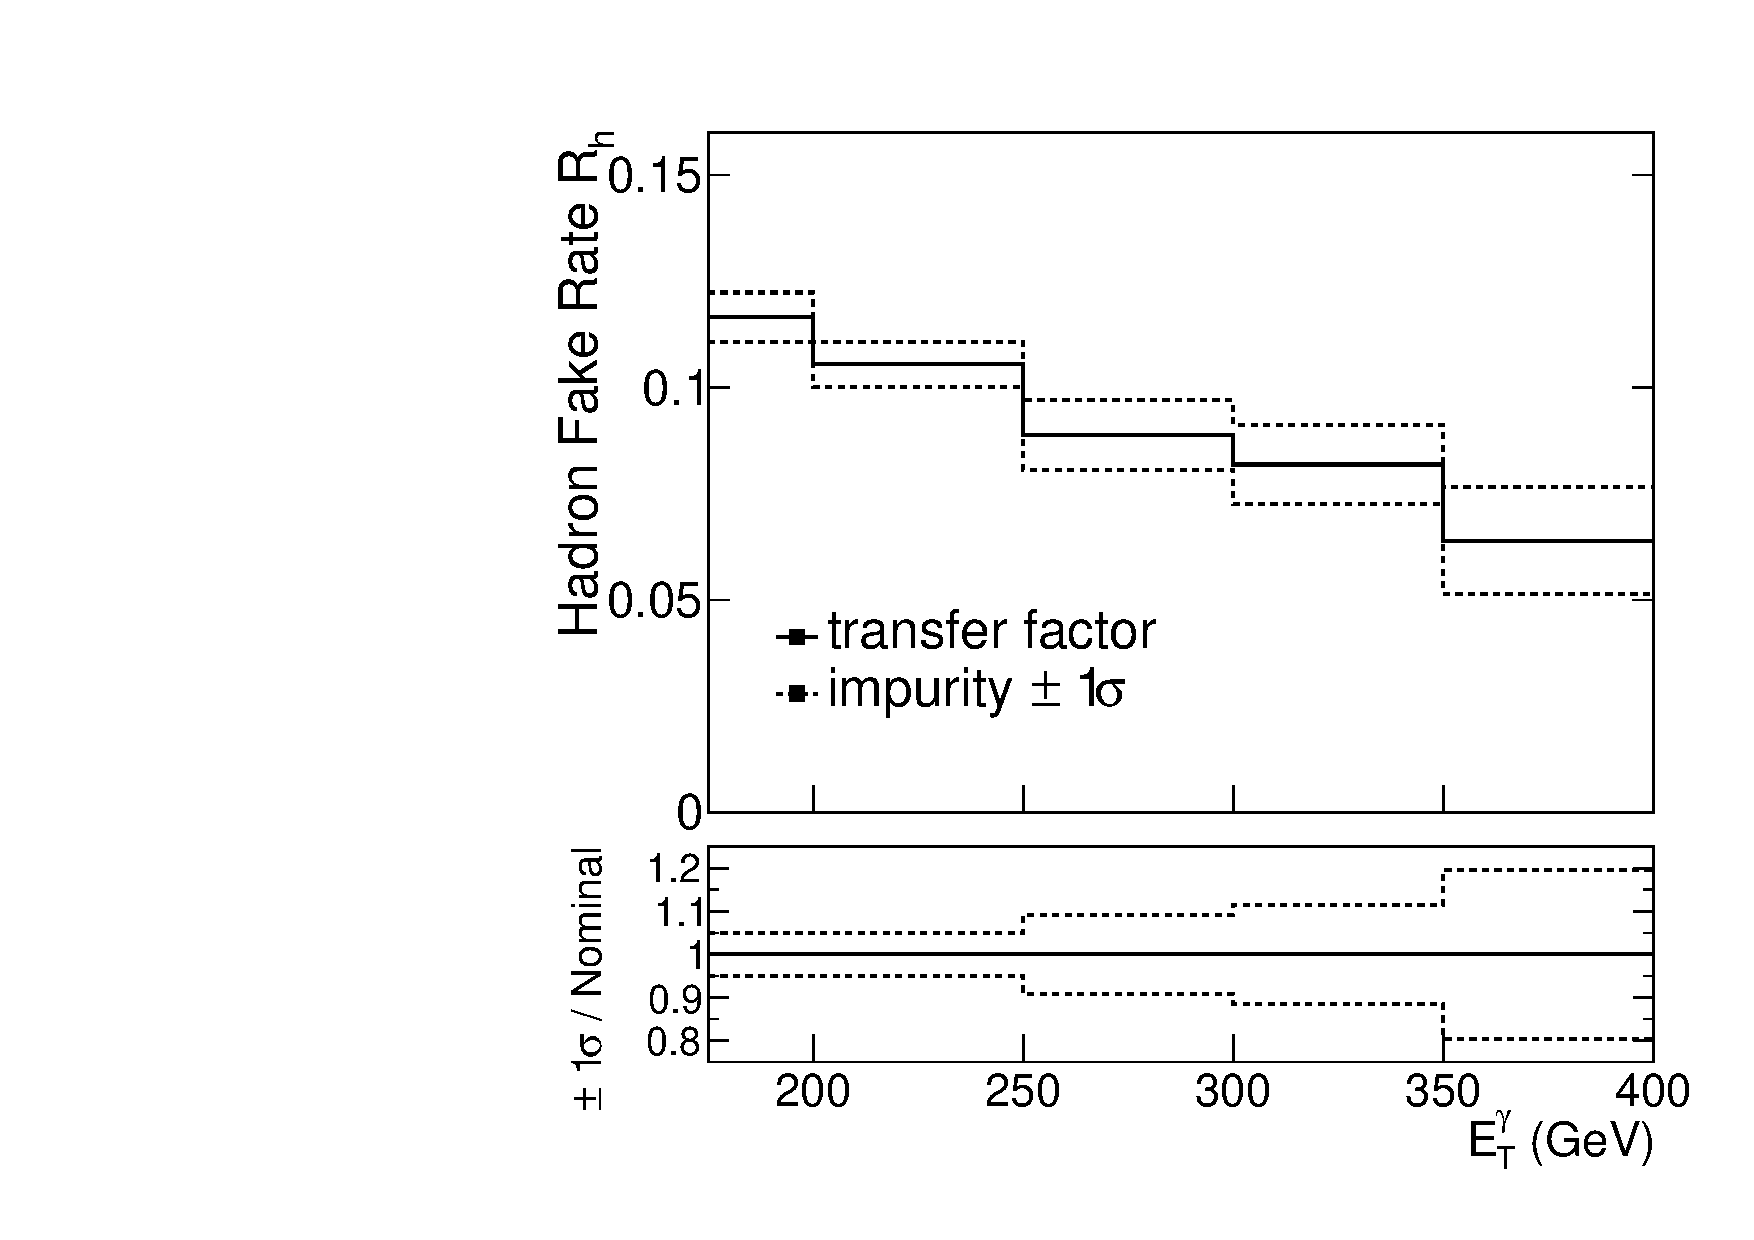
\includegraphics[width=0.45\linewidth]{Analysis/Figures/hfake/tfactorNom.pdf}
    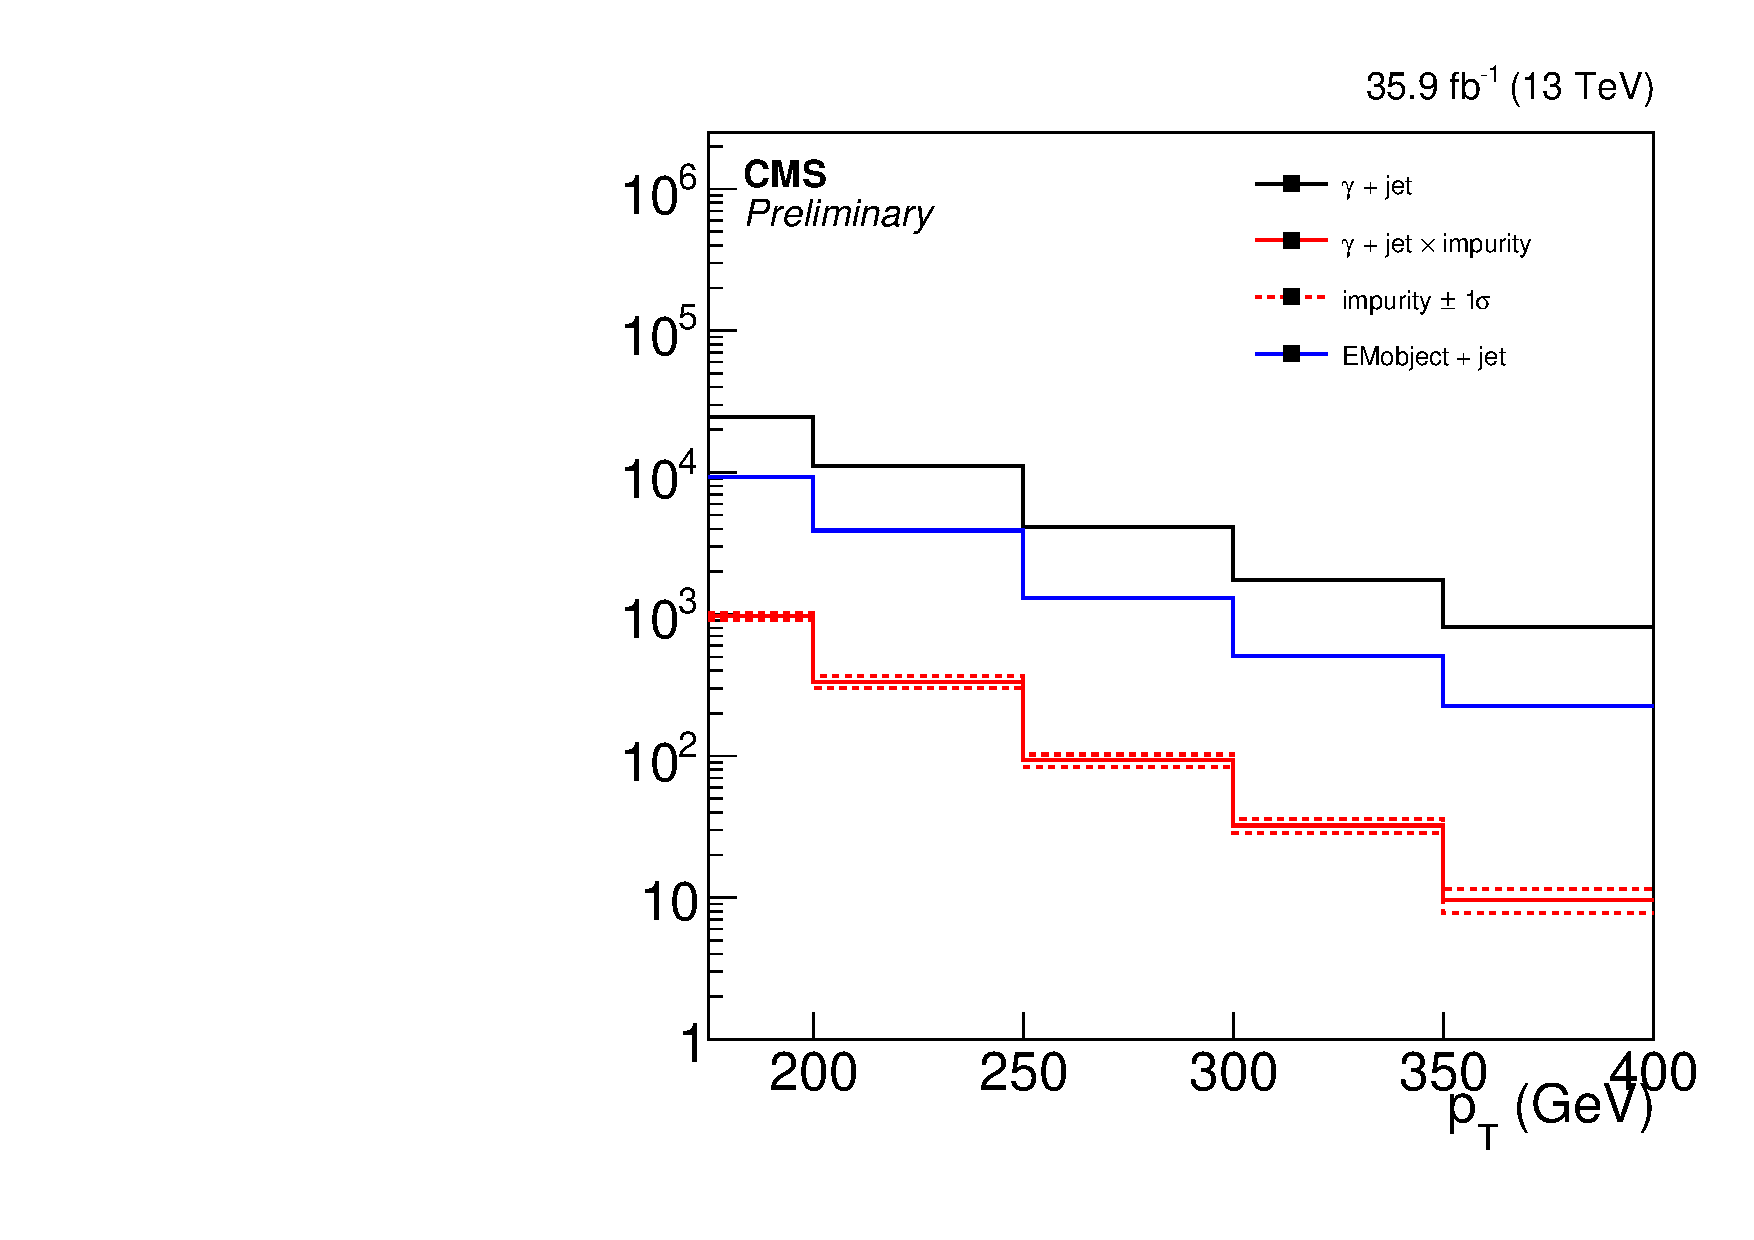
\includegraphics[width=0.45\linewidth]{Analysis/Figures/hfake/distributionsTight.pdf}
    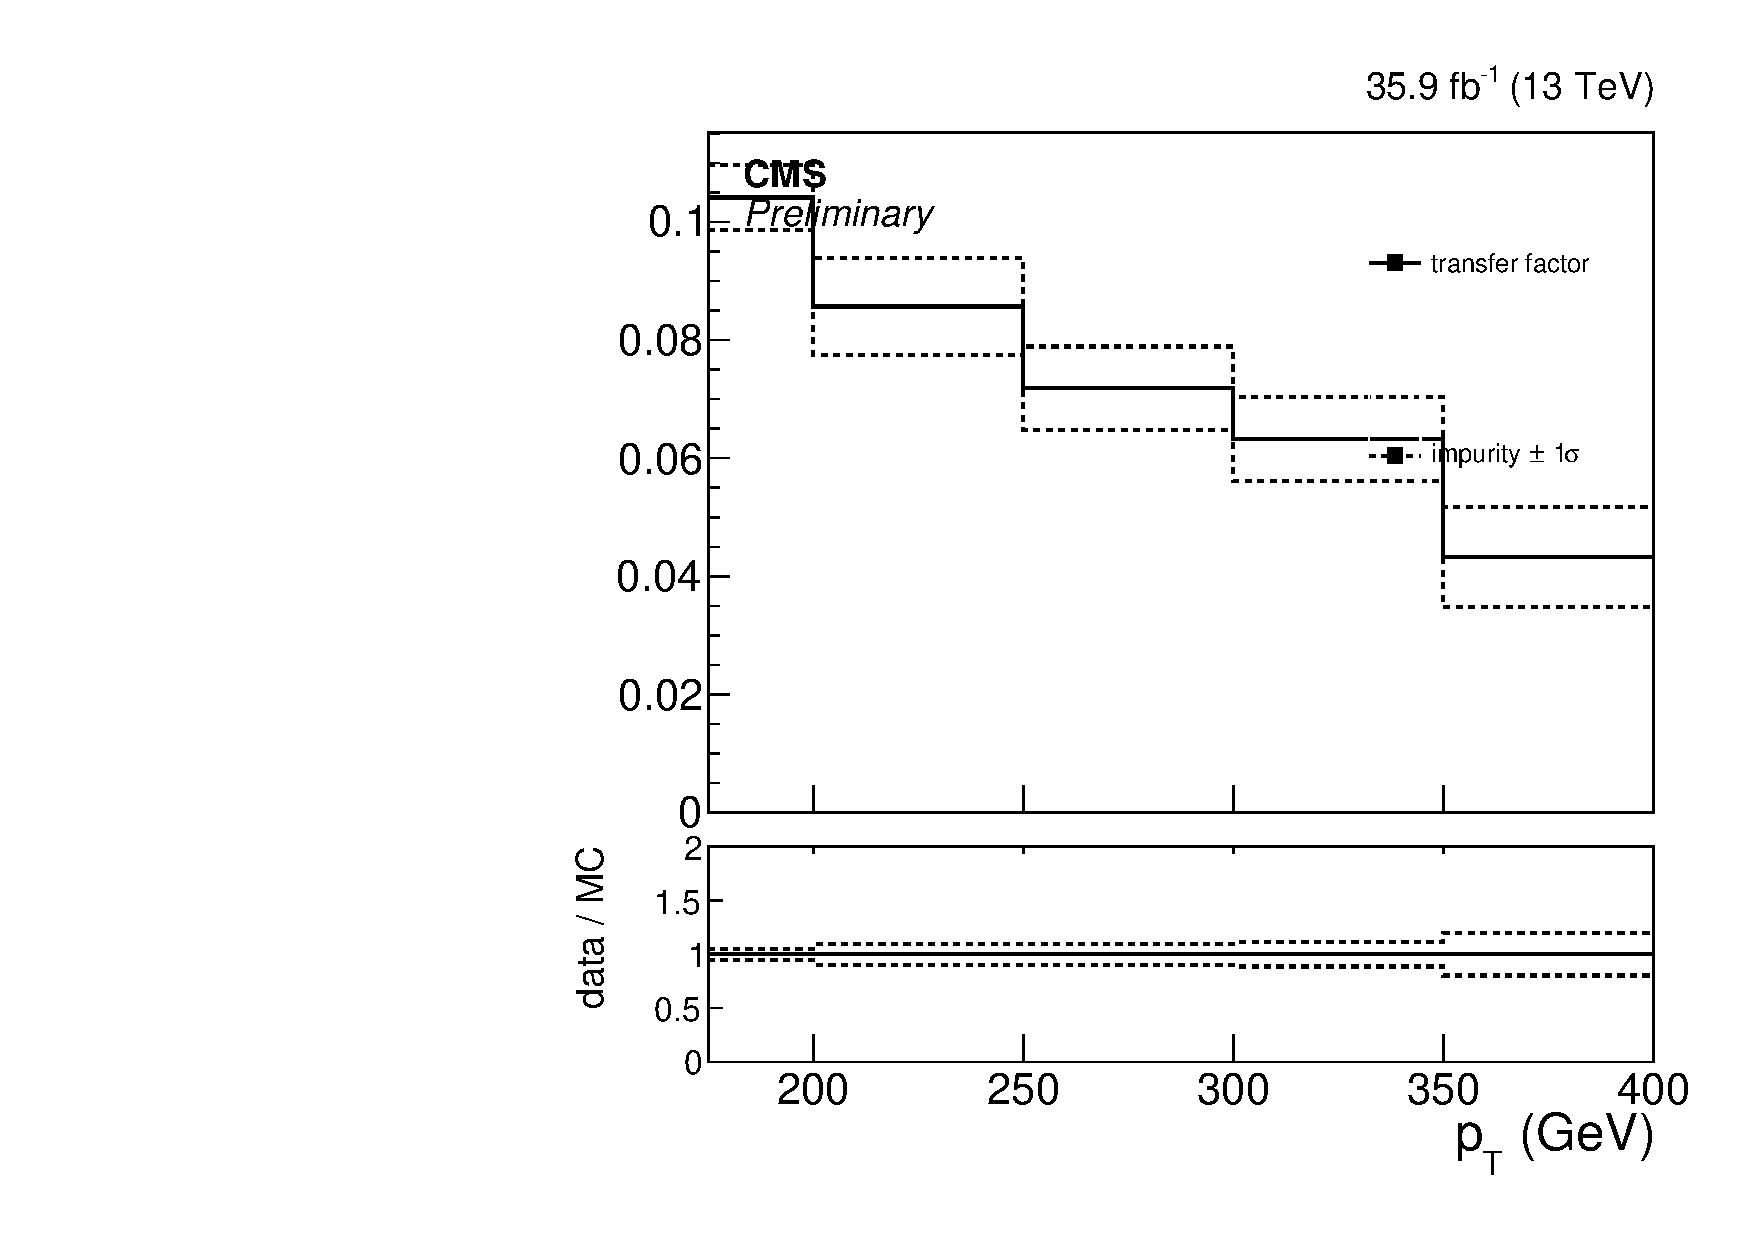
\includegraphics[width=0.45\linewidth]{Analysis/Figures/hfake/tfactorTight.pdf}
    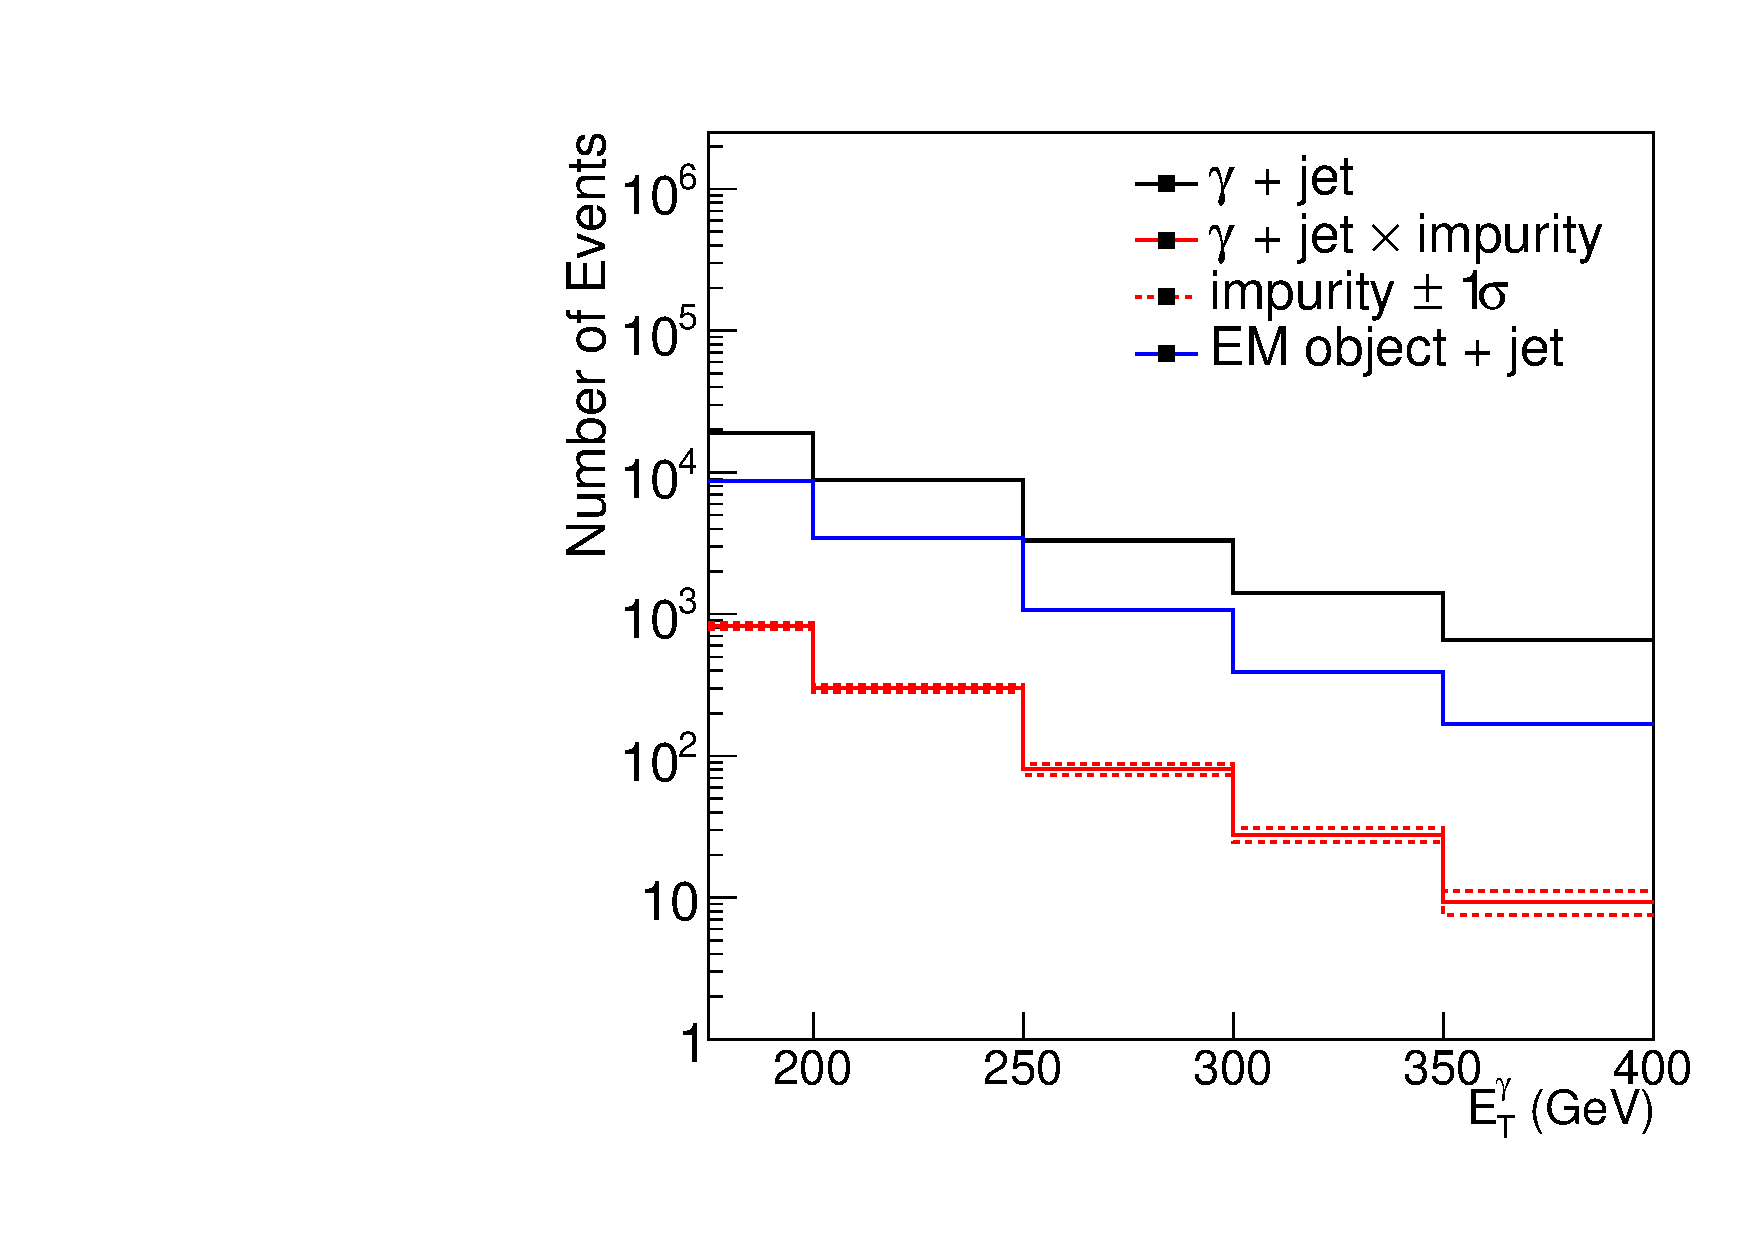
\includegraphics[width=0.45\linewidth]{Analysis/Figures/hfake/distributionsLoose.pdf}
    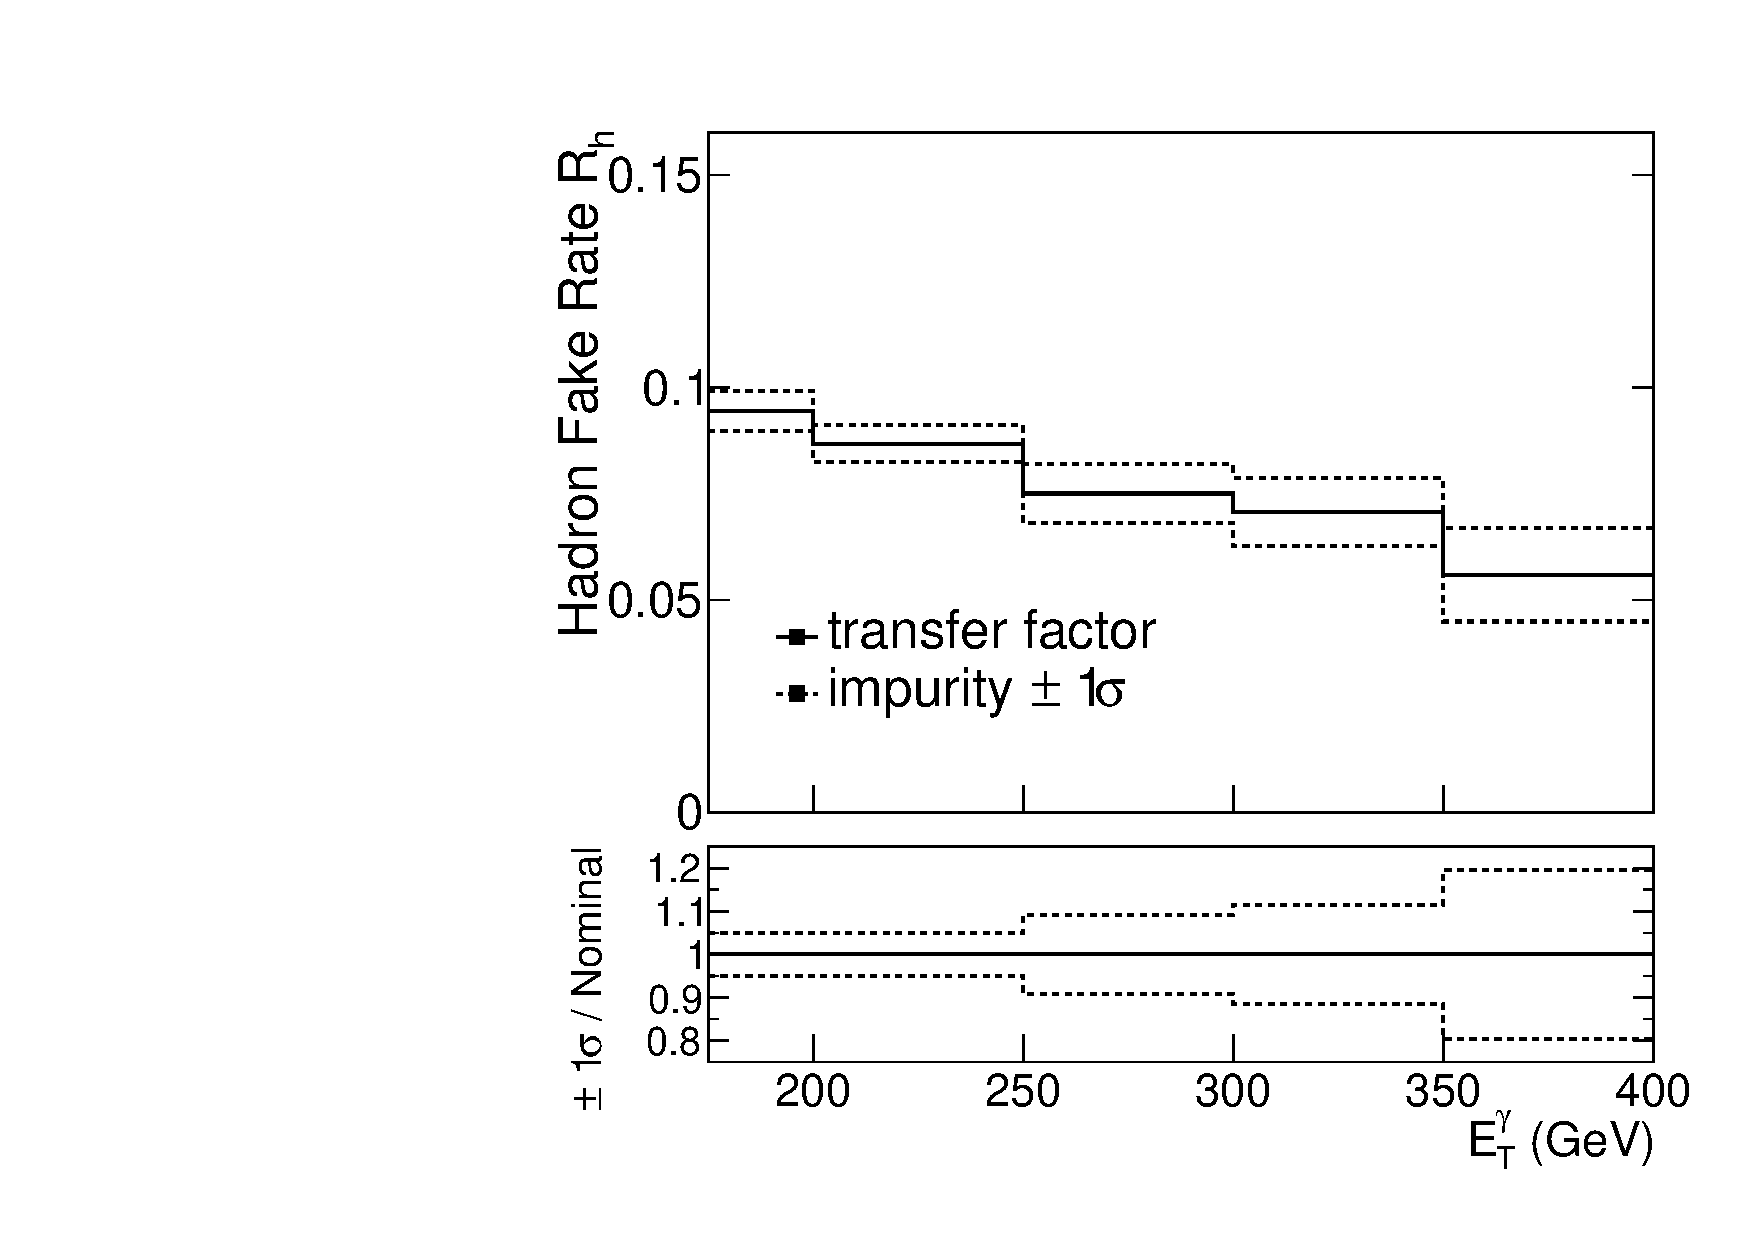
\includegraphics[width=0.45\linewidth]{Analysis/Figures/hfake/tfactorLoose.pdf}
    \caption{
      Left: The \pt\ distribution of the candidate photon object in the photon + jet control sample (black), the result of scaling it with the impurity (red), and the \pt\ distribution of the hadronic proxy object in the proxy + jet control sample (blue).
      Right: Hadronic transfer factor $R_{h}$, which is the ratio of the red and blue distributions in the left plot. 
      Top: Nominal hadron proxy object. 
      Middle: Tighter hadron proxy object. 
      Bottom: Looser hadron proxy object.
    }
    \label{fig:hadronTFactor}
  \end{center}
\end{figure}

Finally, a third control sample of events with a hadronic proxy object and $\met > 170$ GeV is prepared. 
Under the assumption that the $R_{h}$ stays constant regardless of whether the event has a high-\pt\ jet or \met, this proxy plus \met\ sample is then weighted by $R_{h}$ to arrive at an estimate of the misidentified hadron plus \met\ background of this analysis.

%%% need to update these numbers
To estimate the uncertainty on this background, we repeat the above method using tighter and looser definitions of the hadron proxy object.
The tighter definition differs from the nominal by the following cuts:
\begin{itemize}
\item $\rho$-corrected PF Neutral Hadron isolation $< 0.264 + 0.014 \times \pt^\gamma + 0.000019 \times \left( \pt^\gamma \right)^2$. 
\item $\rho$-corrected PF Photon isolation $< 2.362 + 0.0053 \times \pt^\gamma$,
\end{itemize}
and the looser definition differs from the nominal by the following cuts:
\begin{itemize}
\item $\rho$-corrected PF Neutral Hadron isolation $< 10.910 + 0.014 \times \pt^\gamma + 0.000019 \times \left( \pt^\gamma \right)^2$. 
\item $\rho$-corrected PF Photon isolation $< 3.630 + 0.0053 \times \pt^\gamma$.
\end{itemize}

The different distributions from the nominal, tight, and loose selections are shown in Figure~\ref{fig:hadronFakeShapes}. 
The tight and loose shapes are taken as the one sigma band around the nominal estimate. 
Additionally, there is an uncertainty coming from the estimation of the photon purity. 
Figure~\ref{fig:hadronFakePurity} shows the resulting shapes from moving the shapes generated by a one sigma shift in the purity.

\begin{figure}[htbp]
  \begin{center}
    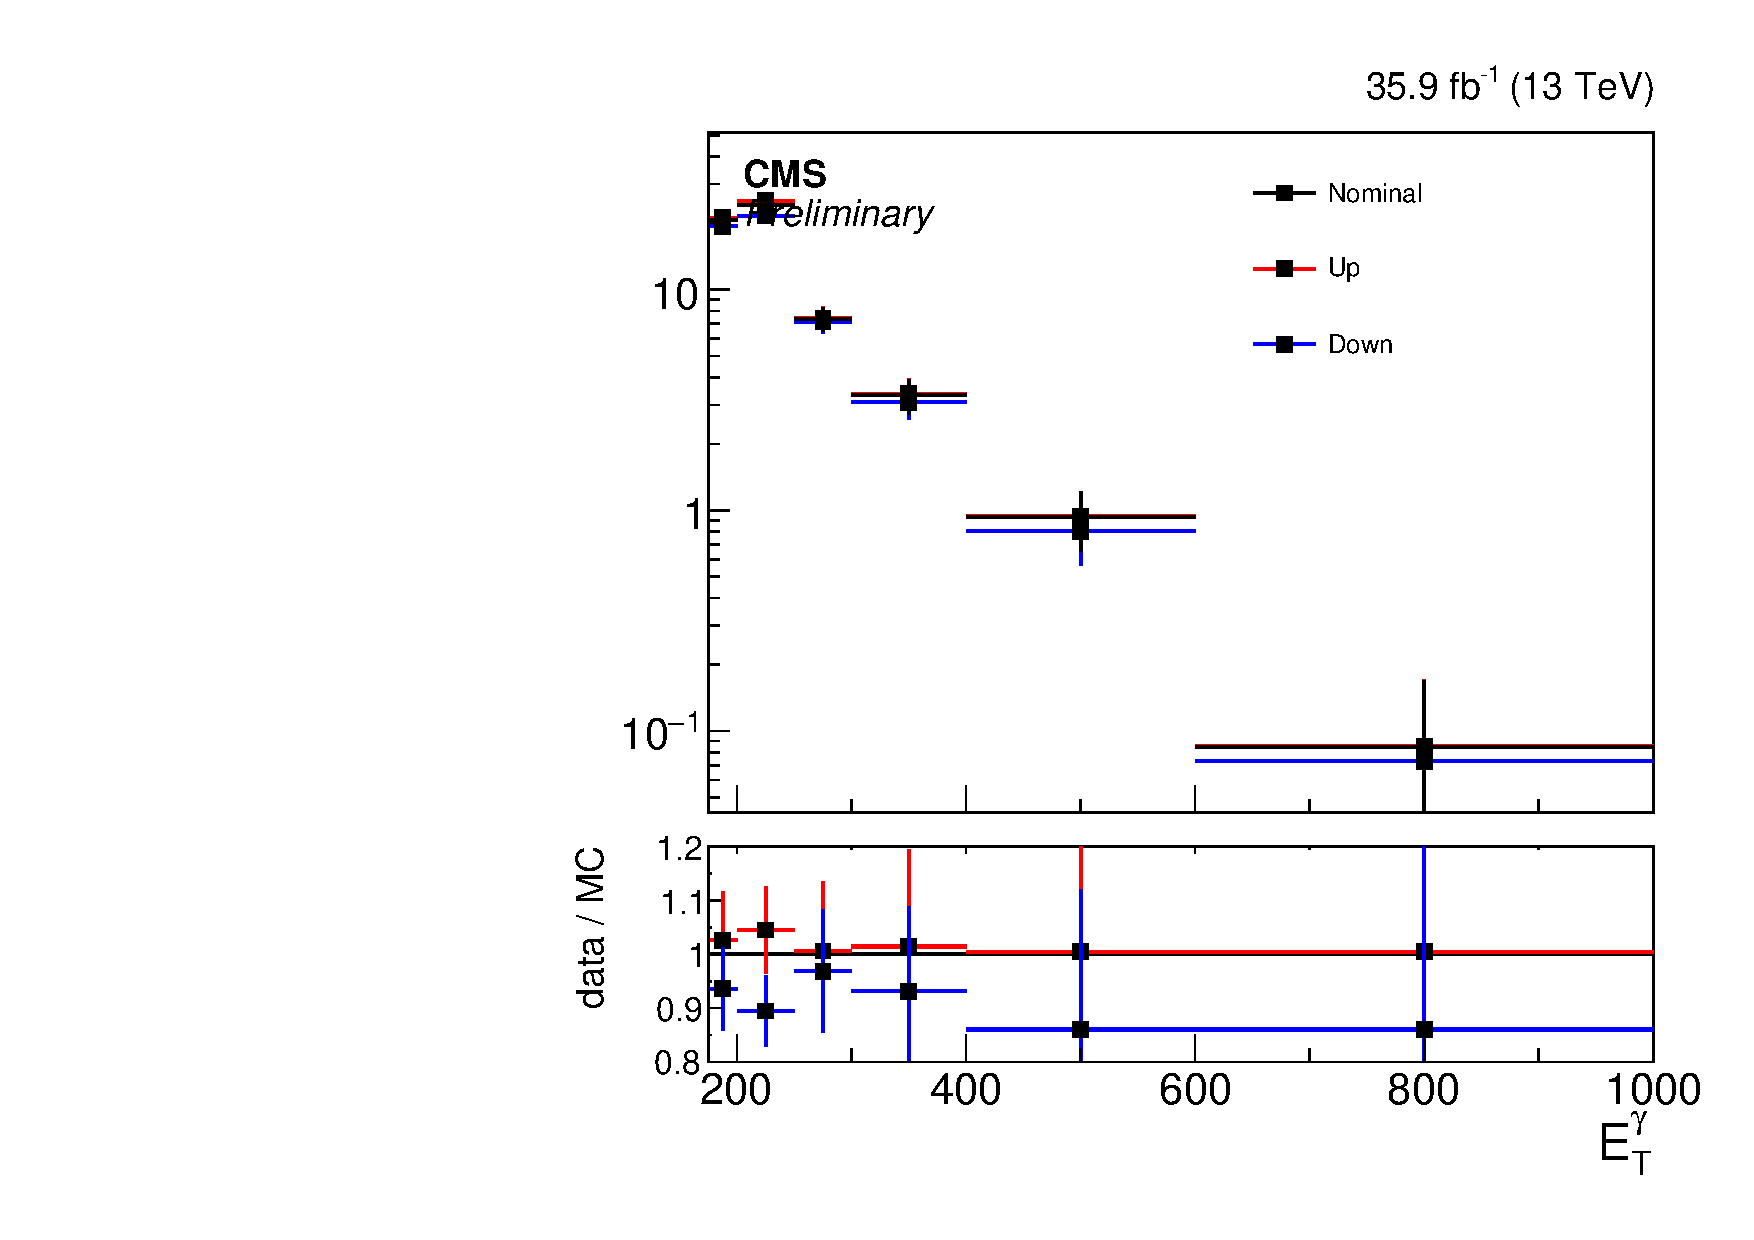
\includegraphics[width=0.48\linewidth]{Analysis/Figures/hfake/shape_sample.pdf}
    \caption{
      The \pt\ distribution of the estimated contribution from hadronic fakes in the signal region. 
      The distribution labeled Up (Down) comes from the tighter (looser) selection. 
      The systematic uncertainty resulting from this variation is around 5\% at the low end of our \pt\ range and increases to 15\% after $\pt > 400$ GeV.
    }
    \label{fig:hadronFakeShapes}
  \end{center}
\end{figure}

\begin{figure}[htbp]
  \begin{center}
    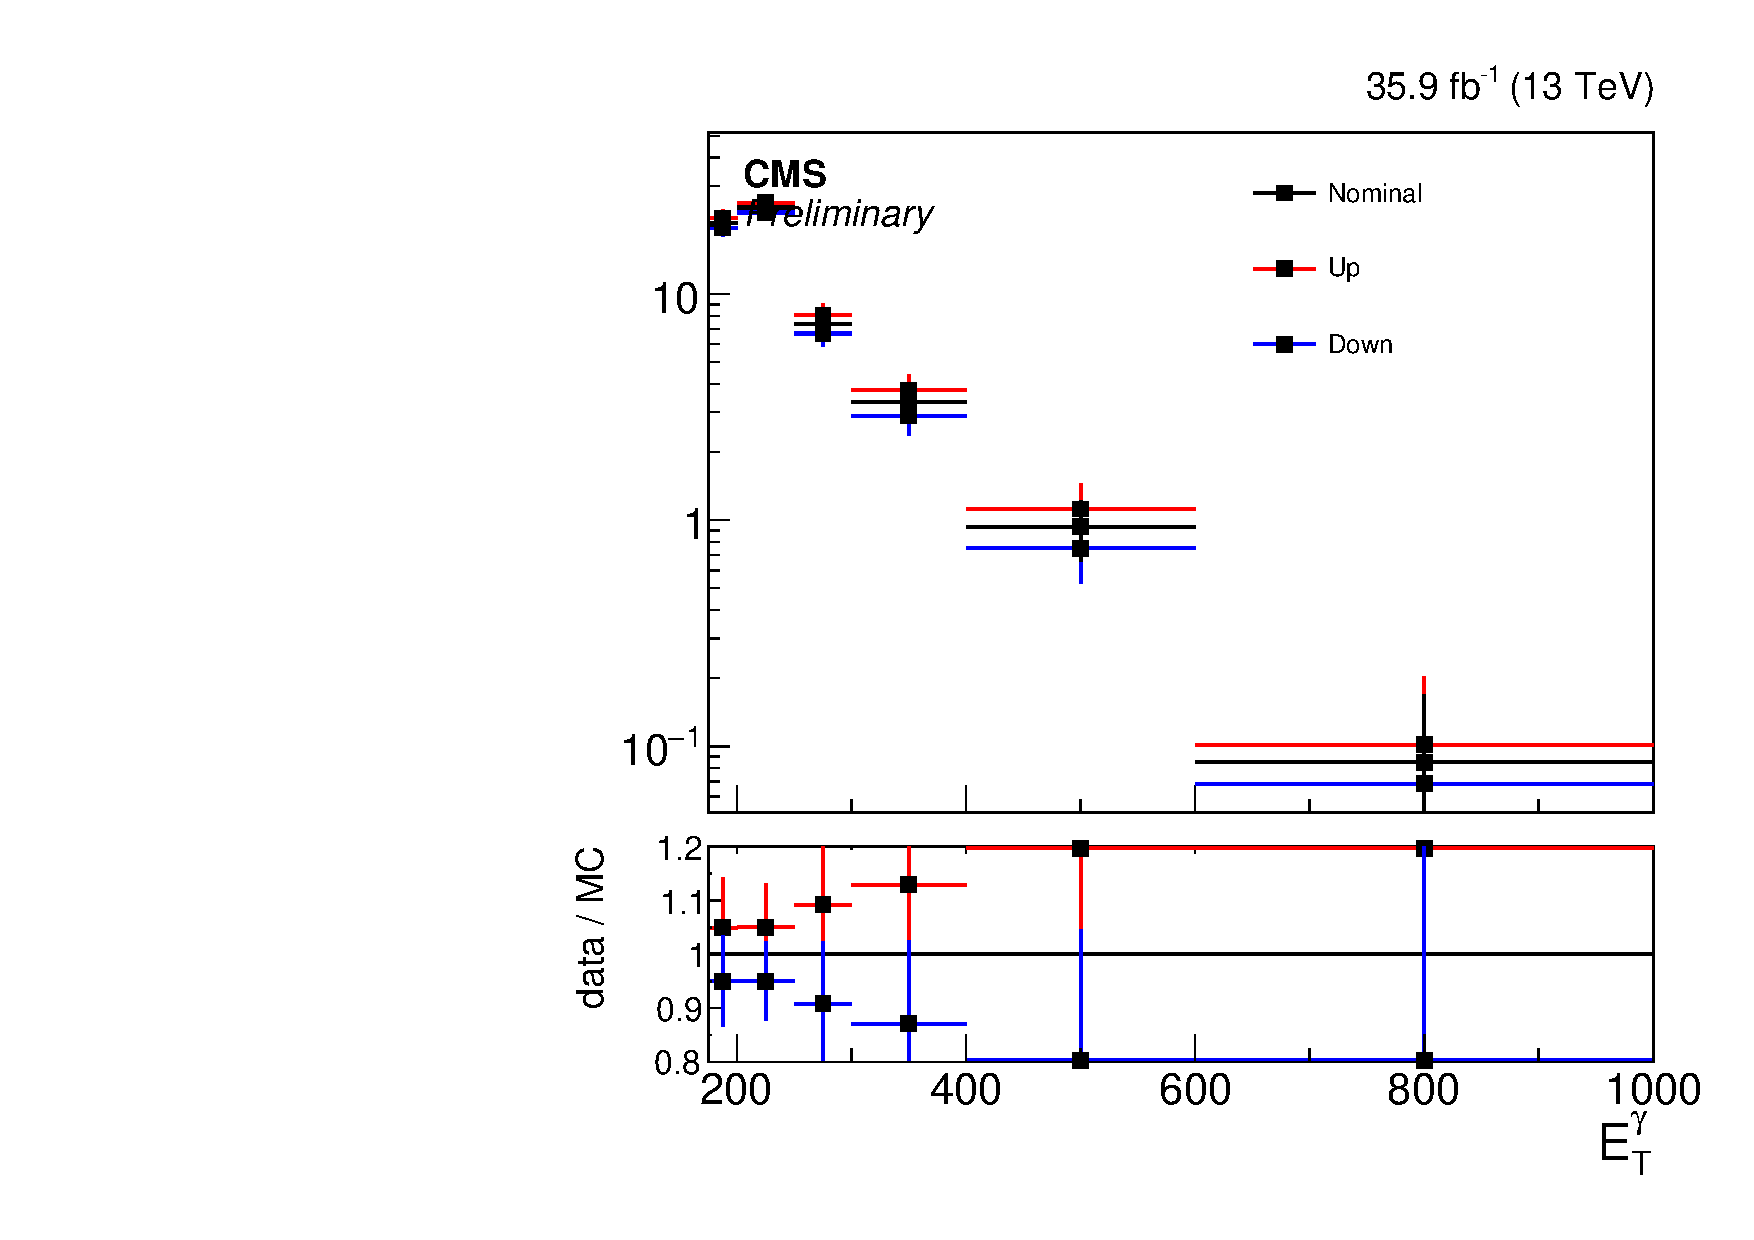
\includegraphics[width=0.48\linewidth]{Analysis/Figures/hfake/shape_purity.pdf}
    \caption{
      The \pt\ distribution of the estimated contribution from hadronic fakes in the signal region. 
      The distribution labeled Up (Down) comes from varying the purity one sigma up (down). 
      The systematic uncertainty resulting from this variation is around 5\% at the low end of the \pt\ range and increases to 20\% after $\pt > 400$ GeV.
    }
    \label{fig:hadronFakePurity}
  \end{center}
\end{figure}

\section{Spikes}
\label{sec:spikes}

\section{Beam halo}
\label{sec:beam_halo}

Figure~\ref{fig:halophi} shows the $\phi$ distribution of the halo showers obtained from the single photon data set, requiring $\ETg > 175\GeV$ and $\met > 170\GeV$. 
Here, halo showers are defined as photon objects that fail the MIP total energy cut in events where beam halo MET filter (one component of the ``MET filters'' mentioned in Section~\ref{sec:met}). 
The distribution is shifted and folded to make the peaking behavior clear. 
The resulting variable on the horizontal axis is named $\phi'$.

\begin{figure}[tbp]
  \begin{center}
    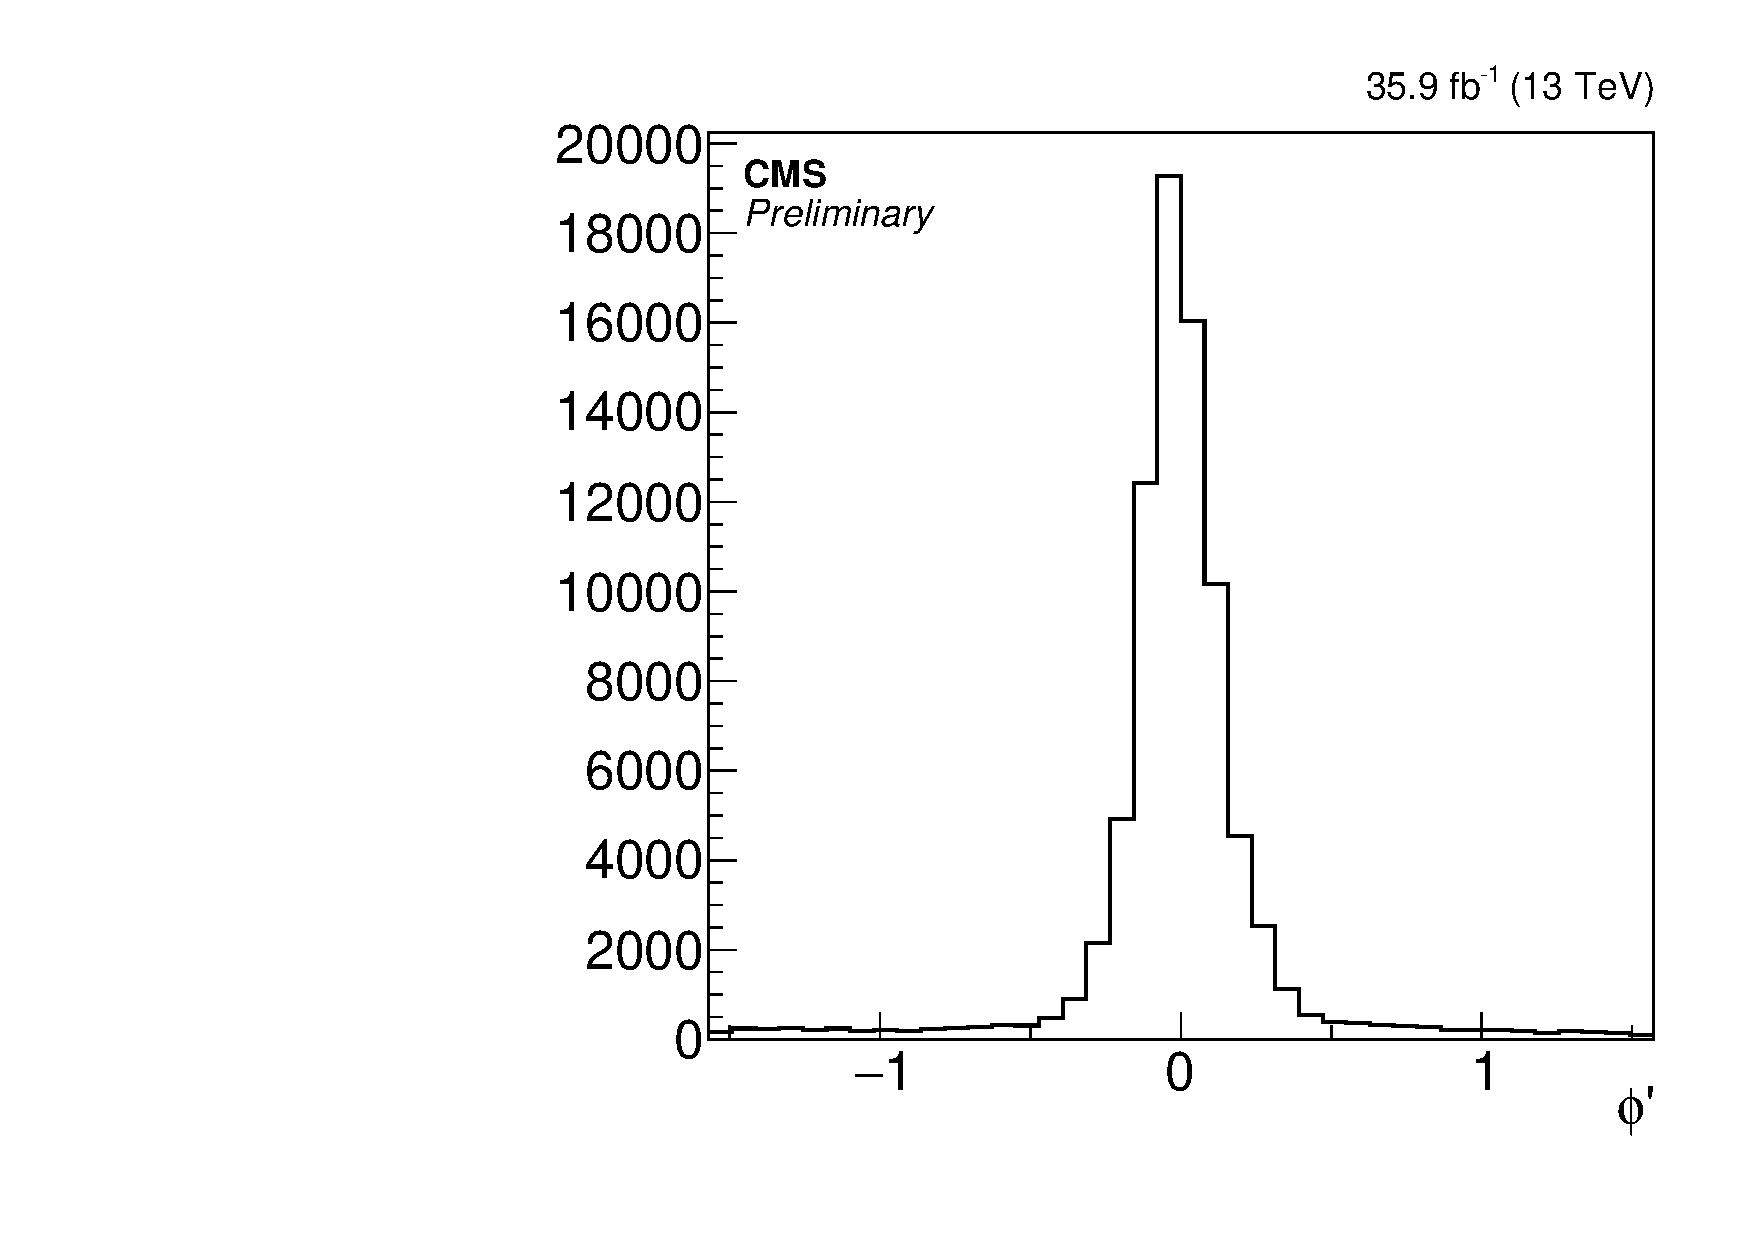
\includegraphics[width=0.45\textwidth]{Analysis/Figures/haloPhiFolded.pdf}
    \caption{
      Folded $\phi'$ distribution of the halo sample.
    }
    \label{fig:halophi}
  \end{center}
\end{figure}

The splitting of the signal region can be thought of as a two-bin fit. 
Collision processes occupy the relative fractions of phase space in the horizontal ($H$) and vertical ($V$) signal regions, $C_{H} = 1/\pi$ and $C_{V} = (\pi-1)/\pi$, respectively. 
The corresponding fractions for beam halo events are determined by selecting a halo-enriched sample where the halo identification is inverted. 
Thus, a fit of the two signal regions provides an estimate of the overall normalization of the beam halo background, denoted $h$. 
The \ETg\ dependence of the halo background is encoded in \nhalo[,i], the unit-normalized beam halo prediction in the $i^\mathrm{th}$ bin of the signal region $K \in \{H,V\}$.
Using the notation introduced in Section~\ref{sec:irreducible}, the total estimated background \TK\ in the two signal regions are
\begin{equation}
\begin{aligned}
  \TK[,i] & = C_{K} (\NZg[i] + \NWg[i]) + h \nhalo[,i] + C_{K} b_{K,i} \\
          & = C_{K} (1 + {\fZW[i]}^{-1}) \NZg[i] + h \nhalo[,i] + C_{K} b_{K,i},
\end{aligned}
\end{equation}
where $b_{K,i}$ is the total contribution to bin $i$ of region $K$ from electron and hadron misidentification, ECAL spikes, and other minor SM background processes.

\section{Other minor SM background processes}
\label{sec:minorsm}
The SM \ttg, VV\Pgg, \zllg, $\PW\to\ell\PGn$, and \gj\ processes are minor ($\sim$10\%) background processes in the signal region. 
Although \zllg\ and \gj\ do not involve high-\pt\ invisible particles, the former can exhibit large \met\ when the leptons fail to be reconstructed, and the latter when jet energy is severely mismeasured. 
The estimates for all five processes are taken from \MGvATNLO simulations at LO in QCD and can be found in Tables~\ref{tab:yield_mask_horizontal} and~\ref{tab:yield_mask_vertical}.

\section{Statistical Interpretation}
\label{sec:interpretation}

The potential signal contribution is extracted from the data via simultaneous fits to the
\ETg\ distributions in the signal and control regions defined in Section~\ref{sec:event_selection}. 
Uncertainties in various quantities are represented by nuisance parameters in the fit. 
Predictions for \zinvg, \wlng, and the beam halo backgrounds are varied in the fit. 
Beam halo is not a major background, but the extraction of its rate requires a fit to the observed distributions in the signal region.

Free parameters of the fit are the yield of \zinvg\ background in each bin of the signal regions (\NZg[i]) and the overall normalization of the beam halo background ($h$). 
Bin-by-bin yields of \wlng\ and \zllg\ samples in all regions are related to the yield of \zinvg\ through the MC prediction through the transfer factors defined in Section~\ref{sec:irreducible}. 
The transfer factors are allowed to shift within the aforementioned theoretical and experimental uncertainties.

The background-only likelihood that is maximized in the fit is
\begin{equation}
\begin{aligned}
  \mathcal{L} & = \prod_{i} \left\{ \mathcal{L_{\text{signal}}} \times \mathcal{L_{\text{single-lepton}}} \times \mathcal{L_{\text{dilepton}}} \right\} \times \mathcal{L_{\text{nuisances}}} \\
  & = \prod_{i} \left\{
    \prod_{K=H,V} \mathcal{P}\left( d_{K, i} \left| \TK[,i] (\vec{\theta} \right.) \right) \times \prod_{\ell=\Pe,\Pgm} \mathcal{P}\left( d_{\ell\Pgg, i} \left| \Tl[,i] (\vec{\theta}) \right. \right)
    \times \prod_{\ell=\Pe,\Pgm} \mathcal{P}\left( d_{\ell\ell\Pgg, i} \left| \Tll[,i] (\vec{\theta}) \right. \right)
    \right\}  \times \prod_{j} \mathcal{N}(\theta_j) \\
  & = \prod_{i} \left\{
  \begin{gathered}
    \prod\limits_{K=H,V} \mathcal{P}\biggl( d_{K, i} \biggl| \left(1 + {\fZW[,i]}^{-1}(\vec{\theta})\right) C_{K} \NZg[i] + h \nhalo[,i](\vec{\theta}) + C_{K} b_{K, i}(\vec{\theta}) \biggr. \biggr) \\
    \times \prod\limits_{\ell=\Pe,\Pgm} \mathcal{P}\biggl( d_{\ell\Pgg, i} \biggl| \frac{\NZg[i]}{\RWl[,i](\vec{\theta}) \fZW[,i] (\vec{\theta})} + b_{\ell\Pgg, i}(\vec{\theta}) \biggr. \biggr) \\
    \times \prod\limits_{\ell=\Pe,\Pgm} \mathcal{P}\biggl( d_{\ell\ell\Pgg, i} \biggl| \frac{\NZg[i]}{\RZll[,i](\vec{\theta})} + b_{\ell\ell\Pgg, i}(\vec{\theta}) \biggr. \biggr)
  \end{gathered} \right\}
  \times \prod_{j} \mathcal{N}(\theta_j),
\end{aligned}
\end{equation}
following the notation introduced in Section~\ref{sec:irreducible}, and where $\mathcal{P}
(n\vert\lambda)$ is the Poisson probability of $n$ for mean $\lambda$, $\mathcal{N}$ denotes the unit normal distribution, and $d_{X,i}$ is the observed number of events in bin i of region X.
Systematic uncertainties are treated as nuisance parameters in the fit and are represented by
$\vec{\theta}$.
Each quantity $Q_{j}$ with a nominal value $\overline{Q}_{j}$ and a standard deviation of the systematic uncertainty $\sigma_{j}$ appears in the likelihood function as $\overline{Q}_{j}\exp(\sigma_{j}\theta_{j})$.

\section{Results}
\label{sec:results}

\subsection{Pre-fit and post-fit distributions}
\label{subsec:distributions}

\begin{figure}[htbp]
  \centering
    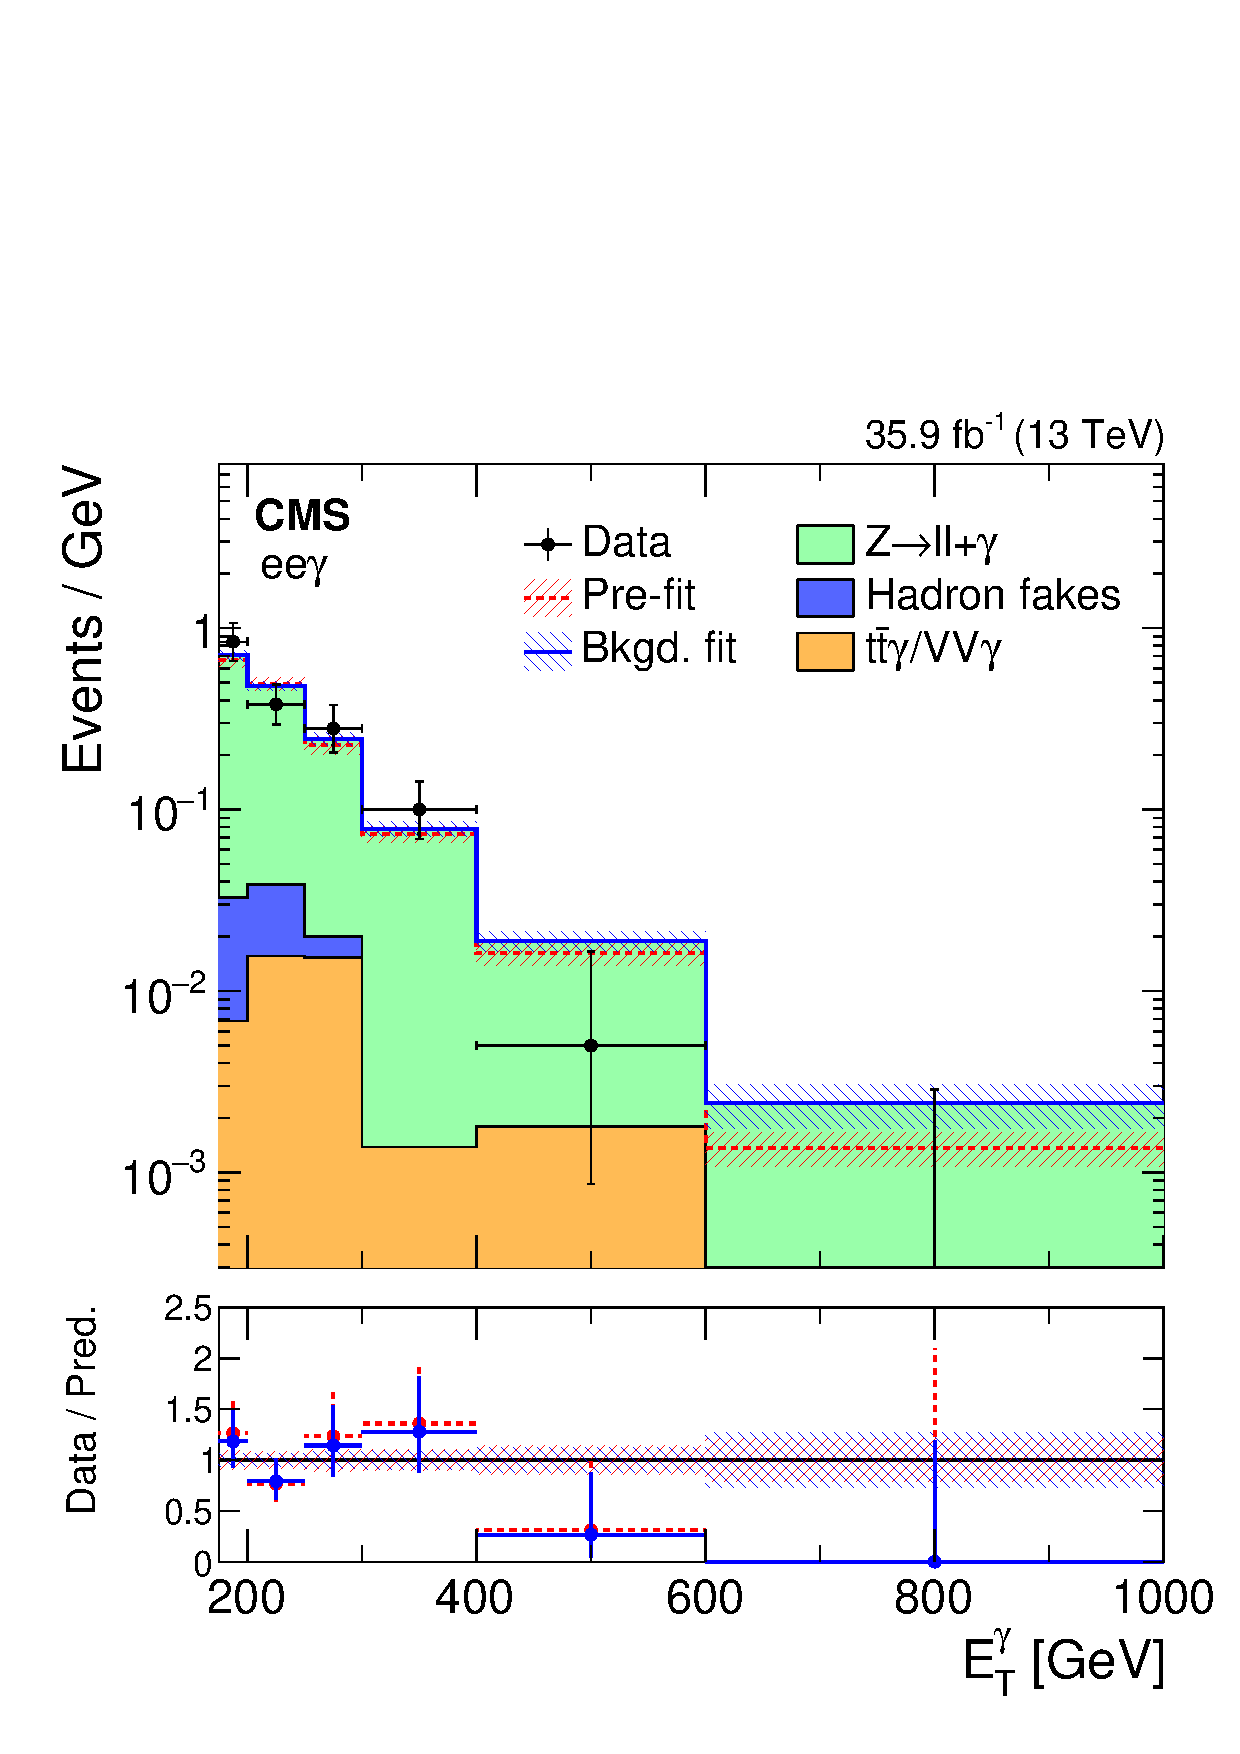
\includegraphics[width=0.45\textwidth]{Analysis/Figures/bonly_diel.pdf}
    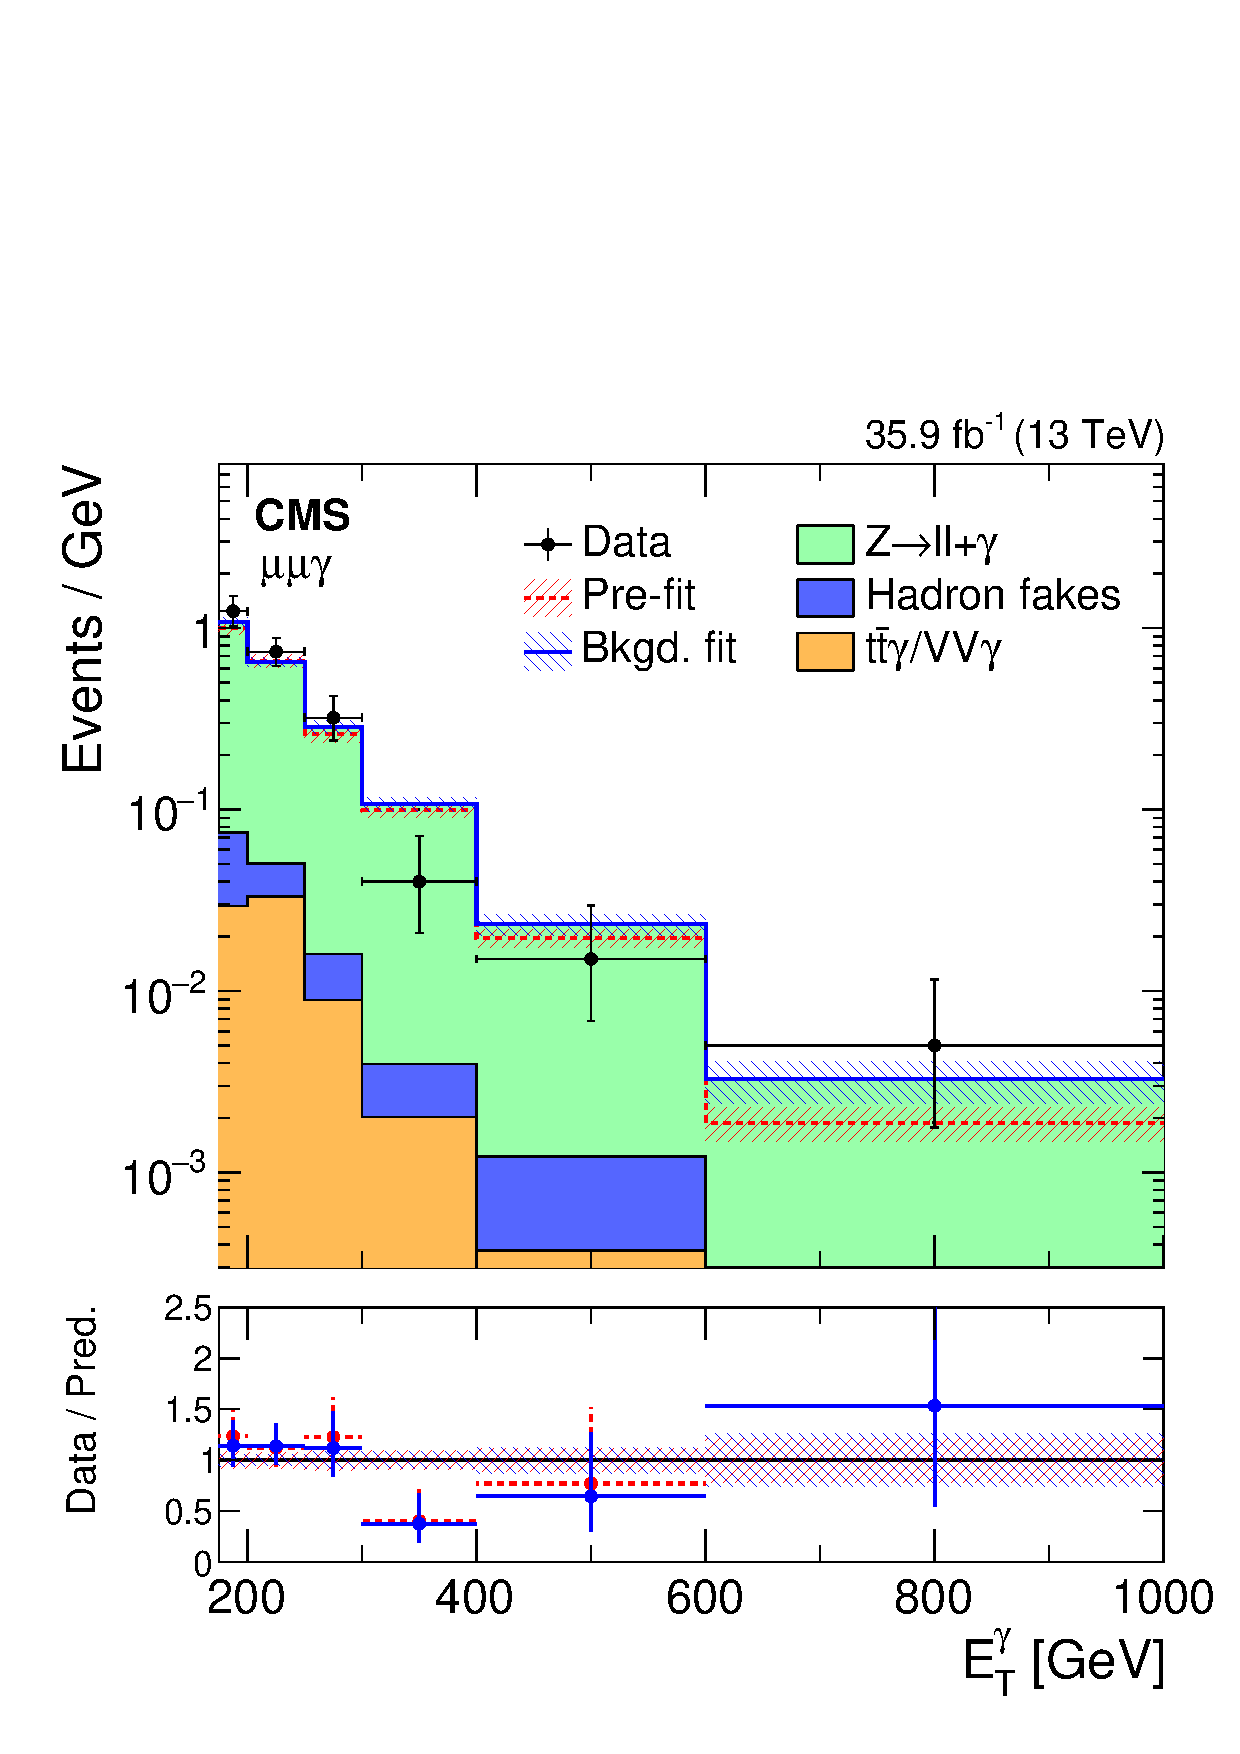
\includegraphics[width=0.45\textwidth]{Analysis/Figures/bonly_dimu.pdf}
    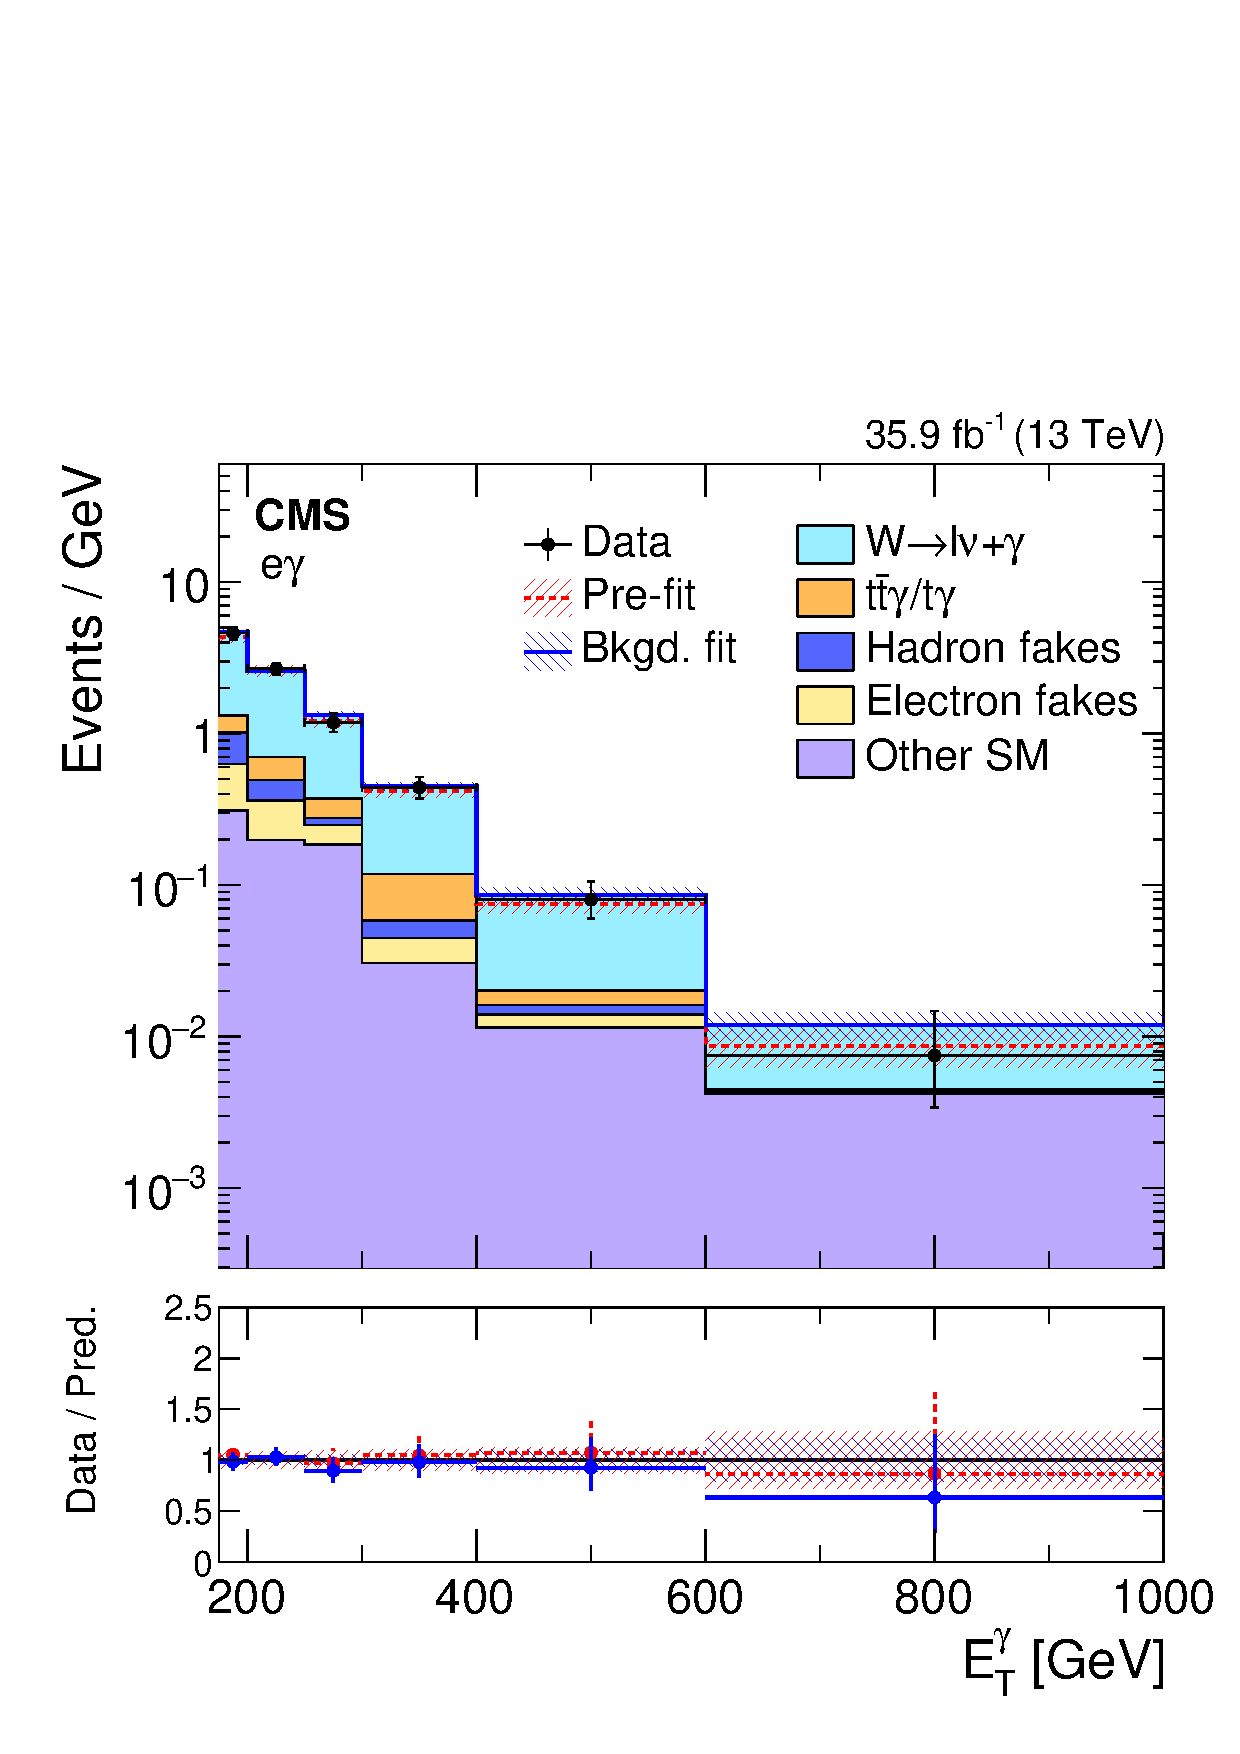
\includegraphics[width=0.45\textwidth]{Analysis/Figures/bonly_monoel.pdf}
    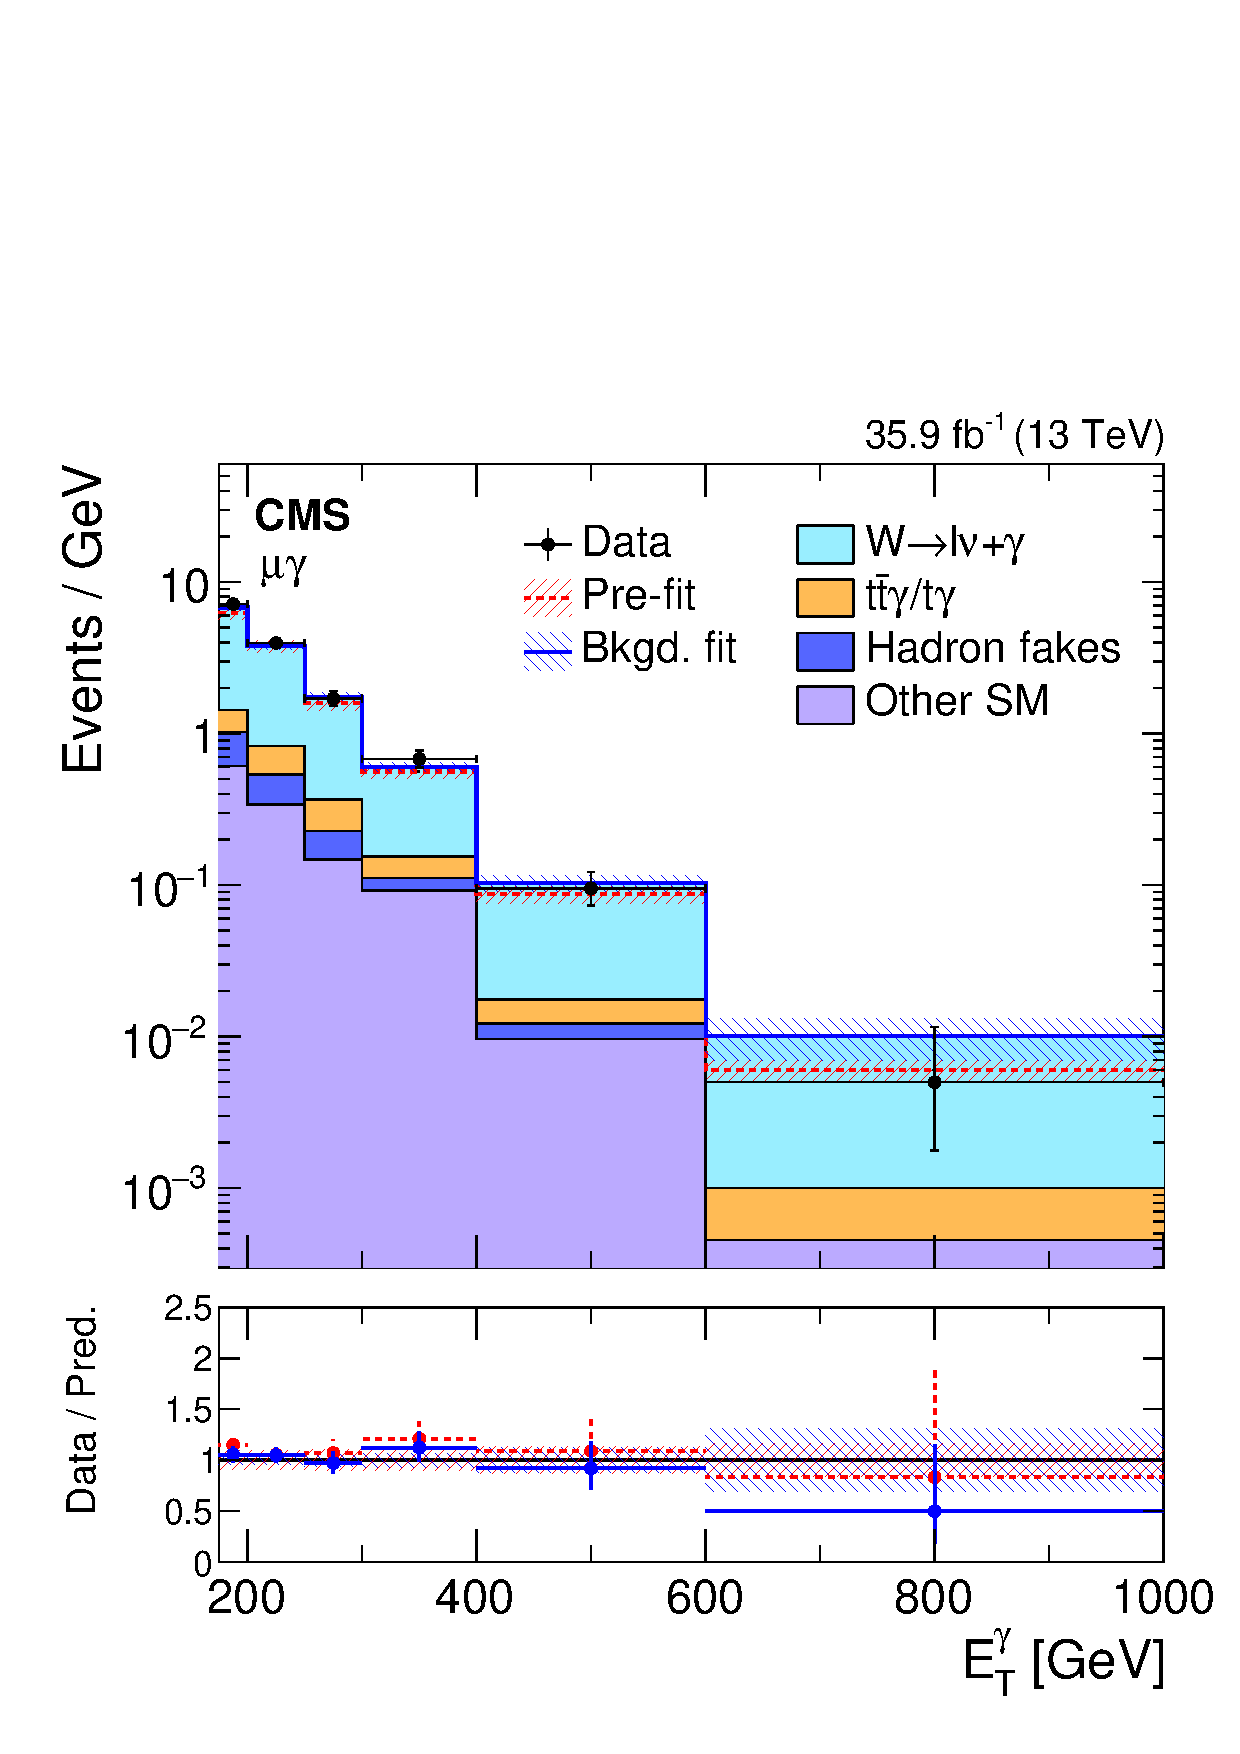
\includegraphics[width=0.45\textwidth]{Analysis/Figures/bonly_monomu.pdf}
    \caption{
      Comparison between data and MC simulation in the four control regions: 
      \Pe\Pe\Pgg\ (upper left), 
      \Pgm\Pgm\Pgg\ (upper right), 
      \Pe\Pgg\ (lower left), 
      \Pgm\Pgg\ (lower right) 
      before and after performing the simultaneous fit across all the control samples and signal region, and assuming absence of any signal.
      The last bin of the distribution includes all events with $\ETg > 1000\GeV$. 
      The ratios of data with the pre-fit background prediction (red dashed) and post-fit background prediction (blue solid) are shown in the lower panels. 
      The bands in the lower panels show the post-fit uncertainty after combining all the systematic uncertainties.
}
    \label{fig:postfitCR}
\end{figure}

\begin{figure}[htbp]
  \centering
    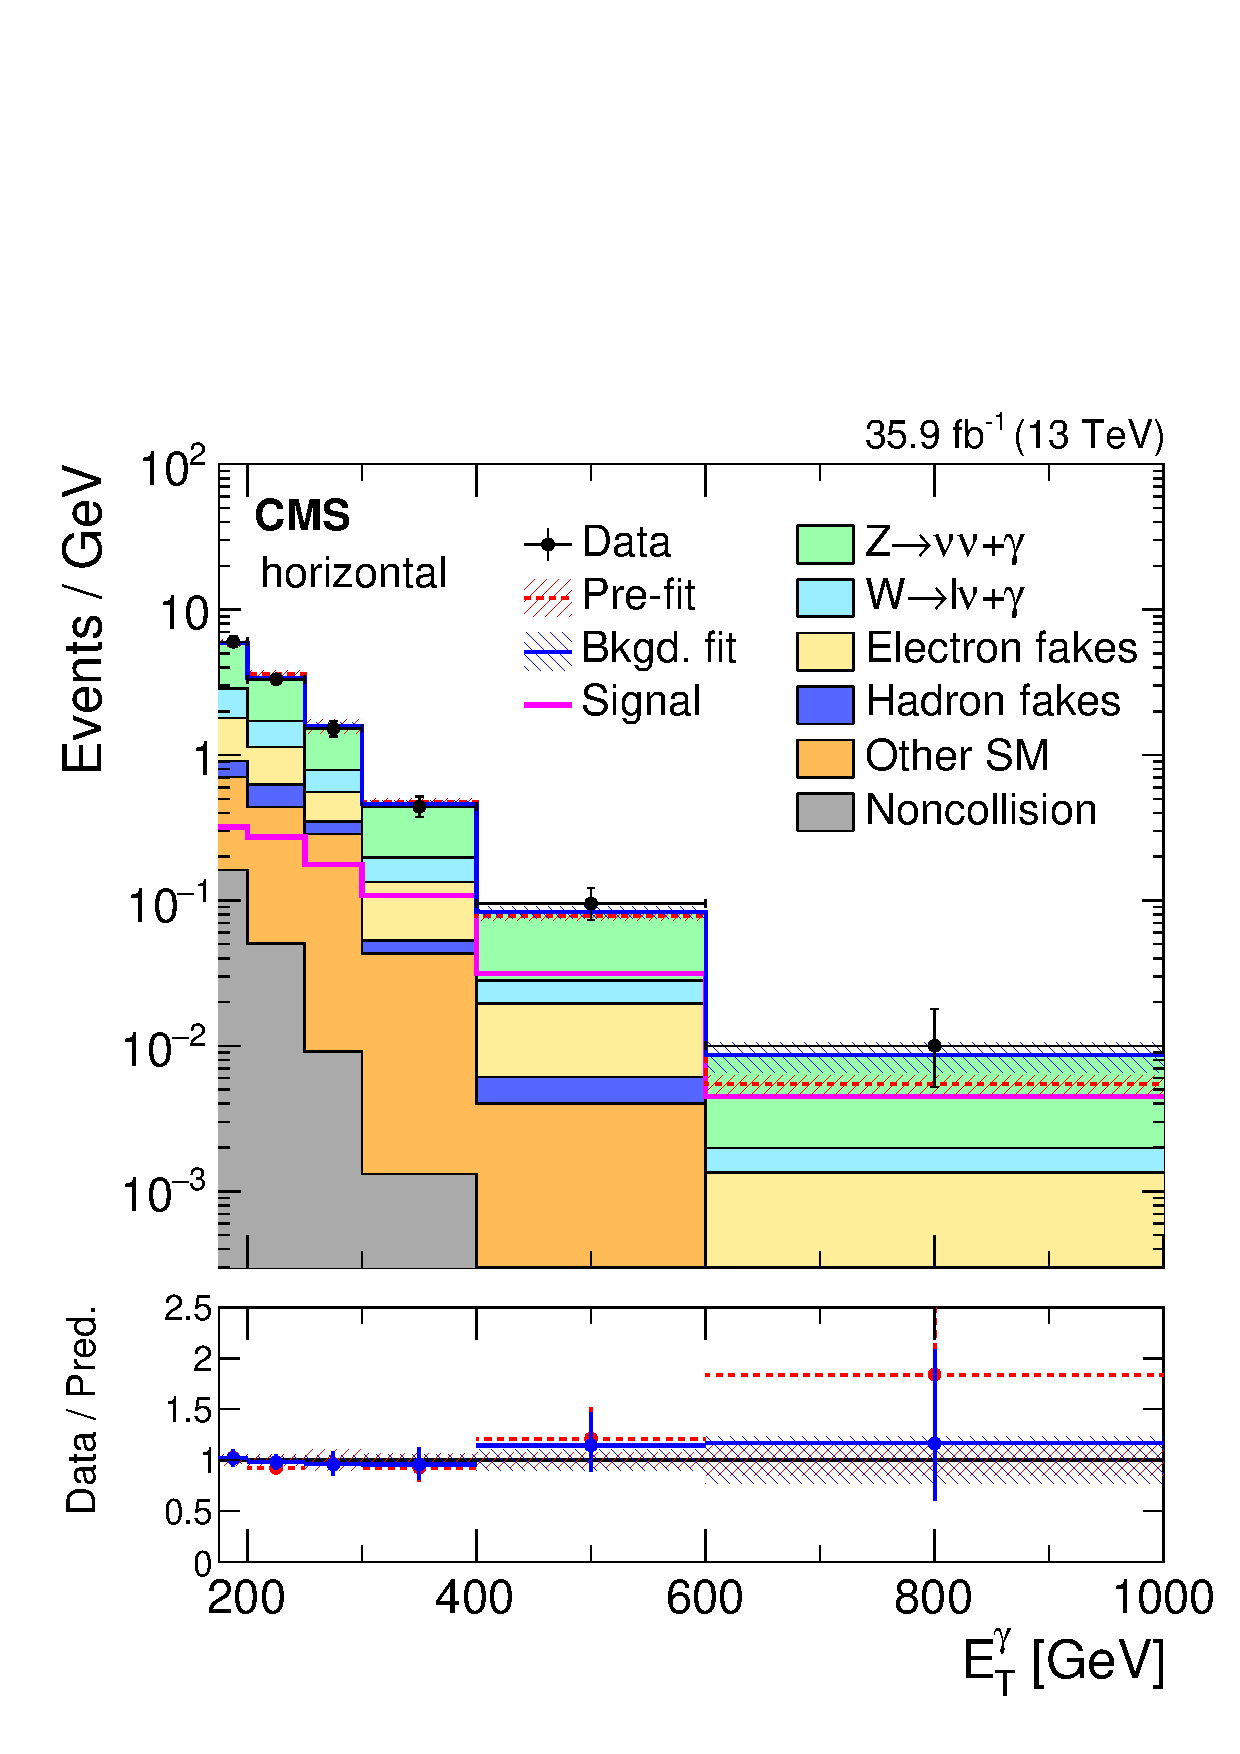
\includegraphics[width=0.45\textwidth]{Analysis/Figures/bonly_horizontal.pdf}
    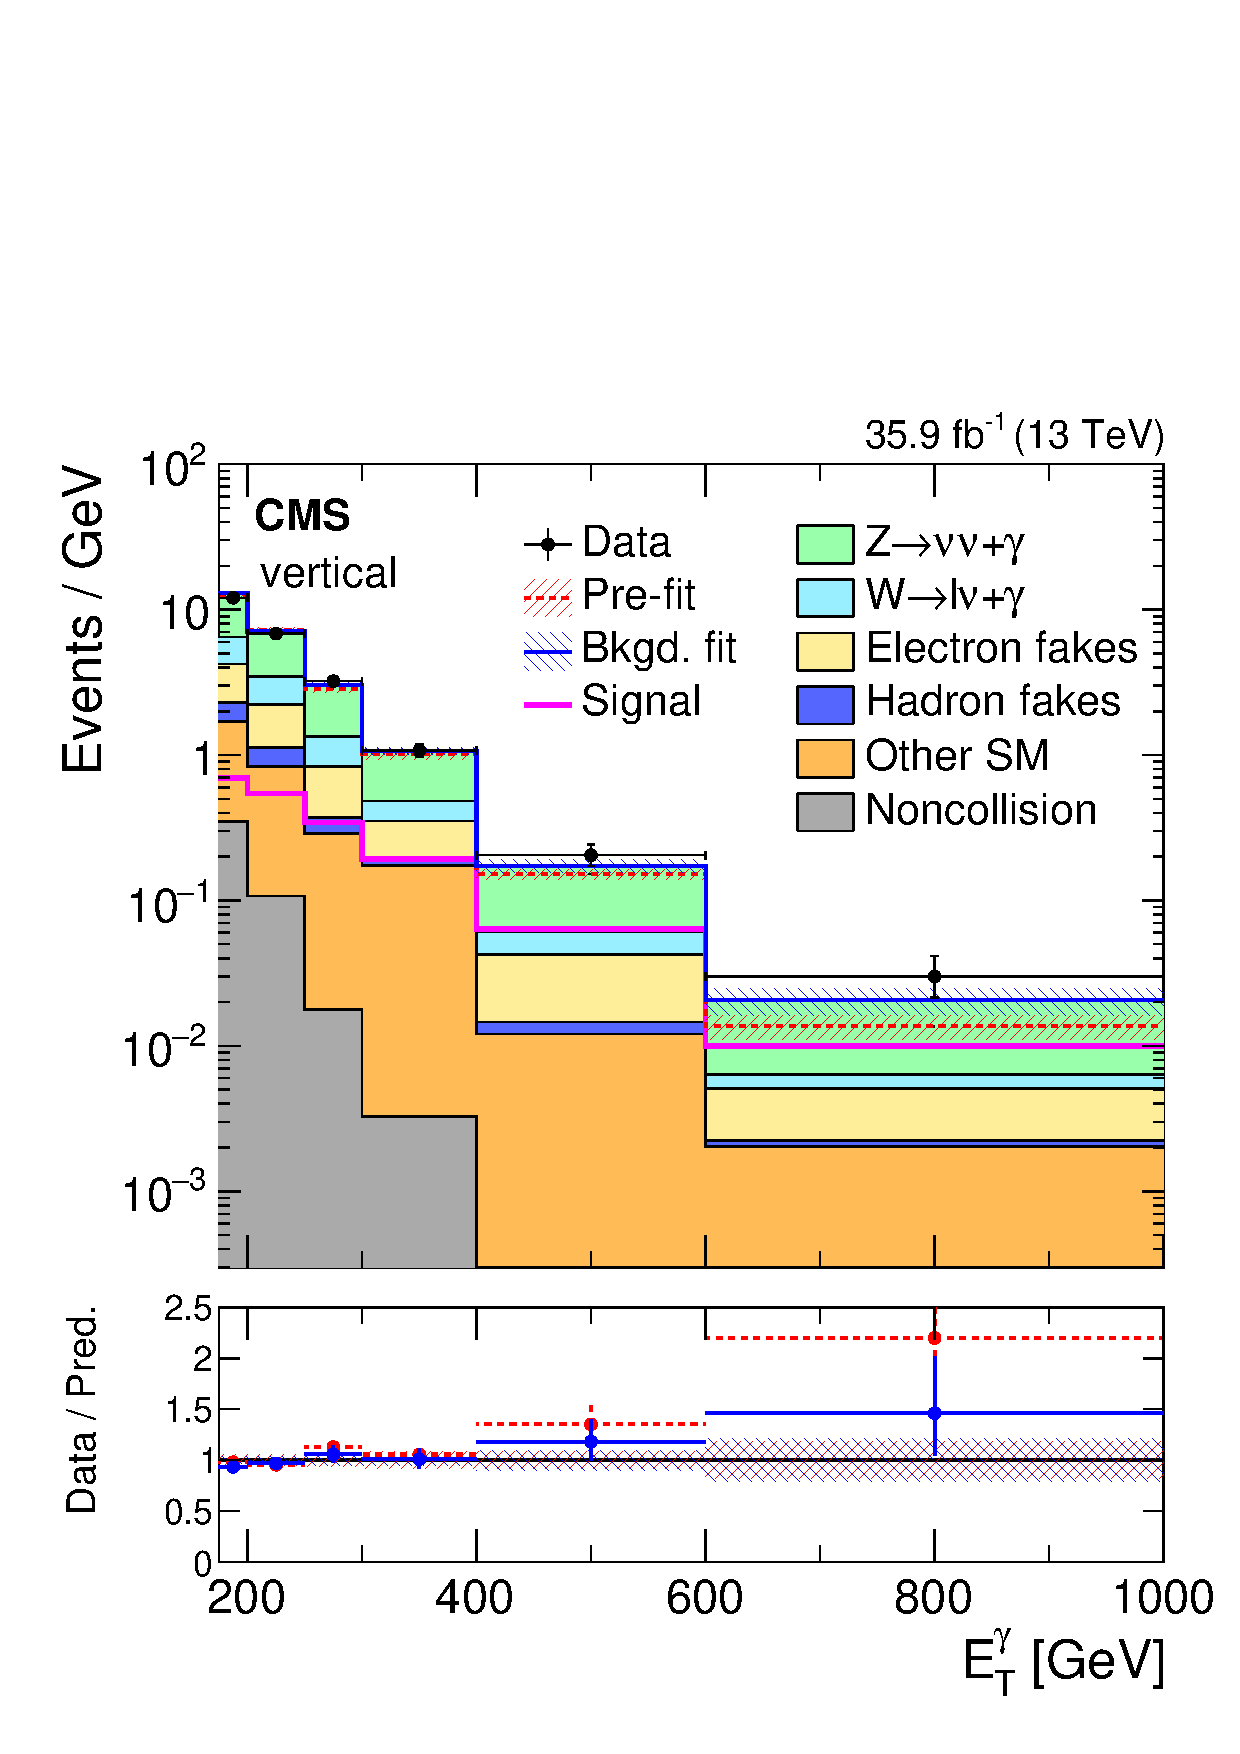
\includegraphics[width=0.45\textwidth]{Analysis/Figures/bonly_vertical.pdf}
    \caption{
      Observed \ETg\ distributions in the horizontal (left) and vertical (right) signal regions compared with the post-fit background expectations for various SM processes.
      The last bin of the distribution includes all events with $\ETg > 1000\GeV$. 
      The expected background distributions are evaluated after performing a combined fit to the data in all the control samples and the signal region. 
      The ratios of data with the pre-fit background prediction (red dashed) and post-fit background prediction (blue solid) are shown in the lower panels. 
      The bands in the lower panels show the post-fit uncertainty after combining all the systematic uncertainties. 
      The expected signal distribution from a 1\TeV vector mediator decaying to 1\GeV DM particles is overlaid.
    }
    \label{fig:postfitSR}
\end{figure}

Figure~\ref{fig:postfitCR} shows the observed \ETg\ distributionsin the four control regions compared with the results from simulations before and after performing the simultaneous fit across all the control samples and signal region, and assuming absence of any signal.
Figure~\ref{fig:postfitSR} shows the observed \ETg\ distributions in the horizontal and vertical signal regions compared with the results from simulations before and after performing a combined fit to the data in all the control samples and the signal region. 
The observed distributions are in agreement with the prediction from SM and noncollision backgrounds.

\begin{table}[htbp]
\centering
\caption{Expected event yields in each \ETg\ bin for various background processes in the horizontal signal region.
         The background yields and the corresponding uncertainties are obtained after performing a combined fit to data in all the control samples, excluding data in the signal region.
         The observed event yields in the horizontal signal region are also reported.}
\label{tab:yield_mask_horizontal}
\begin{tabular}{ lcccccc }
\hline
\rule[-1.2ex]{0pt}{3.8ex}\ETg~[\GeVns{}]      &         [175,  200] &         [200,  250] &         [250,  300] &         [300,  400] &         [400,  600] &         [600, 1000] \\
\hline
$\PZ\Pgg$        & $  81.2 \pm   8.0 $ & $  88.2 \pm   8.4 $ & $  38.8 \pm   4.8 $ & $  26.8 \pm   3.7 $ & $   8.8 \pm   1.9 $ & $   1.4 \pm   0.7 $ \\
$\PW\Pgg$        & $  27.9 \pm   3.7 $ & $  29.9 \pm   3.9 $ & $  11.4 \pm   1.7 $ & $   6.3 \pm   1.2 $ & $   1.4 \pm   0.4 $ & $   0.1 \pm   0.1 $ \\
Misid. electrons & $  22.5 \pm   2.7 $ & $  25.7 \pm   2.7 $ & $  10.5 \pm   1.0 $ & $   8.2 \pm   0.7 $ & $   2.7 \pm   0.2 $ & $   0.5 \pm   0.0 $ \\
Misid. hadrons   & $   5.2 \pm   2.2 $ & $   9.3 \pm   1.8 $ & $   3.1 \pm   0.7 $ & $   1.0 \pm   0.3 $ & $   0.4 \pm   0.1 $ & $   0.0 \pm   0.0 $ \\
Other SM         & $  13.6 \pm   2.0 $ & $  19.6 \pm   1.3 $ & $  13.9 \pm   0.4 $ & $   4.2 \pm   0.2 $ & $   0.8 \pm   0.0 $ & $   0.1 \pm   0.0 $ \\
ECAL spikes      & $   4.3 \pm   1.3 $ & $   2.7 \pm   0.8 $ & $   0.5 \pm   0.1 $ & $   0.1 \pm   0.0 $ & $   0.0 \pm   0.0 $ & $   0.0 \pm   0.0 $ \\
Total prediction & $ 154.6 \pm   8.3 $ & $ 175.4 \pm   8.8 $ & $  78.2 \pm   5.3 $ & $  46.6 \pm   4.0 $ & $  14.1 \pm   2.1 $ & $   2.1 \pm   0.8 $ \\
Observed         & $ 150   \pm  12   $ & $ 166   \pm    13 $ & $  76.0 \pm   8.7 $ & $  44.0 \pm   6.6 $ & $  19.0 \pm   4.4 $ & $   4.0 \pm   2.0 $ \\
\hline
\end{tabular}
\end{table}

\begin{table}[htbp]
\centering
\caption{Expected event yields in each \ETg\ bin for various background processes in the vertical signal region.
         The background yields and the corresponding uncertainties are obtained after performing a combined fit to data in all the control samples, excluding data in the signal regions.
         The observed event yields in the vertical signal region are also reported.}
\label{tab:yield_mask_vertical}
\begin{tabular}{ lcccccc }
\hline
\rule[-1.2ex]{0pt}{3.8ex}\ETg~[\GeVns{}]      &         [175,  200] &         [200,  250] &         [250,  300] &         [300,  400] &         [400,  600] &         [600, 1000] \\
\hline
$\PZ\Pgg$        & $ 172   \pm    17 $ & $ 190   \pm  18   $ & $  83   \pm  10   $ & $  58.6 \pm   7.9 $ & $  18.0 \pm   3.9 $ & $   3.1 \pm   1.6 $ \\
$\PW\Pgg$        & $  59.9 \pm   7.8 $ & $  63.6 \pm   7.8 $ & $  24.6 \pm   3.5 $ & $  13.4 \pm   2.4 $ & $   3.0 \pm   0.8 $ & $   0.3 \pm   0.2 $ \\
Misid. electrons & $  48.4 \pm   5.6 $ & $  56.2 \pm   5.1 $ & $  23.4 \pm   1.8 $ & $  15.7 \pm   1.4 $ & $   5.6 \pm   0.4 $ & $   1.2 \pm   0.1 $ \\
Misid. hadrons   & $  15.1 \pm   4.4 $ & $  14.5 \pm   3.1 $ & $   4.2 \pm   0.8 $ & $   2.3 \pm   0.8 $ & $   0.5 \pm   0.1 $ & $   0.1 \pm   0.1 $ \\
Other SM         & $  33.8 \pm   4.1 $ & $  36.6 \pm   2.7 $ & $  13.6 \pm   0.5 $ & $  17.1 \pm   0.6 $ & $   2.4 \pm   0.1 $ & $   0.8 \pm   0.0 $ \\
ECAL spikes      & $   9.3 \pm   2.8 $ & $   5.7 \pm   1.7 $ & $   0.9 \pm   0.3 $ & $   0.3 \pm   0.1 $ & $   0.0 \pm   0.0 $ & $   0.0 \pm   0.0 $ \\
Total prediction & $ 339   \pm  18  $ & $ 366   \pm  19   $ & $ 150   \pm  11   $ & $ 107.5 \pm   8.7 $ & $  29.6 \pm   4.3 $ & $   5.4 \pm   1.7 $ \\
Observed         & $ 301   \pm  17   $ & $ 342   \pm  19   $ & $ 161 \pm  13   $ & $ 107   \pm  10   $ & $  41.0 \pm   6.4 $ & $  12.0 \pm   3.5 $ \\
\hline
\end{tabular}
\end{table}

The expected yields in each bin of \ETg\ for all backgrounds in the horizontal and vertical signal regions after performing a combined fit to data in all the control samples, excluding data in the signal regions, are given in Tables~\ref{tab:yield_mask_horizontal} and~\ref{tab:yield_mask_vertical}, respectively.
The covariances between the predicted background yields across all the \ETg~bins in the two signal regions are shown in Fig.~\ref{fig:correlation_matrix}.
The expected yields together with the covariances can be used with the simplified likelihood
approach detailed in Ref.~\cite{CMS-NOTE-2017-001} to reinterpret the results for models not studied in this thesis

\begin{figure}[hbtp]
  \centering
  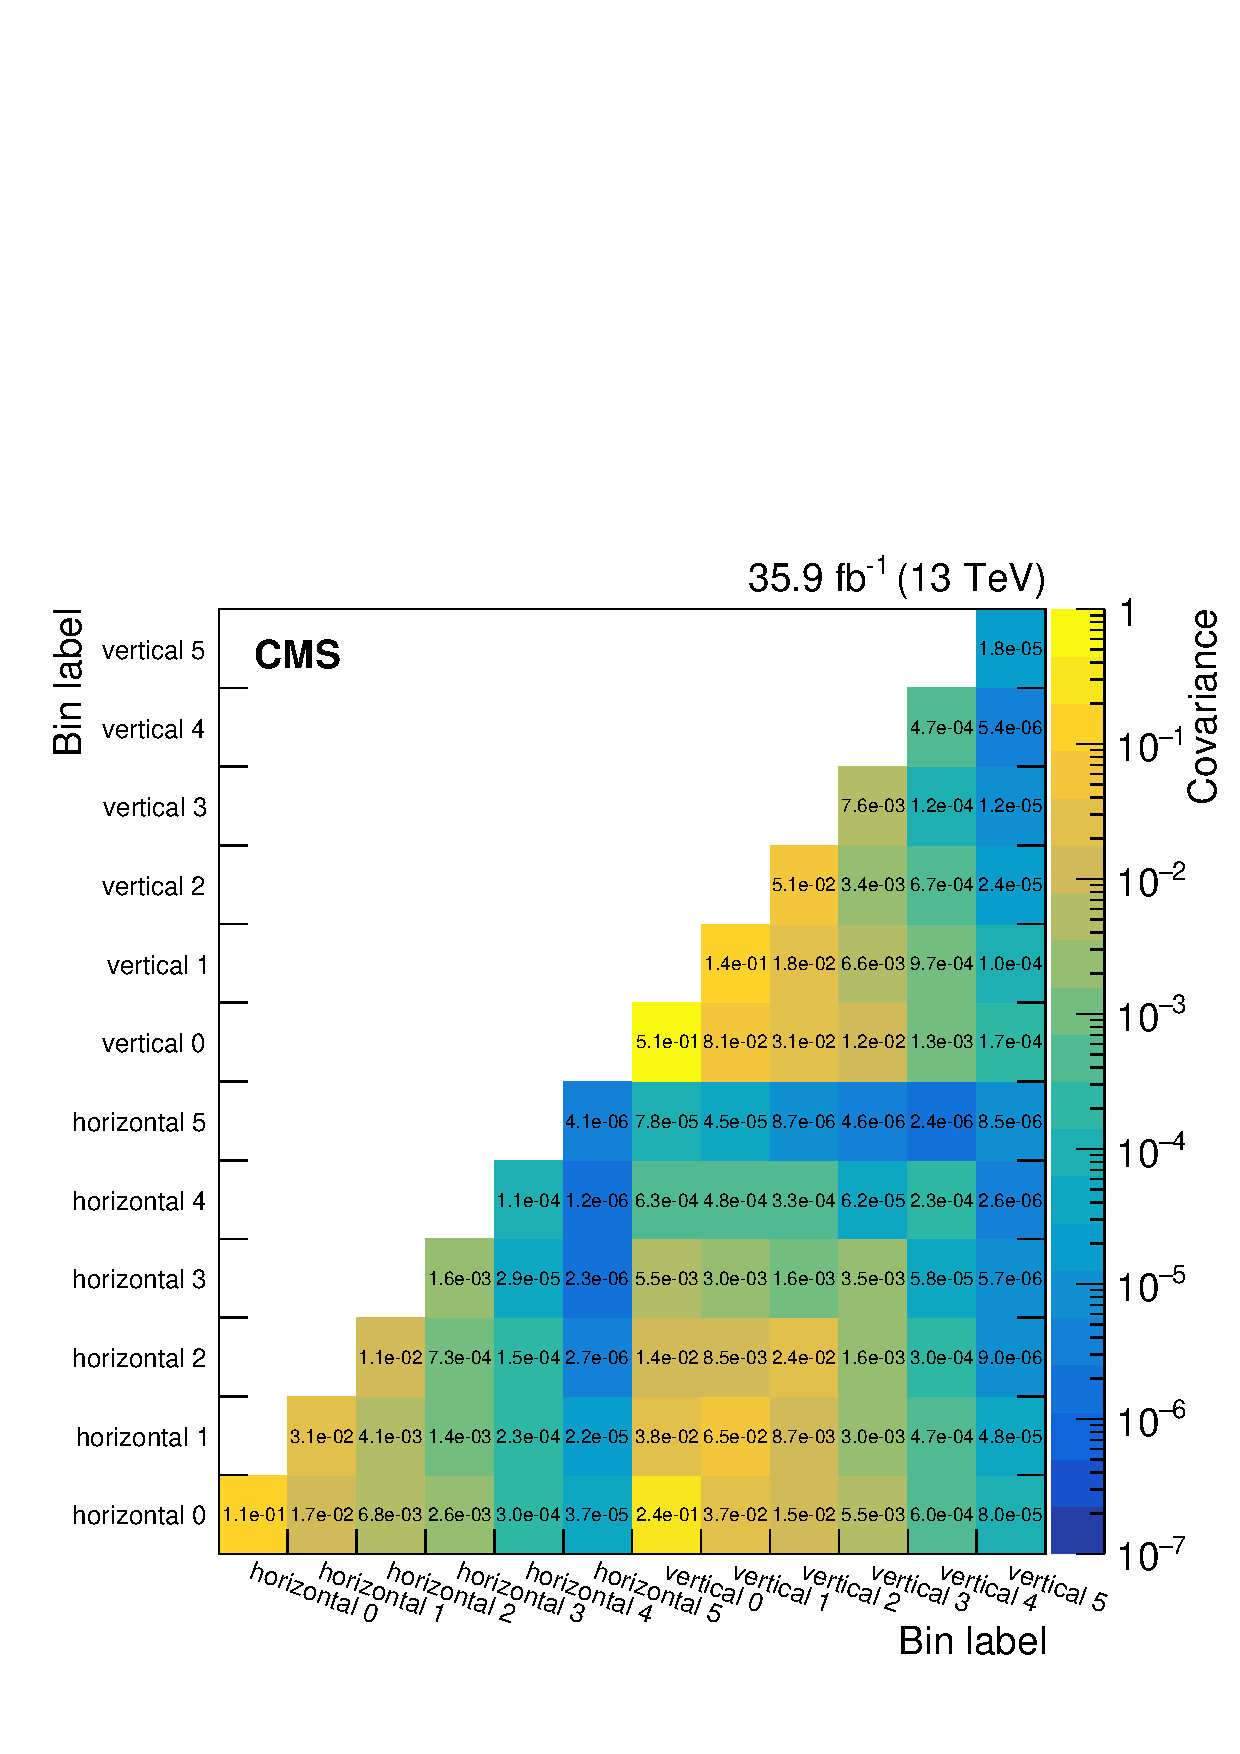
\includegraphics[width=0.9\textwidth]{Analysis/Figures/correlation_matrix.pdf}
  \caption{
    Covariances between the predicted background yields in all the \ETg\ bins of the horizontal and vertical signal regions.
    The bin labels specify which signal region the bin belongs to and what number bin it is for that region.}
  \label{fig:correlation_matrix}
\end{figure}.

\subsection{Limits}
\label{subsec:limits}

\begin{figure}[htbp]
  \centering
   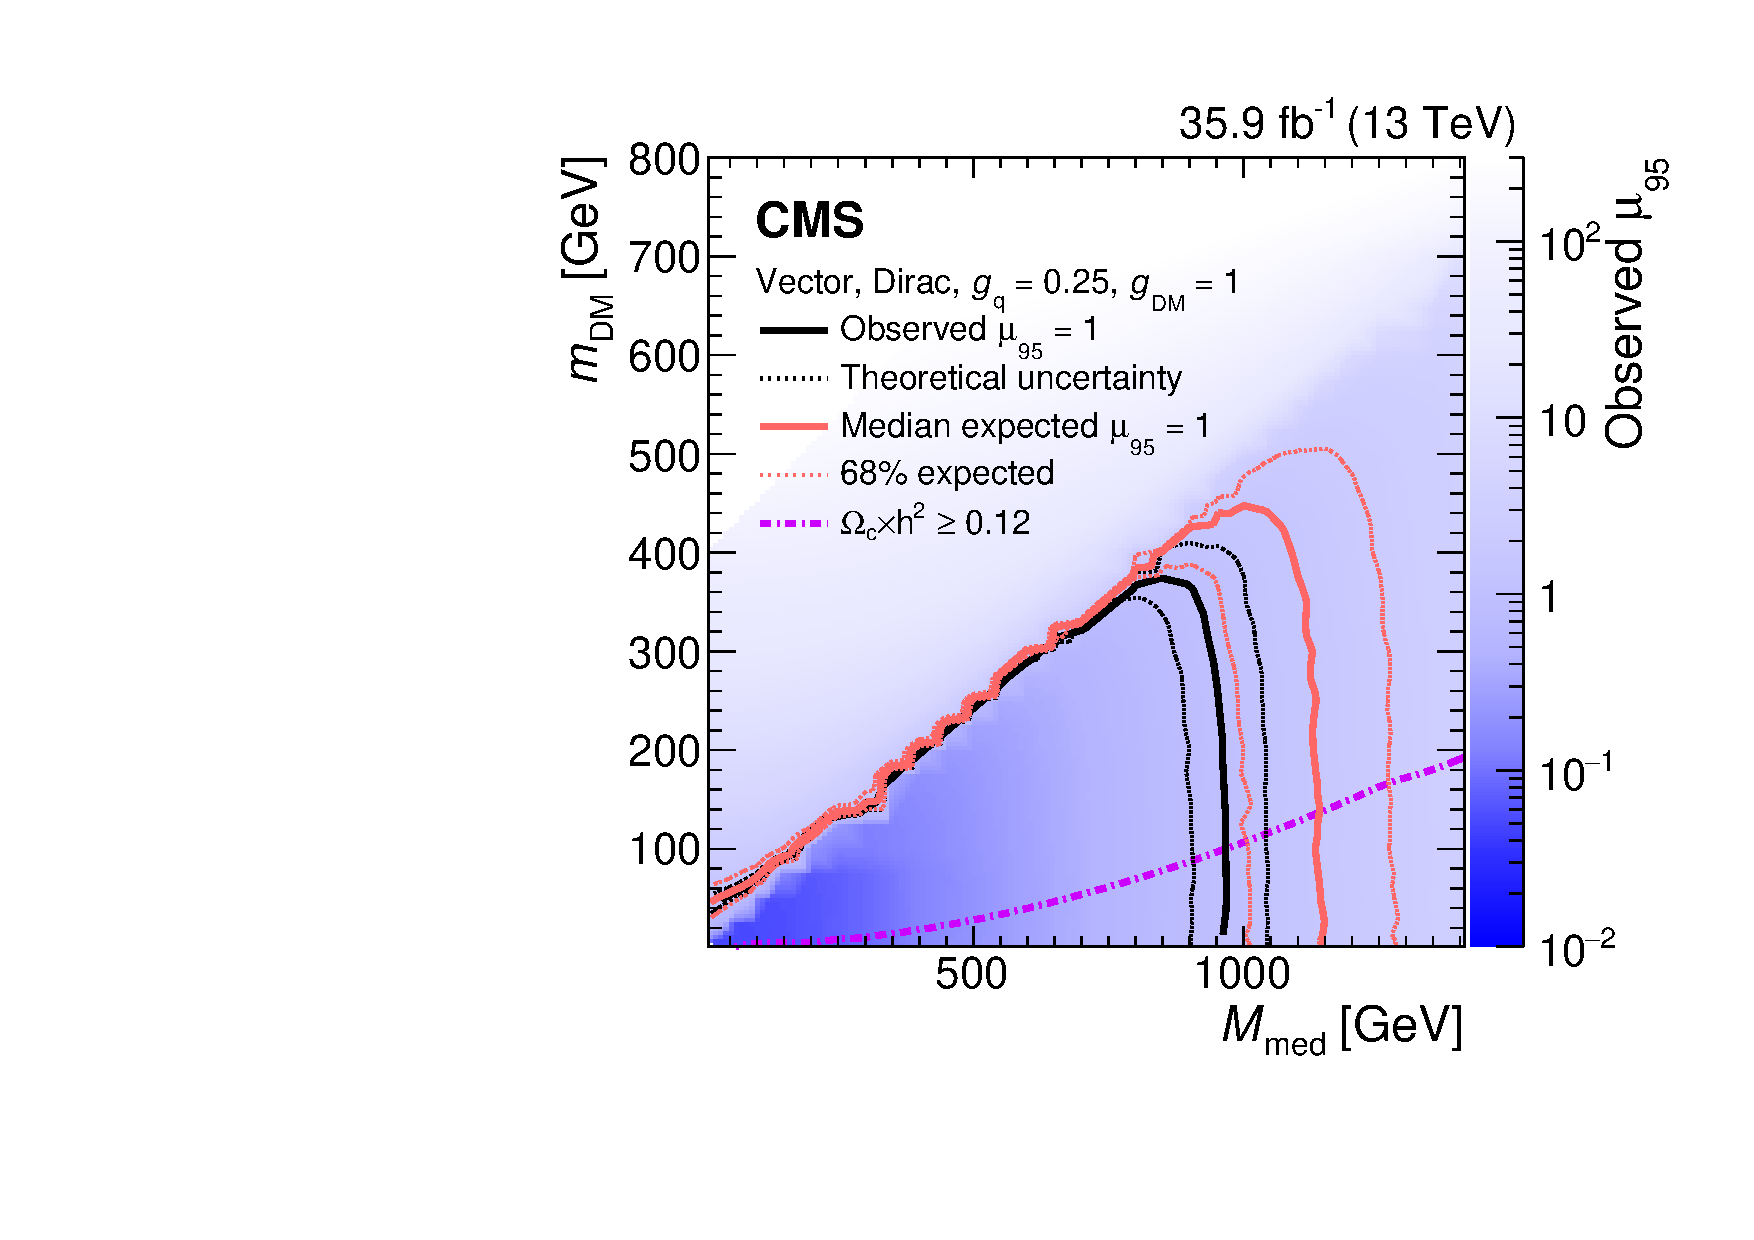
\includegraphics[width=0.48\linewidth]{Analysis/Figures/limits_vector.pdf}
    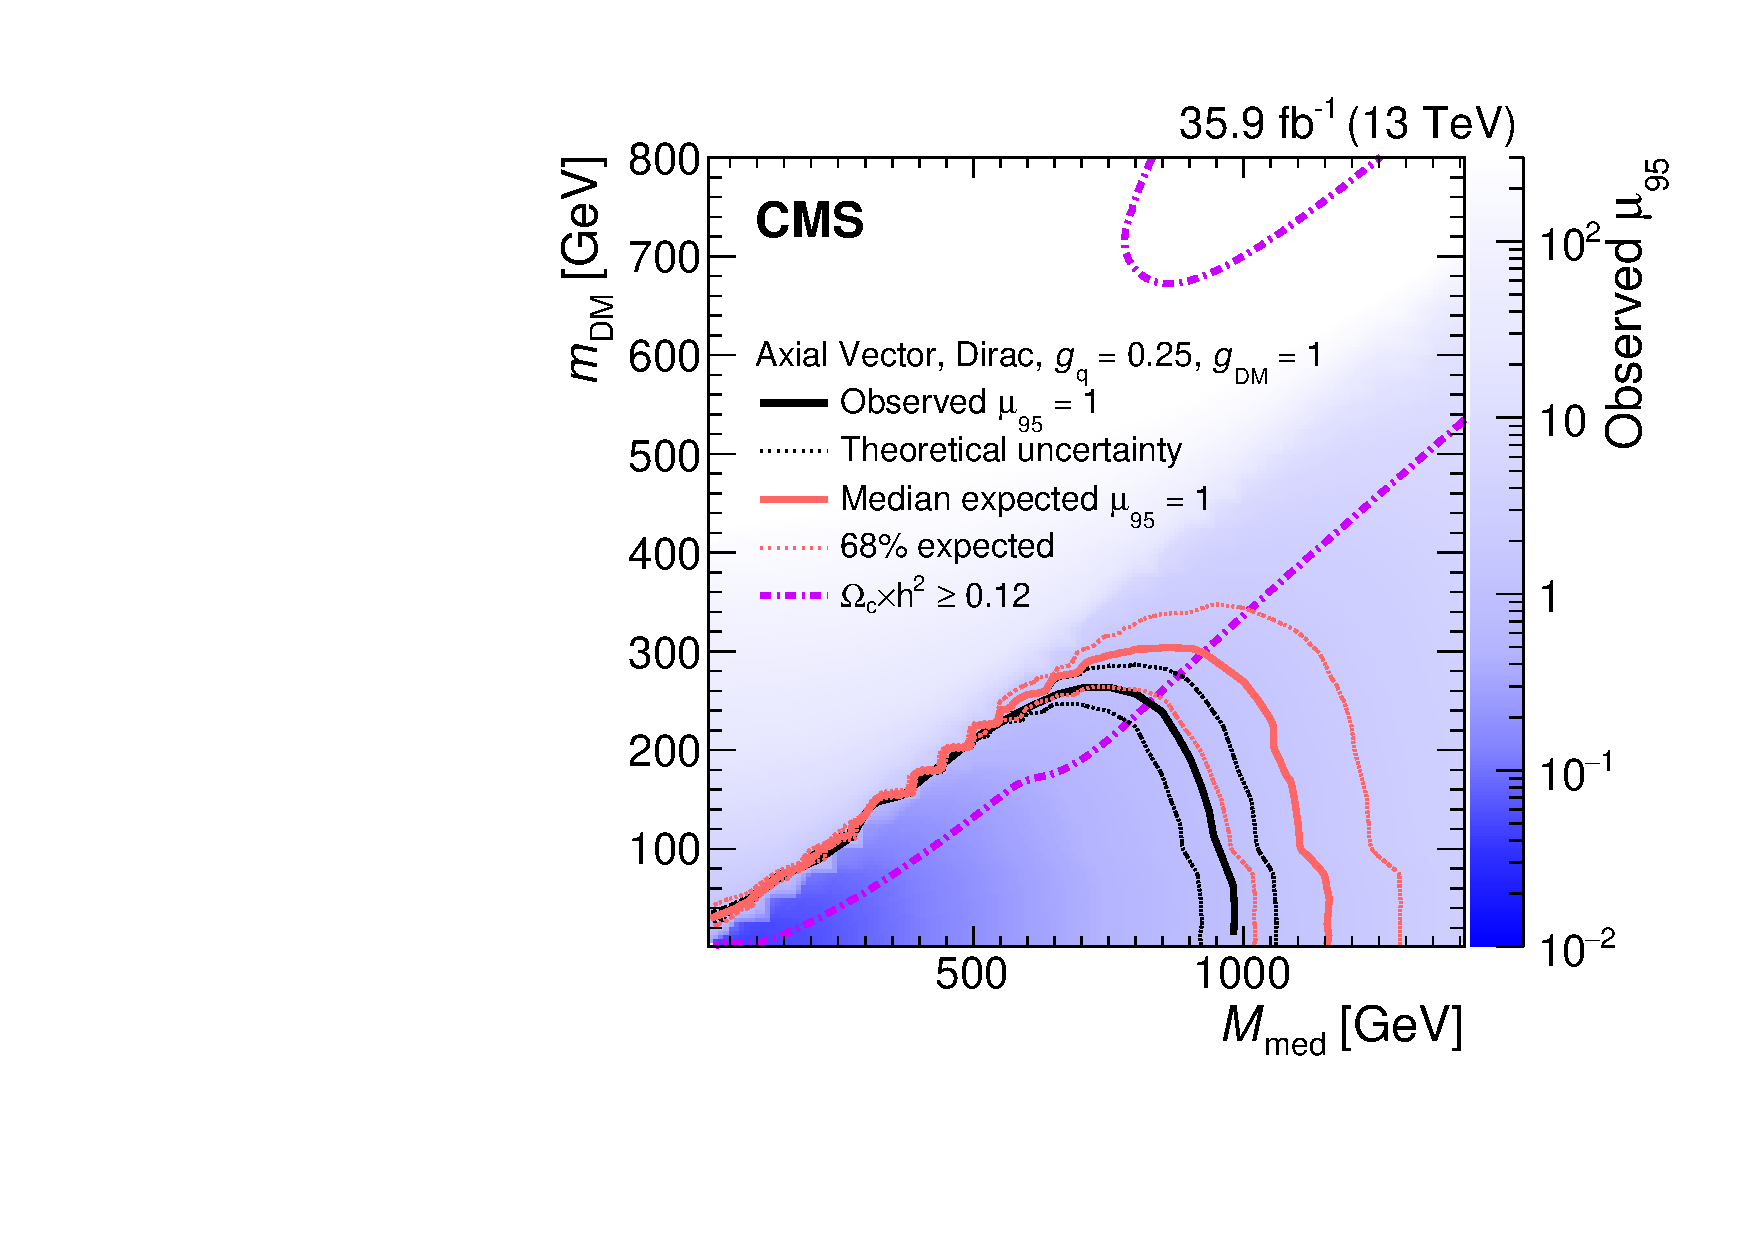
\includegraphics[width=0.48\linewidth]{Analysis/Figures/limits_axial.pdf}
    \caption{
      The ratio of 95\% \CL\ upper cross section limits to the theoretical cross section ($\mu_{95}$), for DM simplified models with vector (left) and axial-vector (right) mediators, assuming $\gq=0.25$ and $\gDM=1$.
      Expected $\mu_{95} = 1$ contours are overlaid in red. 
      The region under the observed contour is excluded. For DM simplified model parameters in the region below the lower violet dot--dash contour, and also above the corresponding upper contour in the right hand plot, cosmological DM abundance exceeds the density observed by the Planck satellite experiment.
    }
    \label{fig:limits}
\end{figure}

Figure~\ref{fig:limits} shows the 95\% \CL\ upper cross section limits with respect to the corresponding theoretical cross section ($\mu_{95}= \sigma_{95\%}/\sigma_{\text{theory}}$) for the  vector and axial-vector mediator scenarios, in the \mmed--\mdm\ plane. 
The solid black (dashed red) curves are the observed (expected) contours of $\mu_{95} = 1$. 
The $\sigma_{\text{theory}}$ hypothesis is excluded at 95\% \CL\ or above in the region with $\mu_{95} < 1$. 
The uncertainty in the expected upper limit includes the experimental uncertainties. 
For the simplified DM LO models considered, mediator masses up to 950\GeV are excluded for values of \mdm\ less than 1\GeV.
